        %%******************************************%%
        %%                                          %%
        %%        Modello di tesi di laurea         %%
        %%            di Andrea Giraldin            %%
        %%                                          %%
        %%             2 novembre 2012              %%
        %%                                          %%
        %%******************************************%%

%**************************************************************
% file contenente le impostazioni della tesi
%**************************************************************


%**************************************************************
% Impostazioni di impaginazione
% see: http://wwwcdf.pd.infn.it/AppuntiLinux/a2547.htm
%**************************************************************

% I seguenti commenti speciali impostano:
% 1. 
% 2. PDFLaTeX come motore di composizione;
% 3. tesi.tex come documento principale;
% 4. il controllo ortografico italiano per l'editor.

% !TEX encoding = UTF-8
% !TEX TS-program = pdflatex
% !TEX root = tesi.tex
% !TEX spellcheck = it-IT

% PDF/A filecontents
%\RequirePackage{filecontents}
%\begin{filecontents*}{\jobname.xmpdata}
%  \Title{Document’s title}
%  \Author{Author’s name}
%  \Language{it-IT}
%  \Subject{The abstract, or short description.}
%  \Keywords{keyword1\sep keyword2\sep keyword3}
%\end{filecontents*}

\documentclass[10pt,                    % corpo del font principale
               a4paper,                 % carta A4
               oneside,                 % impagina per fronte-retro 
               openright,               % inizio capitoli a destra
               english,                 
               italian,                 
               ]{book}    

%**************************************************************
% Importazione package
%************************************************************** 

\PassOptionsToPackage{dvipsnames}{xcolor} % colori PDF/A

\usepackage{colorprofiles}

\usepackage[a-2b,mathxmp]{pdfx}[2018/12/22]
                                        % configurazione PDF/A
                                        % validare in https://www.pdf-online.com/osa/validate.aspx

%\usepackage{amsmath,amssymb,amsthm}    % matematica

\usepackage[T1]{fontenc}                
\usepackage{lmodern}                    % codifica dei font:
                                        % NOTA BENE! richiede una distribuzione *completa* di LaTeX

\usepackage[utf8]{inputenc}             % codifica di input; anche [latin1] va bene
                                        % NOTA BENE! va accordata con le preferenze dell'editor

\usepackage[english, italian]{babel}    % per scrivere in italiano e in inglese;
                                        % l'ultima lingua (l'italiano) risulta predefinita

\usepackage{bookmark}                   % segnalibri

\usepackage{caption}                    % didascalie

\usepackage{chngpage,calc}              % centra il frontespizio

\usepackage{csquotes}                   % gestisce automaticamente i caratteri (")

\usepackage{emptypage}                  % pagine vuote senza testatina e piede di pagina

\usepackage{epigraph}			% per epigrafi

\usepackage{eurosym}                    % simbolo dell'euro

%\usepackage{indentfirst}               % rientra il primo paragrafo di ogni sezione

\usepackage{graphicx}                   % immagini

\usepackage{hyperref}                   % collegamenti ipertestuali

\usepackage[binding=5mm]{layaureo}      % margini ottimizzati per l'A4; rilegatura di 5 mm

\usepackage{listings}                   % codici

\usepackage{microtype}                  % microtipografia

%\usepackage{mparhack,fixltx2e,relsize}  % finezze tipografiche

\usepackage{nameref}                    % visualizza nome dei riferimenti                                      
\usepackage[font=small]{quoting}        % citazioni

\usepackage{subfig}                     % sottofigure, sottotabelle

\usepackage[italian]{varioref}          % riferimenti completi della pagina

\usepackage{booktabs}                   % tabelle                                       
\usepackage{tabularx}                   % tabelle di larghezza prefissata                                    
\usepackage{longtable}                  % tabelle su più pagine                                        
\usepackage{ltxtable}                   % tabelle su più pagine e adattabili in larghezza
\usepackage{xcolor}                     % colore tabelle
\usepackage{color, colortbl}

\usepackage[toc, acronym]{glossaries}   % glossario
                                        % per includerlo nel documento bisogna:
                                        % 1. compilare una prima volta tesi.tex;
                                        % 2. eseguire: makeindex -s tesi.ist -t tesi.glg -o tesi.gls tesi.glo
                                        % 3. eseguire: makeindex -s tesi.ist -t tesi.alg -o tesi.acr tesi.acn
                                        % 4. compilare due volte tesi.tex.

\usepackage[backend=biber,style=verbose-ibid,hyperref,backref]{biblatex}
                                        % eccellente pacchetto per la bibliografia; 
                                        % produce uno stile di citazione autore-anno; 
                                        % lo stile "numeric-comp" produce riferimenti numerici
                                        % per includerlo nel documento bisogna:
                                        % 1. compilare una prima volta tesi.tex;
                                        % 2. eseguire: biber tesi
                                        % 3. compilare ancora tesi.tex.
                                        
\usepackage{float}                      % for float option[H]

%**************************************************************
% Header con logo 
%**************************************************************
\usepackage{fancyhdr}                   %for fancy fancy
\newcolumntype{L}[1]{>{\raggedright\let\newline\\\arraybackslash}m{#1}}
\newcolumntype{C}[1]{>{\centering\let\newline\\\arraybackslash}m{#1}}
\newcolumntype{R}[1]{>{\raggedleft\let\newline\\\arraybackslash}m{#1}}
\newcommand{\aCapo}{ ~ \vspace{0.25cm} \\} %magari fare renewcommand di paragraph 

\pagestyle{fancy}
\fancyhead[R]{Tesi di Laurea}
\fancyhead[L]{
    
\includegraphics[width=0.8cm]{immagini/ds_logo.png}
}
\fancyfoot[C]{\thepage}

\fancypagestyle{plain}{
    \fancyhead[R]{Tesi di Laurea}
    \fancyhead[L]{
        
\includegraphics[width=0.8cm]{immagini/ds_logo.png}
    }
    \fancyfoot[C]{\thepage}
}

%riduzione spacing tra header e "Capitolo XX"
\usepackage{titlesec}
\titleformat{\chapter}[display]   
{\normalfont\huge\bfseries}{\chaptertitlename\ \thechapter}{20pt}{\Huge}   
\titlespacing*{\chapter}{0pt}{-18pt}{40pt}

%**************************************************************

%\usepackage{minted} %For code in appendix

%**************************************************************
% Frontespizio
%**************************************************************

% Autore
\newcommand{\myName}{Giacomo Sassaro}                                    
\newcommand{\myTitle}{Sviluppo di un'app multipiattaforma legata al mondo wellness con Flutter}

% Tipo di tesi                   
\newcommand{\myDegree}{Tesi di laurea}

% Università             
\newcommand{\myUni}{Università degli Studi di Padova}

% Facoltà       
\newcommand{\myFaculty}{Corso di Laurea Triennale in Informatica}

% Dipartimento
\newcommand{\myDepartment}{Dipartimento di Matematica "Tullio Levi-Civita"}

% Titolo del relatore
\newcommand{\profTitle}{Prof. }

% Relatore
\newcommand{\myProf}{Paolo Baldan}

% Luogo
\newcommand{\myLocation}{Padova}

% Anno accademico
\newcommand{\myAA}{2020-2021}

% Data discussione
\newcommand{\myTime}{Settembre 2021}


                   % file con le impostazioni personali


\setlength{\parindent}{14pt}   % larghezza rientro della prima riga
\setlength{\parskip}{0pt}   % distanza tra i paragrafi



%**************************************************************
% Impostazioni di biblatex
%**************************************************************
\bibliography{bibliografia} % database di biblatex 

\defbibheading{bibliography} {
    \cleardoublepage
    \phantomsection 
    \addcontentsline{toc}{chapter}{\bibname}
    \chapter*{\bibname\markboth{\bibname}{\bibname}}
}

\setlength\bibitemsep{1.5\itemsep} % spazio tra entry

\DeclareBibliographyCategory{opere}
\DeclareBibliographyCategory{web}

\addtocategory{opere}{womak:lean-thinking}
\addtocategory{web}{site:agile-manifesto}

\defbibheading{opere}{\section*{Riferimenti bibliografici}}
\defbibheading{web}{\section*{Siti Web consultati}}


%**************************************************************
% Impostazioni di caption
%**************************************************************
\captionsetup{
    tableposition=top,
    figureposition=bottom,
    font=small,
    format=hang,
    labelfont=bf
}

%**************************************************************
% Impostazioni di glossaries
%**************************************************************

%**************************************************************
% Acronimi
%**************************************************************
\renewcommand{\acronymname}{Acronimi e abbreviazioni}

\newacronym[description={\glslink{apig}{Application Program Interface}}]
    {api}{API}{Application Program Interface}

\newacronym[description={\glslink{umlg}{Unified Modeling Language}}]
    {uml}{UML}{Unified Modeling Language}

\newacronym[description={\glslink{mvpg}{Model View Presenter}}]
    {mvp}{MVP}{Model View Presenter}

%**************************************************************
% Glossario
%**************************************************************
%\renewcommand{\glossaryname}{Glossario}
\renewcommand{\glsnamefont}[1]{\makefirstuc{#1}}


\newglossaryentry{branch}
{
    name=branch,
    sort=branch,
    description={Rappresenta una linea di sviluppo indipendente e serve come astrazione per il processo di modifica,
stage o commit.}
}
\newglossaryentry{fork}
{
    name=fork,
    sort=fork,
    description={Sviluppo di un nuovo progetto software che parte dal codice sorgente di un altro già esistente}
}

\newglossaryentry{pull request}
{
    name=pull request,
    sort=pull request,
    description={È una richiesta, fatta all’autore originale di un sofware o di un documento, di includere le nostre personali modifiche al suo progetto. Una pull request controlla automaticamente se sono presenti conflitti tra i file da unire.}
}

\newglossaryentry{agile}
{
    name=agile,
    sort=agile,
    description={È un modello di sviluppo che si contrappone ai classici modelli a cascata o incrementali proponendo un approccio meno strutturato e focalizzato sull'obiettivo di consegnare al cliente, in tempi brevi e frequentemente, software funzionante e di qualità. }
}
\newglossaryentry{BMI}
{
    name=BMI,
    sort=bmi,
    description={Body Mass Index è un dato biometrico, espresso come rapporto tra peso e quadrato dell'altezza di un individuo ed è utilizzato come un indicatore dello stato di peso forma. }
}
\newglossaryentry{bot}
{
    name=bot,
    sort=bot,
    description={Con la parola “bot”, abbreviazione di “robot”, in informatica si intende un programma che ha accesso agli stessi sistemi di comunicazione e interazione con le macchine usate dagli esseri umani.}
}

\newglossaryentry{JWT}
{
    name=JWT,
    sort=jwt,
    description={JSON Web Token è uno standard Internet proposto per la creazione di dati con firma opzionale e/o crittografia opzionale il cui payload contiene un JSON che afferma un certo numero di attestazioni. I token vengono firmati utilizzando una crittografica simmetrica o asimmetrica utilizzando una coppia di chaivi pubblica/privata.}
}
\newglossaryentry{gamification}
{
    name=gamification,
    sort=gamification,
    description={È l'utilizzo di elementi mutuati dai giochi e delle tecniche di game design in contesti non ludici. L'idea è quella di coinvolgere le persone a provare più divertimento e partecipazione nelle attività quotidiane ricche di azioni monotone e noiose attraverso il gioco.}
}
\newglossaryentry{SDK}
{
    name=SDK,
    sort=sdk,
    description={Un Software Developer Kit è un insieme di strumenti per lo sviluppo e la documentazione di software}
}

\newglossaryentry{SRP}
{
    name=SRP,
    sort=srp,
    description={Il Single Responsability Princile afferma che ogni elemento di un programma deve avere una sola responsabilità, e che tale responsabilità debba essere interamente incapsulata dall'elemento stesso. Tutti i servizi offerti dall'elemento dovrebbero essere strettamente allineati a tale responsabilità. }
}
\newglossaryentry{codebase}
{
    name=codebase,
    sort=codebase,
    description={Collezione di codice sorgente usata per costruire una particolare applicazione o un particolare componente.}
}
 % database di termini
\makeglossaries


%**************************************************************
% Impostazioni di graphicx
%**************************************************************
\graphicspath{{immagini/}} % cartella dove sono riposte le immagini


%**************************************************************
% Impostazioni di hyperref
%**************************************************************
\hypersetup{
    %hyperfootnotes=false,
    %pdfpagelabels,
    %draft,	% = elimina tutti i link (utile per stampe in bianco e nero)
    colorlinks=true,
    linktocpage=true,
    pdfstartpage=1,
    pdfstartview=,
    % decommenta la riga seguente per avere link in nero (per esempio per la stampa in bianco e nero)
    %colorlinks=false, linktocpage=false, pdfborder={0 0 0}, pdfstartpage=1, pdfstartview=FitV,
    breaklinks=true,
    pdfpagemode=UseNone,
    pageanchor=true,
    pdfpagemode=UseOutlines,
    plainpages=false,
    bookmarksnumbered,
    bookmarksopen=true,
    bookmarksopenlevel=1,
    hypertexnames=true,
    pdfhighlight=/O,
    %nesting=true,
    %frenchlinks,
    urlcolor=webbrown,
    linkcolor=RoyalBlue,
    citecolor=webgreen,
    %pagecolor=RoyalBlue,
    %urlcolor=Black, linkcolor=Black, citecolor=Black, %pagecolor=Black,
    %pdftitle={\myTitle},
    %pdfauthor={\textcopyright\ \myName, \myUni, \myFaculty},
    %pdfsubject={},
    %pdfkeywords={},
    %pdfcreator={pdfLaTeX},
    %pdfproducer={LaTeX}
}

%**************************************************************
% Impostazioni di itemize
%**************************************************************
\renewcommand{\labelitemi}{$\bullet$}

%\renewcommand{\labelitemi}{$\bullet$}
%\renewcommand{\labelitemii}{$\cdot$}
%\renewcommand{\labelitemiii}{$\diamond$}
%\renewcommand{\labelitemiv}{$\ast$}


%**************************************************************
% Impostazioni di listings
%**************************************************************
\lstset{
    language=[LaTeX]Tex,%C++,
    keywordstyle=\color{RoyalBlue}, %\bfseries,
    basicstyle=\small\ttfamily,
    %identifierstyle=\color{NavyBlue},
    commentstyle=\color{Green}\ttfamily,
    stringstyle=\rmfamily,
    numbers=none, %left,%
    numberstyle=\scriptsize, %\tiny
    stepnumber=5,
    numbersep=8pt,
    showstringspaces=false,
    breaklines=true,
    frameround=ftff,
    frame=single
} 
\colorlet{punct}{red!60!black}
\definecolor{background}{HTML}{EEEEEE}
\definecolor{delim}{RGB}{20,105,176}
\colorlet{numb}{magenta!60!black}
\definecolor{codegreen}{rgb}{0,0.6,0}
\definecolor{codegray}{rgb}{0.5,0.5,0.5}
\definecolor{codepurple}{rgb}{0.82, 0.62, 0.91}
\definecolor{codeblue}{rgb}{0, 0.5, 1}
\definecolor{codeorange}{rgb}{1, 0.22, 0}

% Define the codebox
\lstdefinelanguage{dart}{
backgroundcolor=\color{background},   
    commentstyle=\color{codegreen},
    basicstyle=\ttfamily\footnotesize,
    breakatwhitespace=false,         
    breaklines=true, 
    stepnumber=1,
    captionpos=b,                    
    keepspaces=true,                 
    numbers=left,                    
    numbersep=8pt,                  
    showspaces=false,                
    showstringspaces=false,
    showtabs=false,                  
    tabsize=2,
    %frame=shadowbox
    emph=[1]{CheckLogin, HookWidget, Widget, BuildContext, bool, String, int, List, GenericErrorPage, LoginScreen, LoadUser, LoadCoach, DelayedWidget, Widget, Key, this, super, Future, false, true, Duration, Waiter, List, Goals, Appointment, ChangeNotifierProvider, UserRepo, Provider, ChangeNotifier, Reader, User, Options, Dio, Future },% Insert here the types you are using
    emphstyle=[1]{\color{codeblue}},
    emph=[2]{useProvider, build, useState, useEffect, delayed, then, buildCards, addAll, buildGoalsCards, where, map, toList, buildAppointmentCards, getAccessToken, fetchUser, watch, notifyListeners},% Insert here the methods you are using
    emphstyle=[2]{\color{codepurple}},
    emph=[3]{class, extends, @override, if, return, else, switch, case, default, final, required, is, as, =>, async, void, try, catch, finally, await},% Insert here the keywords you are using
    emphstyle=[3]{\color{codeorange}},%
}

\lstdefinelanguage{json}{
    basicstyle=\ttfamily\footnotesize,
    numbers=left,
    numberstyle=\scriptsize,
    stepnumber=1,
    numbersep=8pt,
    showstringspaces=false,
    breaklines=true,
    backgroundcolor=\color{background},
    string=[s]{"}{"},
    stringstyle=\color{blue},
    comment=[l]{:},
    commentstyle=\color{black},
    literate=
     *{0}{{{\color{numb}0}}}{1}
      {1}{{{\color{numb}1}}}{1}
      {2}{{{\color{numb}2}}}{1}
      {3}{{{\color{numb}3}}}{1}
      {4}{{{\color{numb}4}}}{1}
      {5}{{{\color{numb}5}}}{1}
      {6}{{{\color{numb}6}}}{1}
      {7}{{{\color{numb}7}}}{1}
      {8}{{{\color{numb}8}}}{1}
      {9}{{{\color{numb}9}}}{1}
      {:}{{{\color{punct}{:}}}}{1}
      {,}{{{\color{punct}{,}}}}{1}
      {[}{{{\color{delim}{[}}}}{1}
      {]}{{{\color{delim}{]}}}}{1},
}


%**************************************************************
% Impostazioni di xcolor
%**************************************************************
\definecolor{webgreen}{rgb}{0,.5,0}
\definecolor{webbrown}{rgb}{.6,0,0}


%**************************************************************
% Altro
%**************************************************************

\newcommand{\omissis}{[\dots\negthinspace]} % produce [...]

% eccezioni all'algoritmo di sillabazione
\hyphenation
{
    ma-cro-istru-zio-ne
    gi-ral-din
}

\newcommand{\sectionname}{sezione}
\addto\captionsitalian{\renewcommand{\figurename}{Figura}
                       \renewcommand{\tablename}{Tabella}}

\newcommand{\glsfirstoccur}{\ap{{[g]}}}

\newcommand{\intro}[1]{\emph{\textsf{#1}}}

%**************************************************************
% Environment per ``rischi''
%**************************************************************
\newcounter{riskcounter}                % define a counter
\setcounter{riskcounter}{0}             % set the counter to some initial value

%%%% Parameters
% #1: Title
\newenvironment{risk}[1]{
    \refstepcounter{riskcounter}        % increment counter
    \par \noindent                      % start new paragraph
    \textbf{\arabic{riskcounter}. #1}   % display the title before the 
                                        % content of the environment is displayed 
}{
    \par\medskip
}

\newcommand{\riskname}{Rischio}

\newcommand{\riskdescription}[1]{\textbf{\\Descrizione:} #1.}

\newcommand{\risksolution}[1]{\textbf{\\Soluzione:} #1.}

%**************************************************************
% Environment per ``use case''
%**************************************************************
\newcounter{usecasecounter}             % define a counter
\setcounter{usecasecounter}{0}          % set the counter to some initial value

%%%% Parameters
% #1: ID
% #2: Nome
\newenvironment{usecase}[2]{
    \renewcommand{\theusecasecounter}{\usecasename #1}  % this is where the display of 
                                                        % the counter is overwritten/modified
    \refstepcounter{usecasecounter}             % increment counter
    \vspace{10pt}
    \par \noindent                              % start new paragraph
    {\large \textbf{\usecasename #1: #2}}       % display the title before the 
                                                % content of the environment is displayed 
    \medskip
}{
    \medskip
}

\newcommand{\usecasename}{UC}

\newcommand{\usecaseactors}[1]{\textbf{\\Attori Principali:} #1. \vspace{4pt}}
\newcommand{\usecasepre}[1]{\textbf{\\Precondizioni:} #1. \vspace{4pt}}
\newcommand{\usecasedesc}[1]{\textbf{\\Descrizione:} #1. \vspace{4pt}}
\newcommand{\usecasepost}[1]{\textbf{\\Postcondizioni:} #1. \vspace{4pt}}
\newcommand{\usecasealt}[1]{\textbf{\\Scenario Alternativo:} #1. \vspace{4pt}}

%**************************************************************
% Environment per ``namespace description''
%**************************************************************

\newenvironment{namespacedesc}{
    \vspace{10pt}
    \par \noindent                              % start new paragraph
    \begin{description} 
}{
    \end{description}
    \medskip
}

\newcommand{\classdesc}[2]{\item[\textbf{#1:}] #2}
%**************************************************************
%cose mie
\definecolor{red}{cmyk}{0,0.87,0.68,0.32}
%\newcolumntype{C}[1]{>{\centering\let\newline\\\arraybackslash\hspace{0pt}}m{#1}}

\newcommand{\vsc}{\textit{Visual Studio Code}}
\newcommand{\astudio}{\textit{Android Studio}}
\newcommand{\flutter}{\textit{Flutter}}
\newcommand{\swift}{\textit{Swift}}
\newcommand{\kotlin}{\textit{Kotlin}}
\newcommand{\java}{\textit{Java}}
\newcommand{\unity}{\textit{Unity}}
\newcommand{\dart}{\textit{Dart}}
\newcommand{\arplug}{\textit{ar\_flutter\_plugin}}
\newcommand{\arcore}{\textit{ARCore}}



\begin{document}
%\pagecolor{blond} %per occhi
%**************************************************************
% Materiale iniziale
%**************************************************************
\frontmatter
% !TEX encoding = UTF-8
% !TEX TS-program = pdflatex
% !TEX root = ../tesi.tex

%**************************************************************
% Frontespizio 
%**************************************************************
\begin{titlepage}

\begin{center}

\begin{LARGE}
\textbf{\myUni}\\
\end{LARGE}

\vspace{10pt}

\begin{Large}
\textsc{\myDepartment}\\
\end{Large}

\vspace{10pt}

\begin{large}
\textsc{\myFaculty}\\
\end{large}

\vspace{30pt}
\begin{figure}[htbp]
\begin{center}

\includegraphics[height=6cm]{logo-unipd}
\end{center}
\end{figure}
\vspace{30pt} 

\begin{LARGE}
\begin{center}
\textbf{\myTitle}\\
\end{center}
\end{LARGE}

\vspace{10pt} 

\begin{large}
\textsl{\myDegree}\\
\end{large}

\vspace{40pt} 

\begin{minipage}{.48\linewidth}
\begin{flushleft}
\textit{Relatore}\\ 
\vspace{5pt} 
\profTitle \myProf
\end{flushleft}
\end{minipage}
\begin{minipage}{.48\linewidth}
\begin{flushright}
\textit{Laureando}\\ 
\vspace{5pt} 
\myName
\end{flushright}
\end{minipage}

\vspace{40pt}

\line(1, 0){338} \\
\begin{normalsize}
\textsc{Anno Accademico \myAA}
\end{normalsize}

\end{center}
\end{titlepage} 

% !TEX encoding = UTF-8
% !TEX TS-program = pdflatex
% !TEX root = ../tesi.tex

%**************************************************************
% Colophon
%**************************************************************
\clearpage
\phantomsection
\thispagestyle{empty}

\hfill

\vfill

\noindent\myName: \textit{\myTitle,}
\myDegree,
\textcopyright\ \myTime.
%% !TEX encoding = UTF-8
% !TEX TS-program = pdflatex
% !TEX root = ../tesi.tex

%**************************************************************
% Dedica
%**************************************************************
\cleardoublepage
\phantomsection
\thispagestyle{empty}
\pdfbookmark{Dedica}{Dedica}

\vspace*{3cm}

\begin{center}
Lorem ipsum dolor sit amet, consectetuer adipiscing elit. \\ \medskip
--- Oscar Wilde    
\end{center}

\medskip

\begin{center}
Dedicato a ...
\end{center}

% !TEX encoding = UTF-8
% !TEX TS-program = pdflatex
% !TEX root = ../tesi.tex

%**************************************************************
% Sommario
%**************************************************************
\cleardoublepage
\phantomsection
\pdfbookmark{Sommario}{Sommario}
\begingroup
\let\clearpage\relax
\let\cleardoublepage\relax
\let\cleardoublepage\relax

\chapter*{Sommario}

Il presente documento è il resoconto della mia attività di tirocinio, della durata di circa trecentoventi ore, presso l'azienda Datasoil S.r.l.\\
L'obiettivo principale è stato la progettazione e l'implementazione di un'applicazione multipiattaforma legata al mondo del wellness/fitness a supporto della piattaforma di analisi dati realizzata per un prodotto spinoff dell'azienda. Il tutto con un focus sull'usabilità e l'engagement/gamification.\\
Il prodotto è stato sviluppato utilizzando Dart come linguaggio di programmazione e Flutter come framework. In questo modo è stato possibile scrivere un'unica applicazione che possa funzionare sia su dispositivi Android, sia su dispositivi iOS.

%\vfill
%
%\selectlanguage{english}
%\pdfbookmark{Abstract}{Abstract}
%\chapter*{Abstract}
%
%\selectlanguage{italian}

\endgroup			

\vfill


% !TEX encoding = UTF-8
% !TEX TS-program = pdflatex
% !TEX root = ../tesi.tex

%**************************************************************
% Ringraziamenti
%**************************************************************
\cleardoublepage
\phantomsection
\pdfbookmark{Ringraziamenti}{ringraziamenti}

\bigskip

\begingroup
\let\clearpage\relax
\let\cleardoublepage\relax
\let\cleardoublepage\relax

\chapter*{Ringraziamenti}

\noindent \textit{Innanzitutto, vorrei esprimere la mia gratitudine al Prof. Paolo Baldan, relatore della mia tesi, per l'aiuto che mi ha fornito nella stesura di questo documento.}\\

\noindent \textit{Un ringraziamento speciale va ad Andrea e Pietro, che sono sempre stati disponibili quando avevo bisogno di chiarimenti, e in generale a tutto il team Datasoil S.r.l. che mi ha permesso di vivere questa esperienza in un ambiente sereno e amichevole.}\\

\noindent \textit{Desidero ringraziare con affetto la mia famiglia per il sostegno, il grande aiuto e per essermi stati vicini in ogni momento durante gli anni di studio.}\\

\noindent \textit{Infine, desidero i miei amici per tutti i bellissimi anni passati insieme e le mille avventure vissute.}\\
\bigskip

\noindent\textit{\myLocation, \myTime}
\hfill \myName

\endgroup


% !TEX encoding = UTF-8
% !TEX TS-program = pdflatex
% !TEX root = ../tesi.tex

%**************************************************************
% Indici
%**************************************************************
\cleardoublepage
\pdfbookmark{\contentsname}{tableofcontents}
\setcounter{tocdepth}{2}
\tableofcontents
%\markboth{\contentsname}{\contentsname} 
\clearpage

\begingroup 
    \let\clearpage\relax
    \let\cleardoublepage\relax
    \let\cleardoublepage\relax
    %*******************************************************
    % Elenco delle figure
    %*******************************************************    
    \phantomsection
    \pdfbookmark{\listfigurename}{lof}
    \listoffigures

    \vspace*{8ex}

    %*******************************************************
    % Elenco delle tabelle
    %*******************************************************
    \phantomsection
    \pdfbookmark{\listtablename}{lot}
    \listoftables
        
    \vspace*{8ex}
    %*******************************************************
    % Elenco dei frammenti di codice
    %*******************************************************
    \renewcommand{\lstlistingname}{Codice}
    \renewcommand{\lstlistlistingname}{Elenco dei frammenti di codice}
    \phantomsection
    \pdfbookmark{\lstlistlistingname}{lol}
    \lstlistoflistings
        
    \vspace*{8ex}
\endgroup

\cleardoublepage

\cleardoublepage

%**************************************************************
% Materiale principale
%**************************************************************
\mainmatter
% !TEX encoding = UTF-8
% !TEX TS-program = pdflatex
% !TEX root = ../tesi.tex

%**************************************************************
\chapter{Contesto Aziendale}
\label{cap:contesto-aziendale}
%**************************************************************

\section{L'azienda}
\subsection{Descrizione}
Le informazioni a seguito sono state prese direttamente dall'azienda, tuttavia ritengono siano rappresentative della realtà considerando sia il progetto al quale ho partecipato, sia il resto dell'offerta \textit{software}.\\
\textbf{Datasoil S.r.l.} è una \textit{startup} che si occupa di sviluppare applicativi dedicati alla gestione aziendale, altamente integrati con industria 4.0 e \textit{digital twin} (controparte digitale di un oggetto reale, ad esempio un macchinario di una linea produttiva): vengono impiegati apprendimento automatico\footnote{Anche detto \textit{machine learning} in inglese è una branca dell'intelligenza artificiale che utilizza metodi statistici per migliorare la performance di un algoritmo nell'identificare pattern nei dati, nella quale in una macchina si predispone l'abilità di apprendere in maniera autonoma. {\tiny Fonte: \href{https://it.wikipedia.org/wiki/Apprendimento_automatico}{Wikipedia}}} e analisi predittive per ottenere analitiche migliori rispetto alla concorrenza, con un occhio attento a innovazione, sicurezza e scalabilità, ottenute anche delegando la gestione delle componenti \textit{server} a servizi terzi come \aws{}\footnote{Ecosistema \textit{software} fornito da Amazon, che va da semplici piattaforme di \textit{cloud storage} fino a sistemi predittivi basati su \textit{machine learning}}.
\begin{figure}[H]
    \centering
    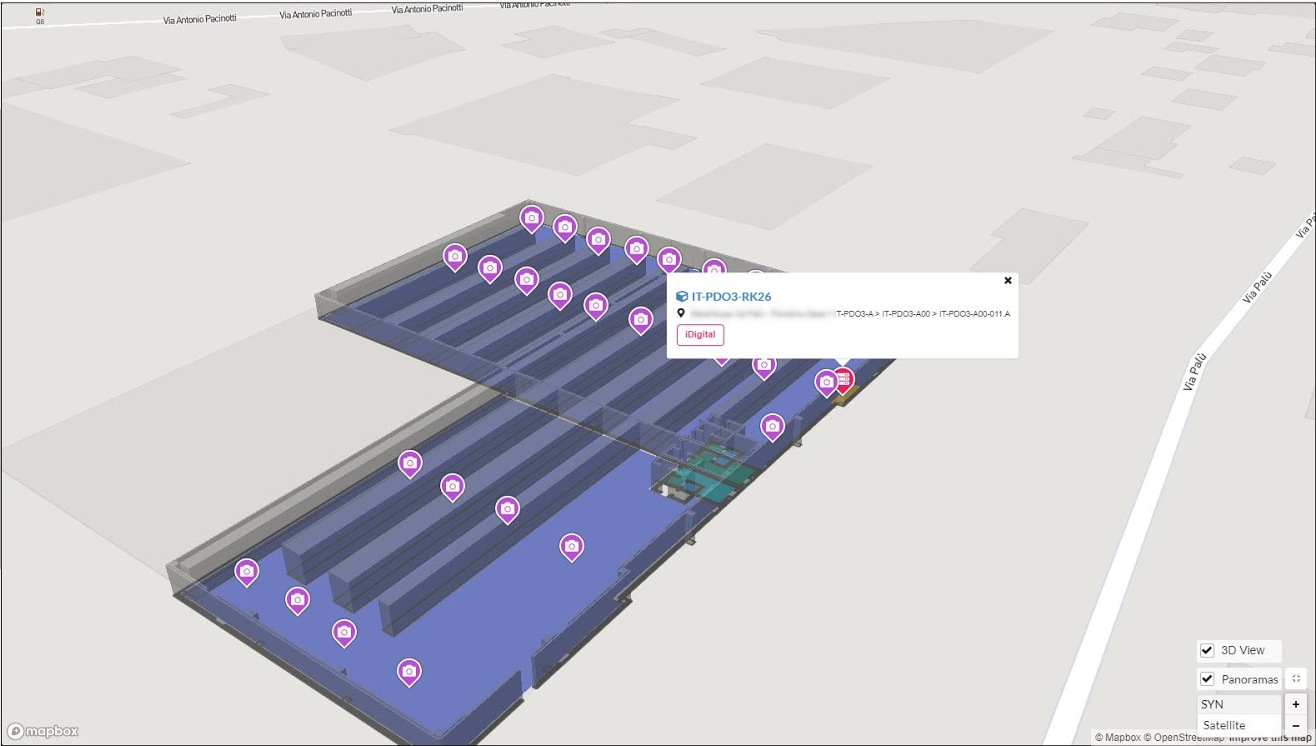
\includegraphics[height=5cm]{datasoil_assets_3dmap}
    \caption{Visualizzazione 3D di impianto produttivo con \textit{asset} mappati. Fonte: \href{https://datasoil.it/industry-40-smartcity-syn-asset-performance/auditing-inventory/}{Datasoil}}
\end{figure}
L'obiettivo è manipolare ed elaborare dati di natura inerentemente caotica, ordinarli e presentarli all'utente finale tramite interfacce grafiche intuitive (impiegando tecnologie all'avanguardia sia lato \textit{frontend} che lato \textit{backend}\footnote{\textit{Fronted} e \textit{backend} denotano, rispettivamente, la parte visibile all'utente di un programma e con cui egli può interagire (tipicamente un'interfaccia utente) e la parte che permette l'effettivo funzionamento di queste interazioni. {\tiny Fonte: \href{https://it.wikipedia.org/wiki/Front-end_e_back-end}{Wikipedia}}}).
\begin{figure}[H]
    \centering
    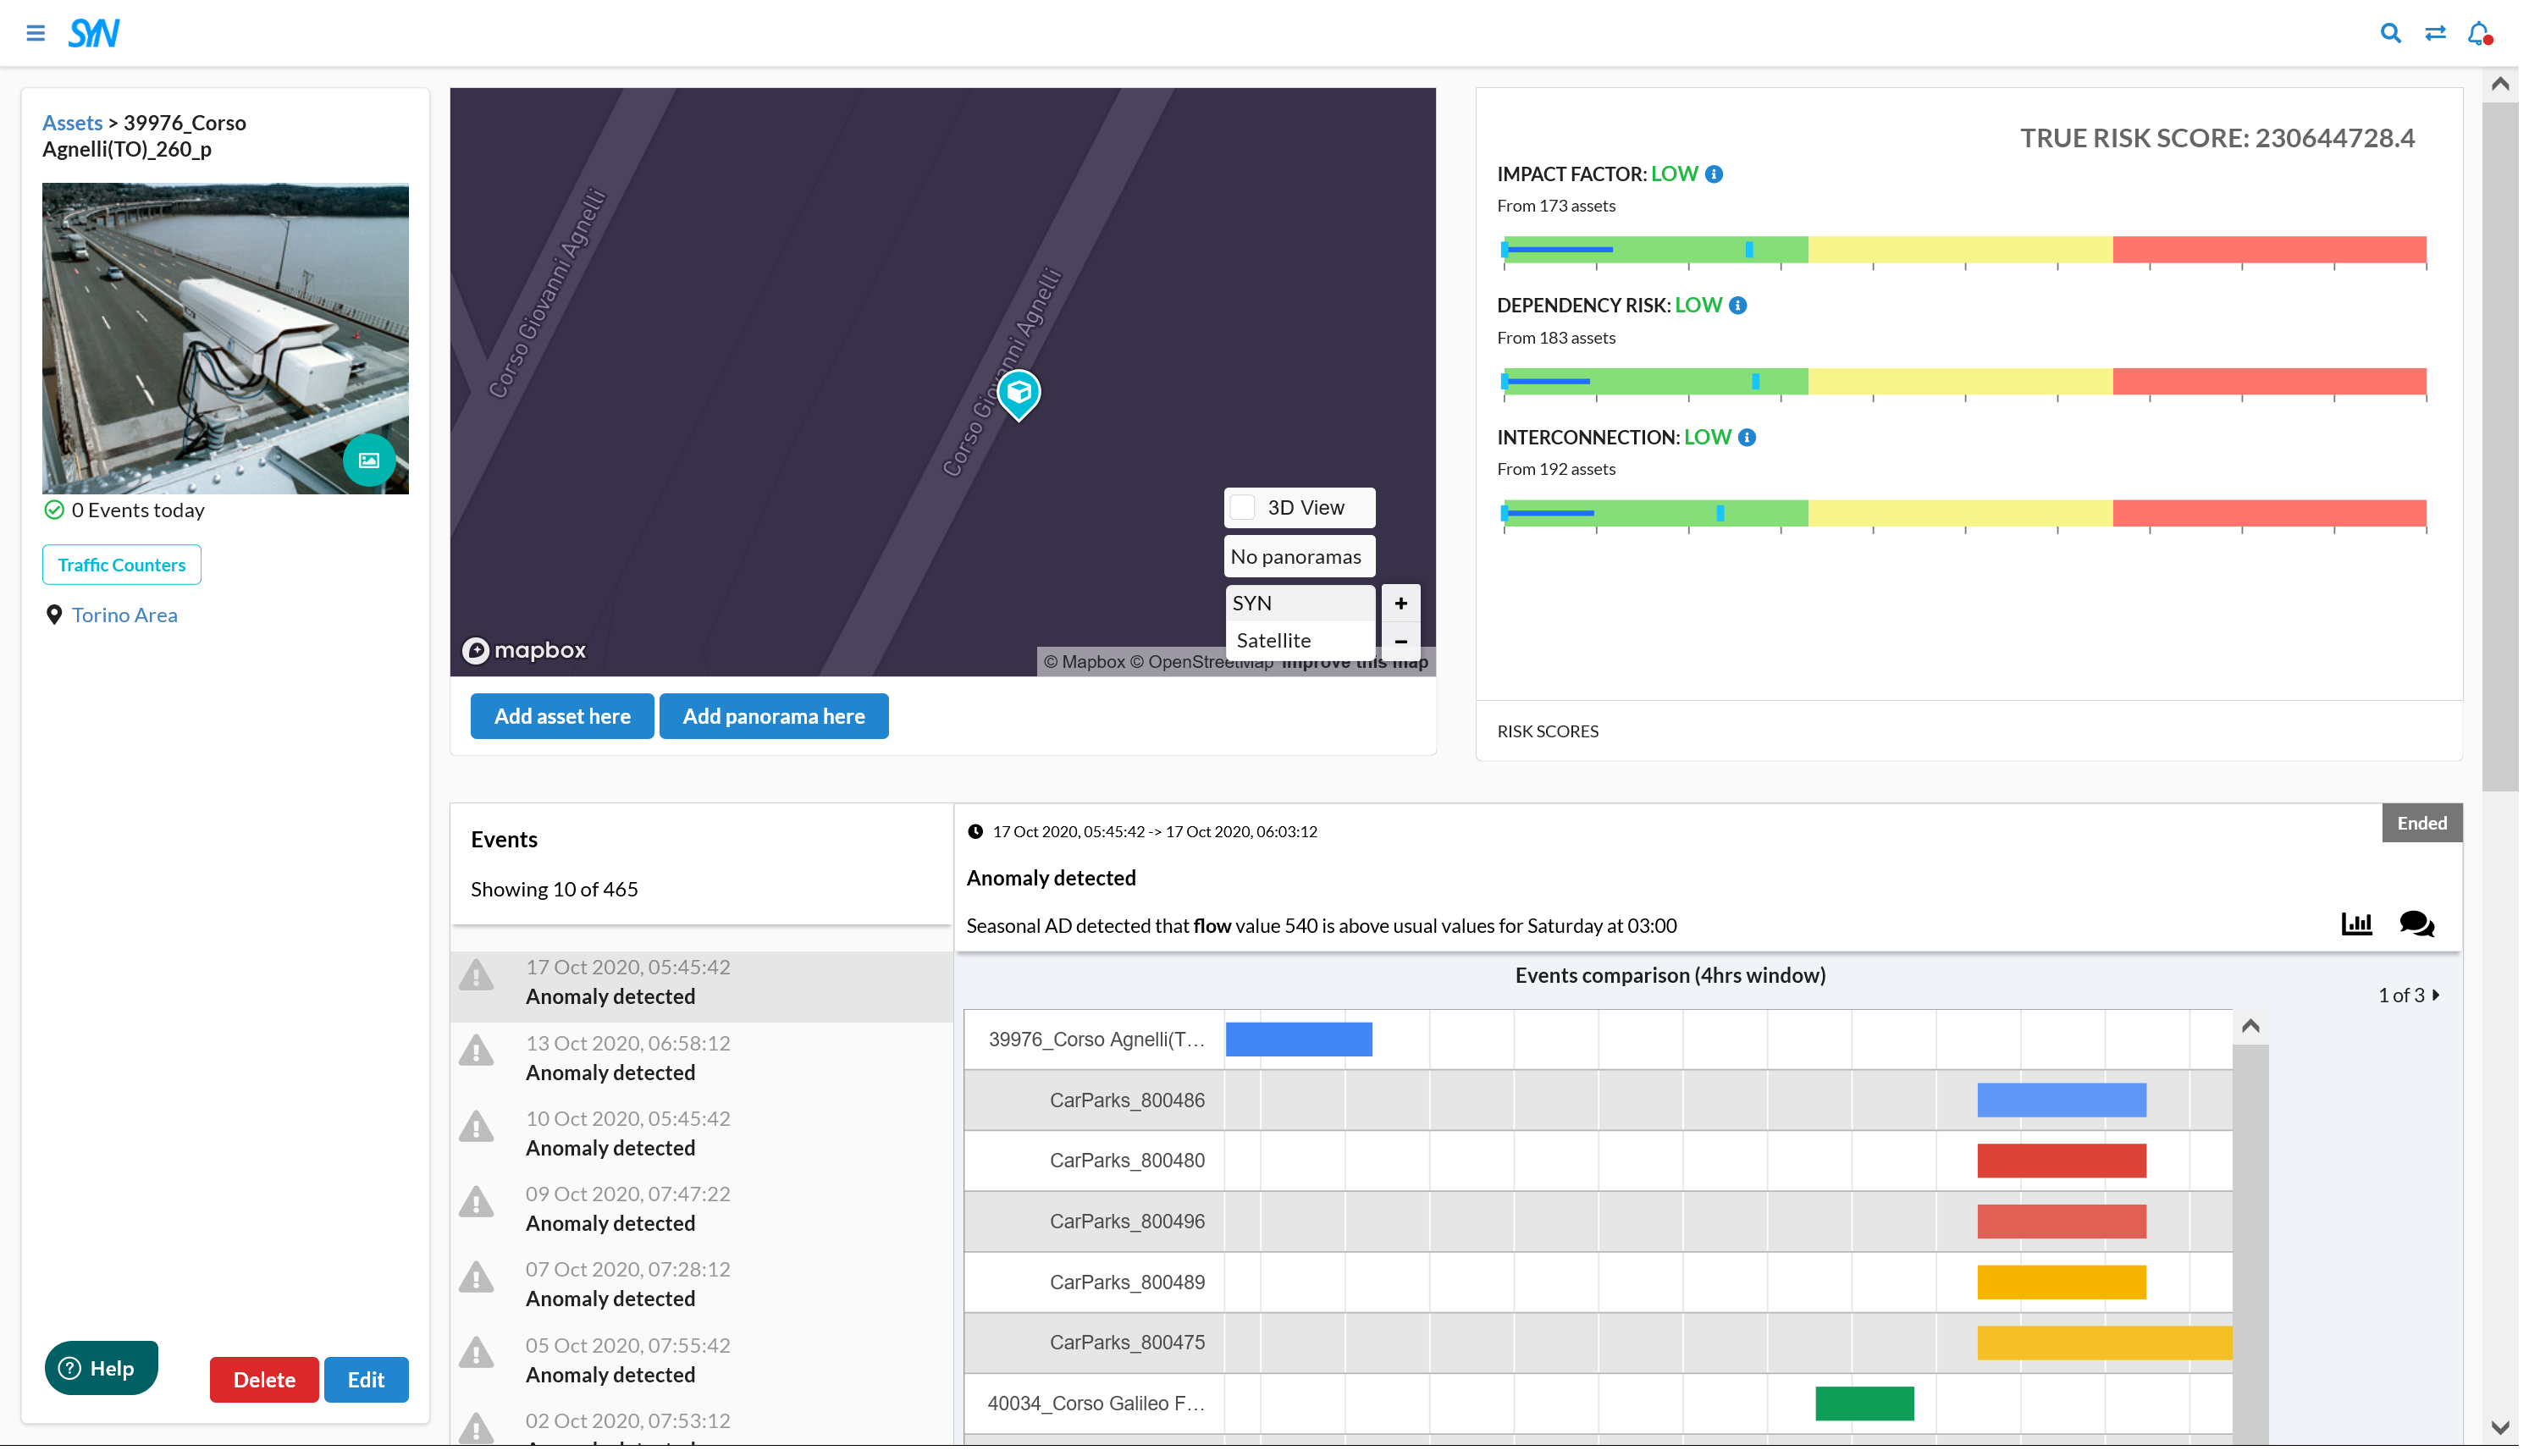
\includegraphics[width=\textwidth]{metriche_asset_datasoil}
    \caption{\textit{Screenshot} visualizzazione grafica di metriche di controllo per \textit{asset} aziendale.}
\end{figure}
Ho avuto modo di verificare molte di queste affermazioni direttamente tramite il progetto proposto, in quanto si tratta di un applicativo legato all'industria 4.0 che mappa \textit{asset} aziendali (come ad esempio macchinari) a un gemello digitale, permettendo sia di localizzarli su una mappa tridimensionale sia, obiettivo dello stage, di visualizzarli in realtà aumentata.

\subsection{Clientela}
\begin{figure}[H]
    \centering
    \includegraphics[height=5.5cm]{screenshot_home_datasoil}
    \caption{L'immagine scelta dall'azienda per il proprio sito mostra una chiara direzione aziendale. Fonte: \href{https://datasoil.it/industry-40-smartcity-syn-asset-performance/}{Datasoil}}
\end{figure}
Si evince da quanto discusso nella sezione precedente che l'offerta di Datasoil sia indirizzata a una clientela professionale, o meglio, aziendale, piuttosto che al mondo \textit{consumer}: 
l'applicazione sulla quale ho svolto lo Stage (MobileSYN) si occupa di gestione e controllo per \textit{asset} aziendali, e un altro prodotto da loro sviluppato, chiamato LifestyleSync, fornisce strumenti di monitoraggio della salute dei dipendenti, con \textit{app} di supporto "LSCoach" che permette a un allenatore di preparare allenamenti personalizzati e verificarne il progresso.\\
In sintesi Datasoil si focalizza su aziende industriali \textit{asset intensive} (ovvero con molti macchinari), manifatturiere e petrolifere, come ad esempio \href{https://www.stevanatogroup.com/it/}{Stevanato Group}.

\subsection{Processi interni}
L'azienda si serve di servizi noti e standardizzati per organizzare il lavoro e la comunicazione interna, ovvero Slack per la messaggistica, Meet per la comunicazione vocale a distanza, Jira per gestire il tracciamento delle \textit{issue} ("cose da fare" in ambito \textit{software}) e facilitare meccanismi agili di integrazione continua, e infine GitHub per quanto riguarda il controllo di versione.\\
Durante il progetto di stage che, per sua natura, è altamente sperimentale e ha quindi richiesto un approccio \textit{"trial and error"} ci si è limitati a usare una piccola Kanban Board di Jira per pianificare, per quanto possibile, il lavoro da svolgere.\\
L'azienda adotta un sistema di lavoro agile (come accennato sopra sfruttando Jira per applicare \textit{continuous delivery}) e fornisce anche ad associazioni esterne \textit{tutoring} riguardo a queste tematiche. 
\begin{figure}[H]
    \centering
    
\includegraphics[width=\textwidth]{continuous-delivery-pipeline}
    \caption{\textit{Continuous delivery pipeline} tramite Jira. Fonte: \href{https://www.atlassian.com/continuous-delivery}{Atlassian}}
\end{figure}

%************************************************************************************************************
\section{Tecnologie e strumenti}
\label{sec:tecnologie-e-strumenti}
Di seguito vengono riportate le tecnologie e gli strumenti utilizzati durante il corso dello stage, divisi in due macrocategorie: di sviluppo (quindi legati strettamente alla produzione di \textit{software}) e organizzativi (più interessati alla gestione del codice prodotto e la comunicazione interna).\\
Verranno prima presentati singolarmente e in dettaglio, per poi mostrarne una visione d'insieme.

\subsection{Tecnologie e strumenti di sviluppo}
\subsubsection{Visual Studio Code}
\vsc{} è un \textit{editor} per codice sorgente, sviluppato da Microsoft servendosi del \textit{framework} Electron, disponibile per Windows, Linux e macOS. Le sue funzionalità comprendo supporto per \textit{debugging}, \textit{syntax highlighting}, \textit{intelligent code completion}, \textit{code refactoring}, e integrazione con Git. \\
Gli utenti possono configurare tema, \textit{macro}, preferenze e installare estensioni che ne aumentano le funzionalità aggiungendo ad esempio il supporto ai maggiori linguaggi di programmazione attualmente presenti.\\
Nella "Stack Overflow 2021 Developer Survey", \vsc{} è risultato essere l'IDE più popolare, adottato dal 70\% degli intervistati. {\tiny Fonte: \href{https://en.wikipedia.org/wiki/Visual_Studio_Code}{Wikipedia}}\\
E' inoltre presente e molto comoda l'estensione di Flutter che, tra le altre cose, permette di gestire direttamente nell'interfaccia i vari dispositivi (\textit{smartphone}, \textit{browser} o emulatore) sui quali installare e lanciare l'applicazione che si sta programmando.

\subsubsection{Android Studio}
\astudio{} è l'IDE (\textit{Integrated Development Environment}, ovvero un \textit{software} per facilitare la scrittura di codice) ufficiale del sistema operativo di Gooogle, sostituendo Eclipse dal 2015, costruito sul \textit{software} IntelliJ di JetBrains e progettato specificatamente per lo sviluppo Android. E' disponibile per Windows, Linux e macOS.\\
Il 7 maggio 2019 Kotlin rimpiazzò Java come linguaggio consigliato per Android, favorendo un'integrazione ancora maggiore con JetBrains che, appunto, ha sviluppato e prodotto Kotlin stesso.\\
Personalmente ho cercato nonostante tutto di programmare il più possibile su \vsc{} preferendolo quindi ad \astudio{} in virtù della sua maggiore leggerezza e delle sue più ampie possibilità di personalizzazione.

\subsubsection{Xcode}
Xcode è l'\ide{} per macOS, utilizzato obbligatoriamente per sviluppare \textit{software} per macOS, iOS, iPadOS, watchOS e tvOS.\\
Supporta codice sorgente i seguenti linguaggi: C, C++, Objective-C, Objective-C++, Java, AppleScript, Python, Ruby, ResEdit (Rez), e Swift (quest'ultimo è per noi di particolare interesse).\\
In generale è un \ide{} molto impopolare e viene percepita con grande frustrazione la sua obbligatorietà per lo sviluppo all'interno dell'ecosistema Apple. Personalmente mi sento allineato alla negativa opinione generale, complice soprattutto la scarsa responsività del programma.


\subsubsection{Dart}
Dart è un linguaggio di programmazione sviluppato da Google per il \textit{client development}, ovvero per applicazioni \textit{web} e \textit{mobile}, e può anche essere impiegato per la costruzione di applicazione \textit{desktop} e \textit{server}.\\
E' un linguaggio orientato agli oggetti, basato su classi, \textit{garbage-collected}, fortemente tipizzato e con una sintassi nello stile di C. Può compilare sia codice macchina che JavaScript e supporta interefacce, \textit{mixins}, classi astratte, \textit{refined generics} e inferenza di tipo.\\
Personalmente l'ho trovato elegante e conciso nella sua struttura, e presenta dei vantaggi consistenti come le espressioni ternarie e la \textit{null safety} (ovvero i valori di tipo \textit{null} devono essere esplicitati con sintassi specifiche che riducono enormemente la possibilità di incontrare errori a tempo di esecuzione).

\subsubsection{Flutter}
Flutter è un \textit{framework open-source} creato da Google per lo sviluppo dell'interfaccia utente di applicazioni multipiattaforma per Android, iOS, Linux, macOS, Windows, Google Fuchsia e il \textit{web} partendo da un singolo \textit{codebase} (collezione di \textit{file} sorgente necessari a ottenere un \textit{software} completo e funzionante).\\
Rilasciato a maggio 2017, le applicazioni in Flutter sono scritte in Dart e sfruttano molte delle funzionalità avanzate del linguaggio. Le componenti principali del \textit{framework} sono:
\begin{itemize}
    \item \textbf{Dart platform:} Flutter gira all'interno della Dart Virtual Machine, che si serve di un \textit{execution engine just-in-time};
    \item \textbf{Flutter engine:} scritto primariamente in C++, fornisce supporto a basso livello per il \textit{rendering} e implementa accessibilità, \textit{file} e \textit{network input/output}, supporto nativo per i \textit{plugin} e molto altro;
    \item \textbf{Foundation library:} scritta in Dart, fornisce classi e funzioni di base che vengono usate per costruire gli applcativi in Flutter, come ad esempio le \textit{Application Programming Interfaces} per la comunicazione con l'\textit{engine};
    \item \textbf{Design-specific widgets:} Flutter contiene due famiglie di \textit{widget} che si conformano a delle specifiche scuole di \textit{design}: "Material" per Google e "Cupertino" per Apple;
    \item \textbf{Flutter DevTools:} famiglia di strumenti generici che vengono sfruttati per lo sviluppo di \textit{software} in Flutter.
\end{itemize}
~\\
Inoltre, una libreria fondamentale per semplificare l'utilizzo di Flutter è "Flutter Hooks": lo scopo è implementare delle strutture simili agli Hooks di React, che consentono di sostituire gli "Stateful Widget" riducendo la quantità di codice ripetuto e semplificando la gestione del ciclo di vita dei \textit{widget} grazie alla funzione "useEffect".

\subsubsection{Java}
Java è un linguaggio di programmazione ad alto livello orientato agli oggetti progettato per avere il minor numero possibile di dipendenze implementative (favorendo quindi l'uso di interfacce e classi astratte) e, soprattutto, per aderire al motto \textit{"write once, run anywhere"}: il \textit{bytecode} di Java può infatti girare senza necessità di ricompilazione su qualsiasi piattaforma che supporti la Java Virtual Machine (comunemente abbreviata in JVM).\\  
La sintassi è simile a quelle di C o C++, ma fornisce funzionalità dinamiche generalmente inedite per i linguaggi compilati, come \textit{reflection} (un programma in esecuzione può modificare se stesso) e modifica del codice a \textit{runtime}.\\
Originalmente rilasciato nel 1995 come componente centrale della piattaforma Java per Sun Microsystems e sotto licenza proprietaria, dal 2007 la maggior parte dei suoi componenti sono diventati \textit{open-source} sotto l'ombrello della "GPL-2.0-only" (licenza specifica per \textit{software} libero pubblicata dalla Free Software Foundation).\\
Sebbene Oracle (attuale proprietario di Sun Microsystems) offra un'implementazione proprietaria chiamata "HotSpot JVM", la specifica ufficiale è la "OpenJDK JVM" che è gratuita, \textit{open-source} e predefinita nella maggior parte delle distribuzioni Linux.

\subsubsection{Kotlin}
Kotlin è un linguaggio di programmazione multipiattaforma staticamente tipizzato. Progettato per avere completa interoperabilità con Java, gode di una sintassi più concisa di quest'ultimo grazie all'inferenza di tipo di cui è dotato. Dipende dalla Java Class Library per la versione della Java Virtual Machine da usare.\\
E' inoltre in grado di compilare codice in JavaScript (sfruttato poi da applicazioni \textit{frontend}) o codice nativo tramite "LLVM" (per app iOS che condividono le logiche operative con applicazioni Android).\\
Incluso in Android Studio come alternativa al compilatore standard Java dal 2017, produce \textit{bytecode} Java 8 di default ma permette al programmatore di scegliere delle versioni successive (fino a Java 18).

\subsubsection{Swift}
Swift è un linguaggio di programmazione ad alto livello, compilato, sviluppato da Apple e dalla comunità \textit{open-source}.\\
Inizialmente rilasciato nel 2014, il suo scopo è rimpiazzare il precedente linguaggio di Apple Objective-C, ormai obsoleto visto che è rimasto largamente invariato dagli anni '80 ed è quindi manchevole di funzionalità moderne.\\
Swift lavora con i \textit{framework} Cocoa e Cocoa Touch, e un aspetto chiave del suo \textit{design} è l'interoperabilità con una grossa parte del codice esistente in Objective-C (che, naturalmente, permea l'ecosistema Apple) sfruttando la \textit{runtime library} di Objective-C (che permette anche di far girare C e C++).\\
E' stato costruito con il \textit{framework} di compilazione LLVM ed è stato incluso in Xcode dalla sesta versione, rilasciata nel 2014.

\subsubsection{Azure Spatial Anchors}
Azure Spatial Anchors è un servizio di Microsoft mirato a fornire strumenti per sviluppare applicazioni in realtà aumentata su dispositivi iOS o Android predisposti per, rispettivamente, ARKit e ARCore, oppure su Microsoft HoloLens.\\
Permette di riconoscere spazi tridimensionali all'interno dei quali posizionare punti di interesse, chiamati Spatial Anchors, che possono essere salvati in \textit{cloud} e poi recuperati, e possono essere messi in relazione a oggetti reali (come macchinari in un contesto industriale) o virtuali.

\subsubsection{ARCore}
ARCore, conosciuto anche come Google Play Services per AR, è un \sdk{} (generalmente abbreviato in SDK) prodotto da Google per permettere lo sviluppo di applicazioni in realtà aumentata.\\
Si serve di tre componenti principali:
\begin{itemize}
    \item \textbf{6DOF:} il dispositivo sfrutta una piattaforma inerziale a sei assi per comprendere e tracciare la propria posizione relativa allo spazio;
    \item \textbf{Environmental understanding:} permette riconoscere dimensioni e locazione delle superfici lisce;
    \item \textbf{Light estimation:} permette al telefono di stimare le condizioni di luce dell'ambiente.
\end{itemize}
\asa{} si appoggia proprio ad ARCore per implementare le proprie funzionalità di realtà aumentata su Android.

\subsubsection{ARKit}
ARKit è la controparte Apple di ARCore, ovvero è un \sdk{} che permette lo sviluppo di applicazioni in realtà aumentata su dispositivi Apple.\\
Combina i dati del dispositivo di tracciamento spaziale (come la piattaforma inerziale a sei assi) con un \textit{processing} avanzato della scena ripresa per fornire un'esperienza in realtà aumentata convincente.\\
Indubbiamente migliore di ARCore, produce risultati più fluidi (inteso come effettiva fluidità percepita guardando la scena attraverso il dispositivo), meglio implementati con le tecnologie esistenti e risparmia al programmatore molti oneri (come la gestione delle sessioni) occupandosene direttamente in modo autonomo.

\subsubsection{Visione d'insieme}
\vsc{} è un \textit{editor} per codice sorgente che permette grande estensibilità tramite \textit{plugin} appositi che, per il progetto, ho configurato in modo tale da aggiungerci la compatibilità con il \textit{framework} utilizzato per lo sviluppo \textit{mobile}, ovvero Flutter, che si appoggia sul linguaggio Dart. Quest'ultimo è un linguaggio orientato agli oggetti e fortemente tipizzato che nasce per la creazione di interfacce grafiche \textit{frontend mobile}. Integrando Flutter in \vsc{} si ottengono vari vantaggi, come ad esempio la possibilità di gestire eventuali emulatori o dispositivi Android con facilità.\\
Essendo lo scopo del progetto l'integrazione di \asa{} (tecnologia per gestire ancoraggi in realtà aumentata) in un'applicazione Flutter, è stato necessario studiare anche gli \sdk{} sui quali si appoggia il servizio di Microsoft, ovvero ARCore (lato Android) e ARKit (lato iOS). \asa{} implementa tali funzionalità in linguaggi nativi, ovvero Java per Android e Swift per iOS, il che ha portato la necessità a utilizzare due \ide{}(abbreviato in IDE) ulteriori a \vsc{}: Xcode e Android Studio.\\
Xcode è obbligatorio per programmare in Swift, mentre Android Studio da un grosso aiuto al programmatore quando lo usa per sviluppare applicazioni Android in Java o Kotlin (linguaggio che si è dovuto utilizzare per \aplug{}, ovvero il \textit{framework} ultimamente selezionato che tratteremo nel terzo capitolo di questo documento).
\begin{figure}[H]
    \textbf{Strumenti di sviluppo e rispettivi linguaggi:}
    \begin{center}
    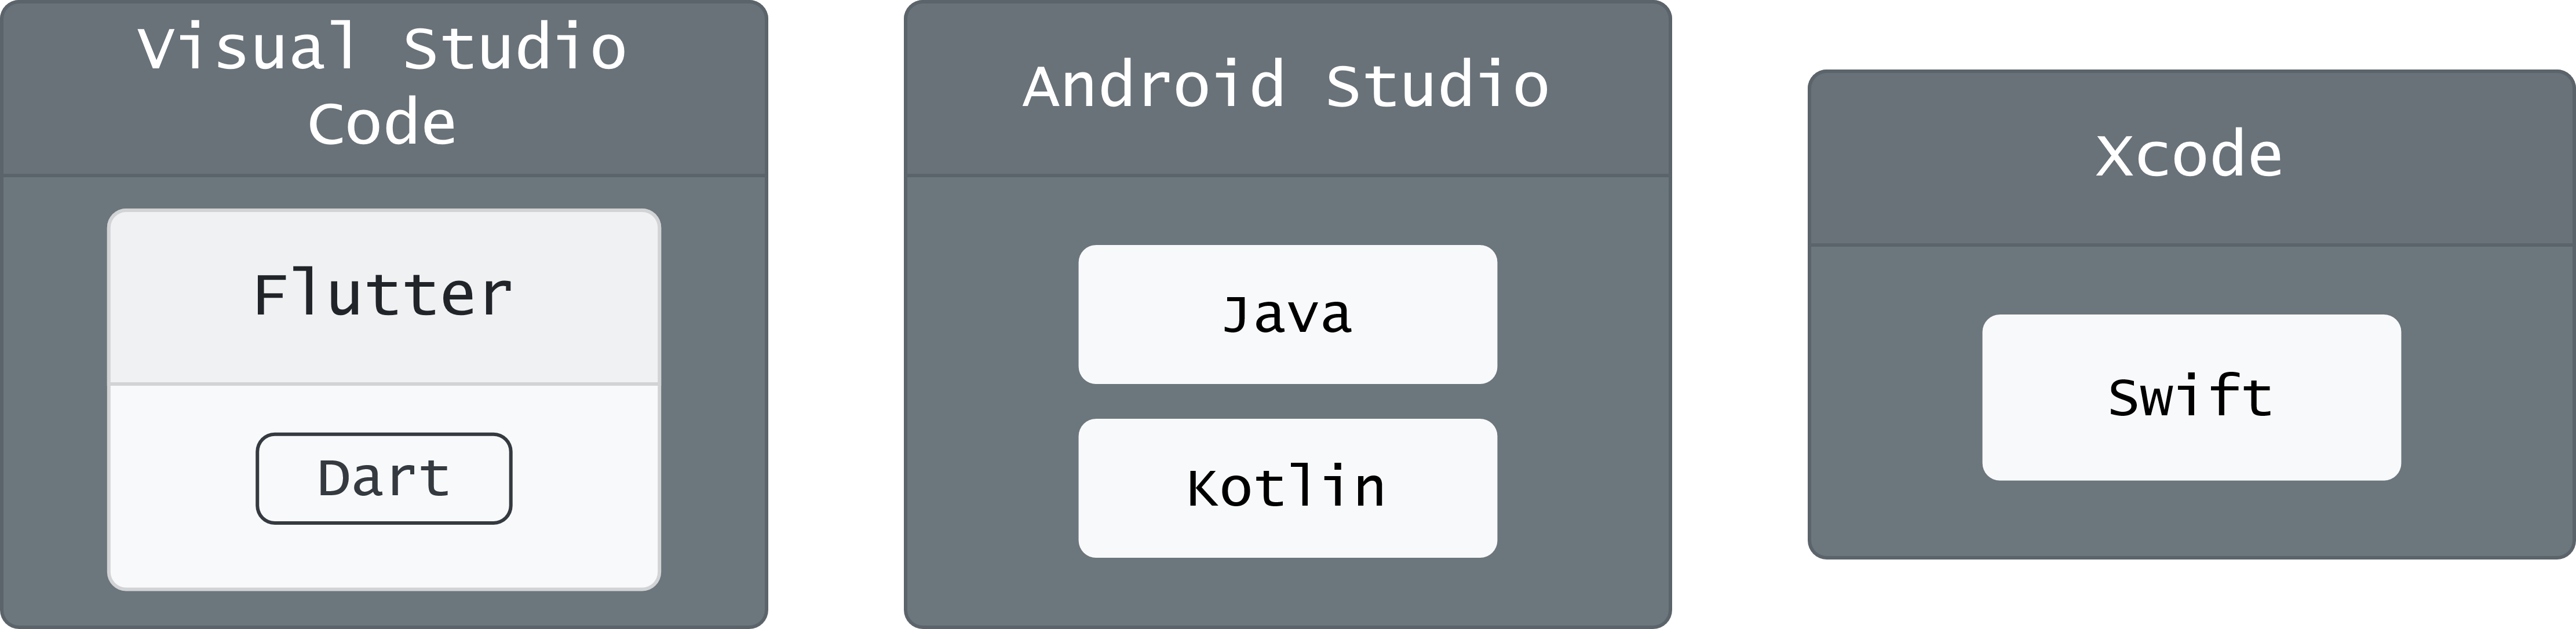
\includegraphics[height=3cm]{ides}
    \caption{\textit{Integrated development environments} e linguaggi per i quali sono stati usati}
    \end{center}
\end{figure}

\begin{figure}[H]
    \textbf{Tecnologie realtà aumentata, linguaggi e sistemi operativi:}
    \begin{center}
    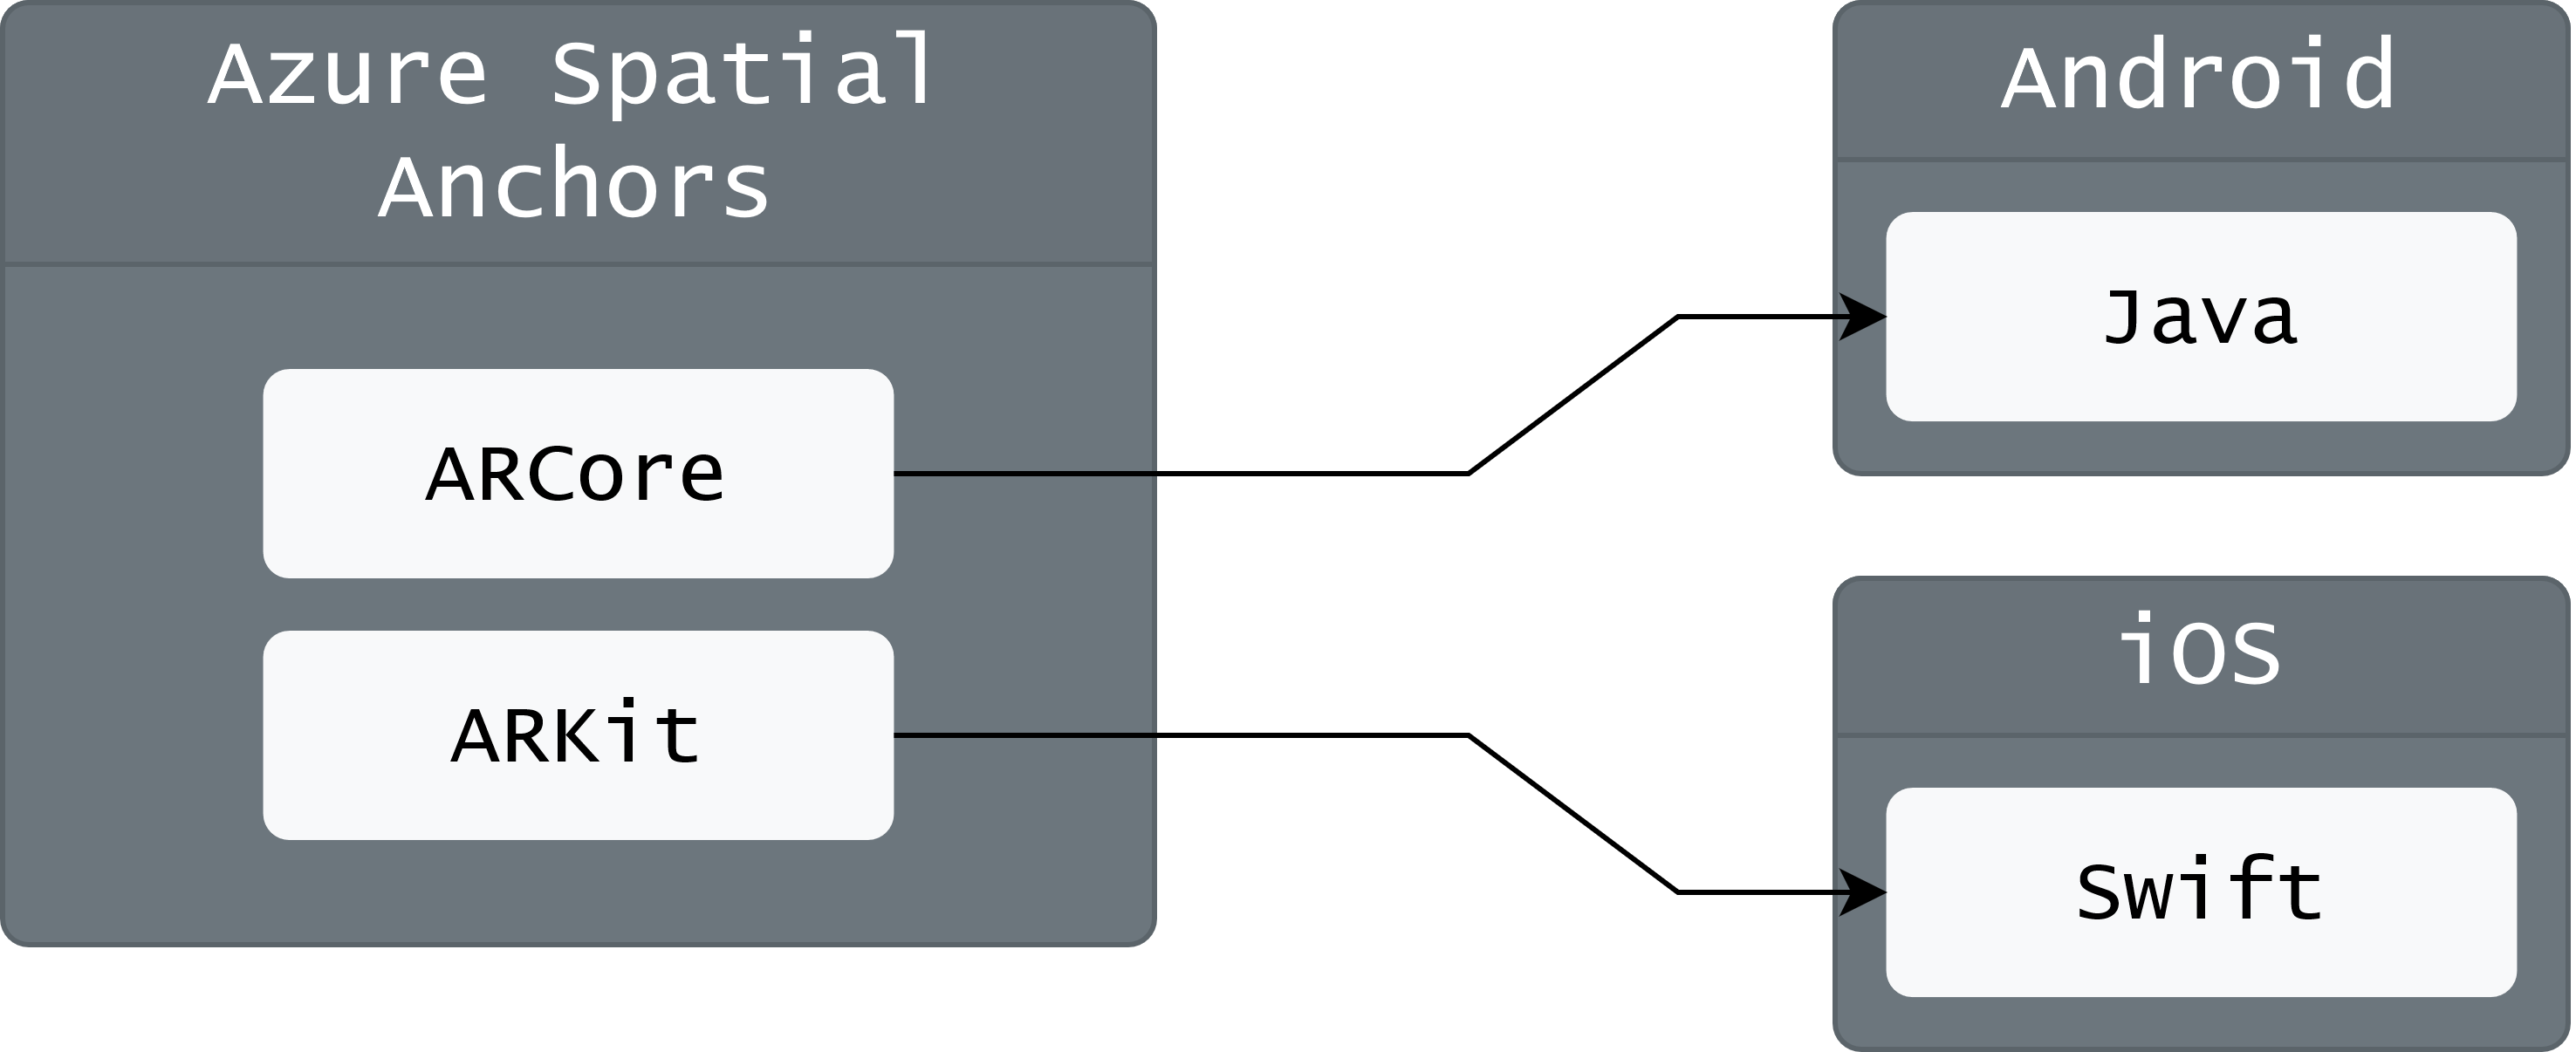
\includegraphics[height=3.5cm]{tecASA}
    \caption{\asa{} e linguaggi nativi utilizzati per implementare le sue componenti in Android e iOS}
    \end{center}
\end{figure}

\begin{figure}[H]
    \textbf{\textit{Framework} scelto e sua relazione con tecnologie e linguaggi:}\\
    In questo caso il \textit{framework} ha le componenti native scritte in Kotlin che è compatibile nativamente con Java e funge quindi da contenitore (\textit{"wrapper"}) per quest'ultimo.\\
    \begin{center}
    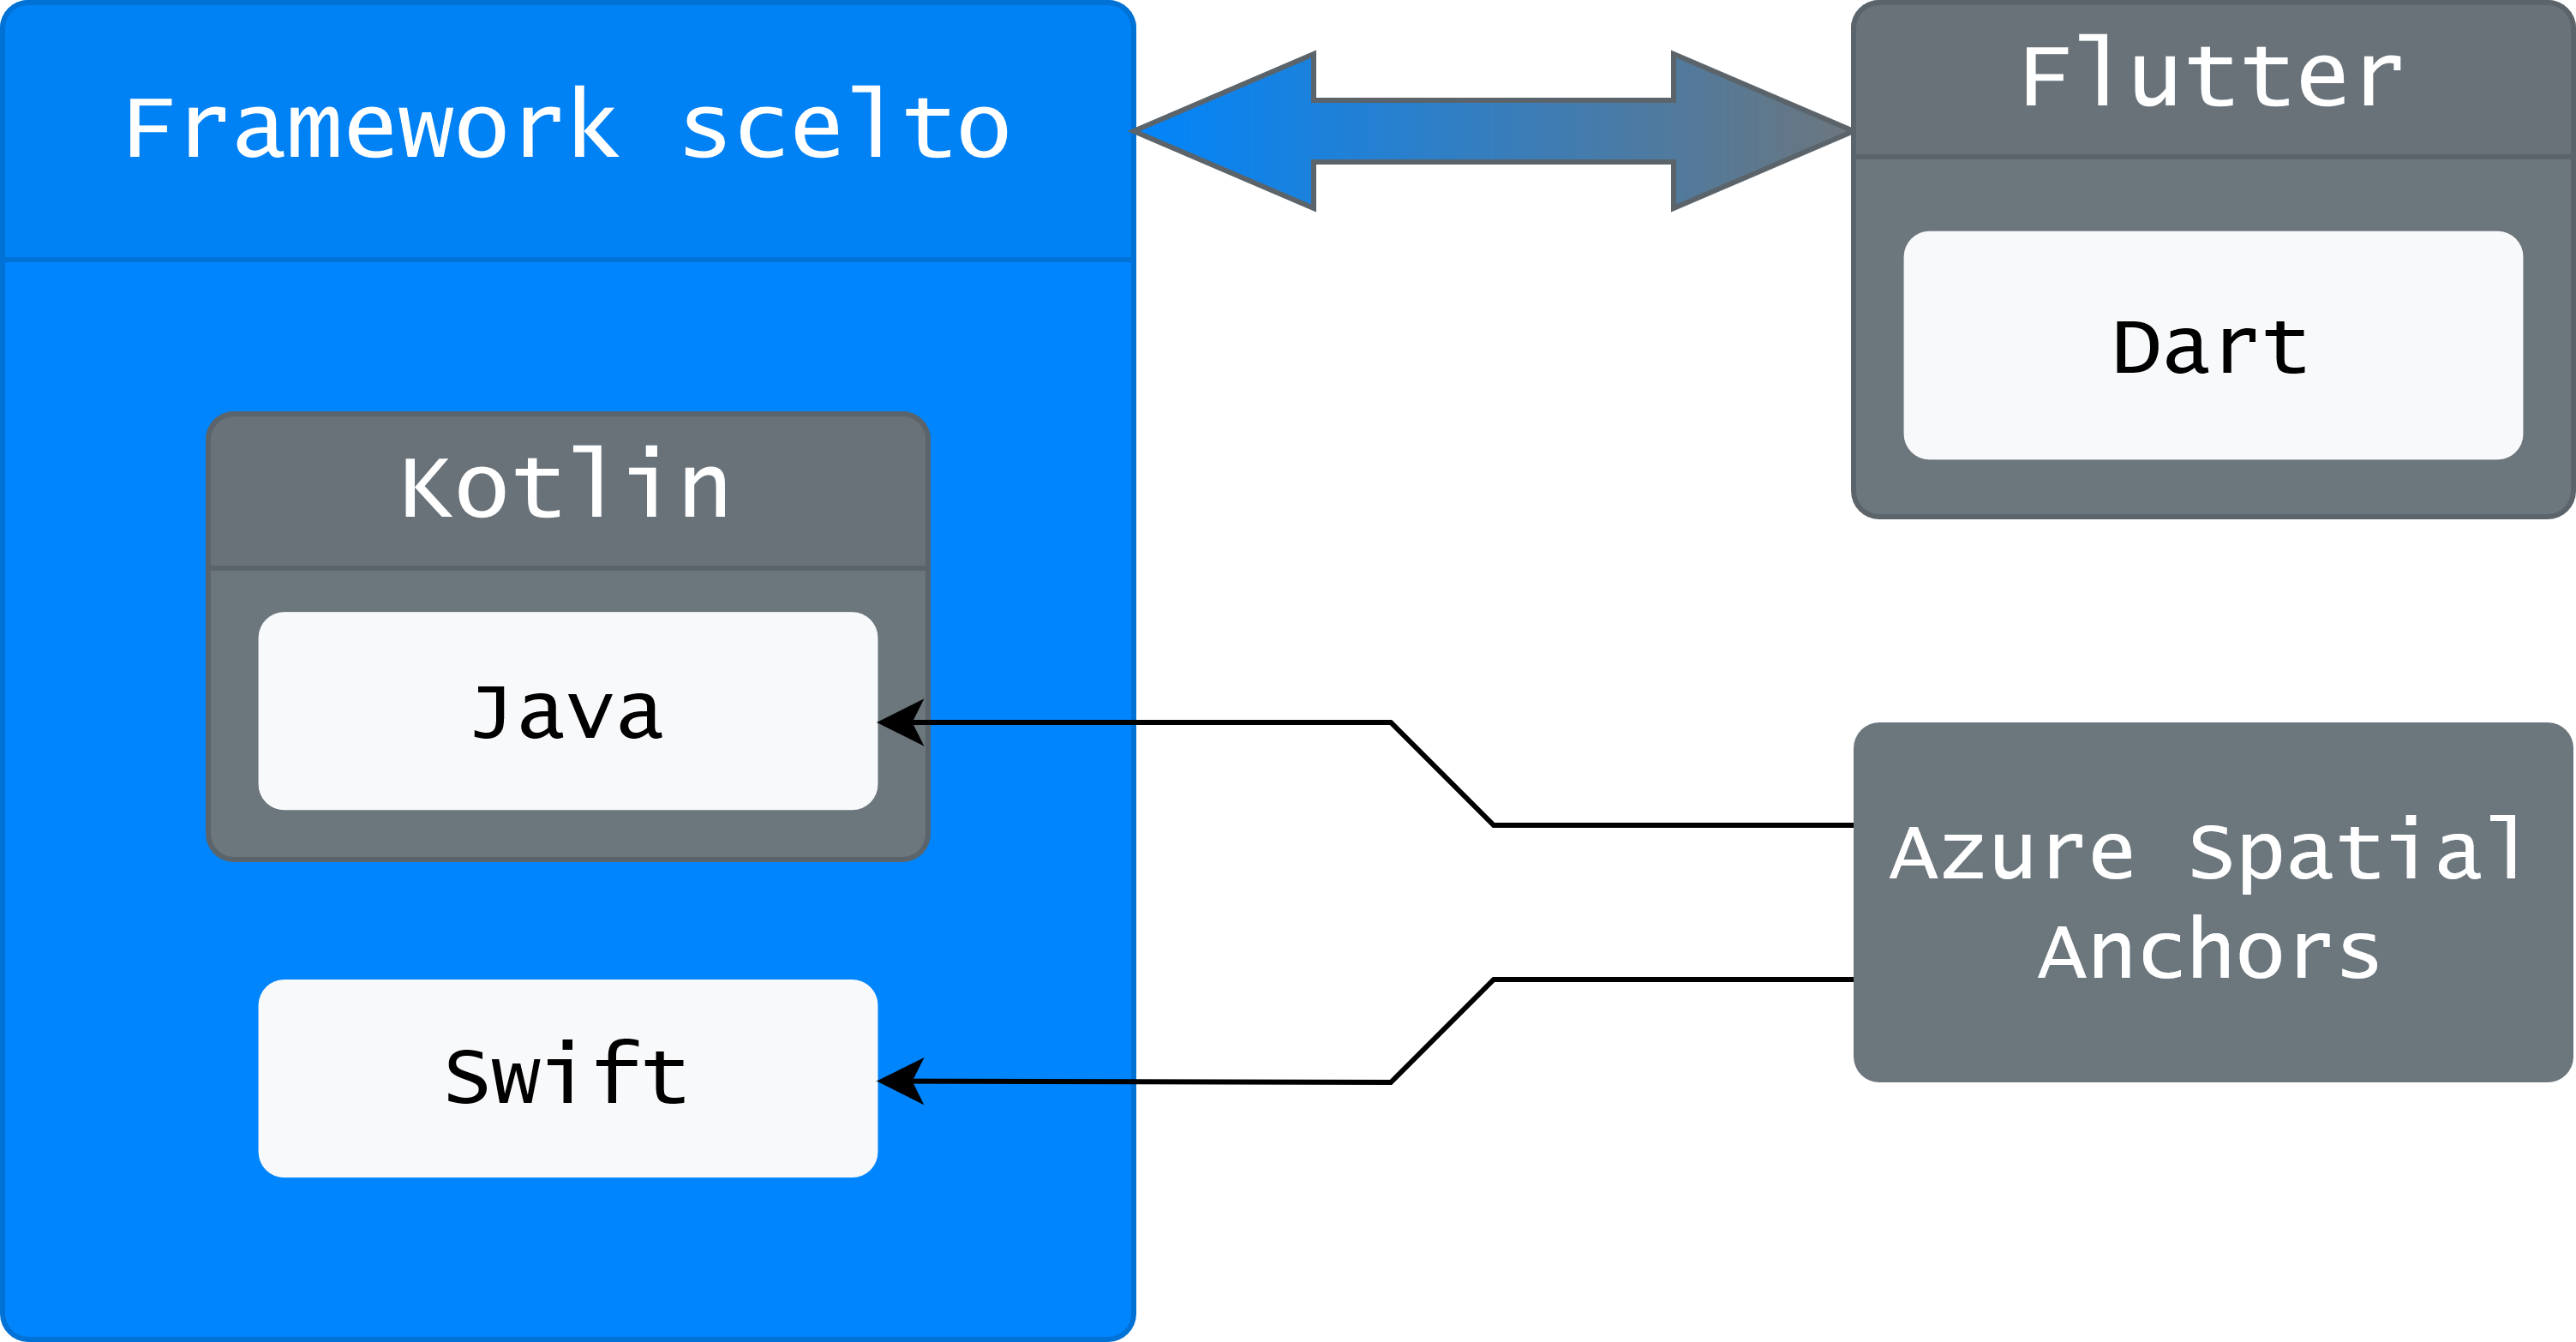
\includegraphics[height=4.5cm]{aplug_linguaggi}
    \caption{Il \textit{framework} selezionato comunica con Flutter e implementa delle componenti native alle quali si interfacciano le \asa{}}
    \end{center}
\end{figure}
%**************************************************************
\subsection{Strumenti organizzativi}
\subsubsection{Slack}
Slack è una piattaforma di comunicazione istantanea di proprietà di Salesforce e sviluppata da Slack Technologies per Windows, Linux, macOS, Android e iOS.\\
Permette di comunicare tramite messaggi, chiamate vocali e video, e di inviare \textit{media} e \textit{files} nelle \textit{chat} private o nei canali. Quest'ultimi fungono da aggregatori e permettono di suddividere tematicamente la comunicazione.\\
E' inoltre possibile suddividere a un livello ancora più alto tramite i \textit{workspaces}, che aggregano al proprio interno utenti, canali e applicazioni: sono proprio quest'ultime che mostrano con maggiore chiarezza l'orientamento aziendale di Slack, che infatti fornisce integrazione nativa con i maggiori software gestionali e organizzativi (come ad esempio Jira, Zoom, Drive, Outlook, etc).

\subsubsection{Github}
GitHub è il più grande servizio di \textit{hosting} di codice sorgente al mondo, abitualmente usato per sviluppare progetti \textit{open-source}, e fornisce vari servizi: controllo di versione tramite Git distribuito e \textit{access control}, \textit{bug tracking}, \textit{issue tracking}, richieste di modifiche \textit{software}, \textit{task management}, integrazione continua e \textit{wiki} per ogni progetto.\\ 
Permette inoltre, tramite \textit{forking}, \textit{pull request} e commenti, il miglioramento collaborativo del \textit{software}, ad esempio risolvendo errori, aggiungendo funzionalità o migliorando quelle presenti.

\subsubsection{Jira}
Jira è un \textit{software} proprietario sviluppato da Atlassian che si occupa di fornire una piattaforma potente e funzionale di \textit{bug} e \textit{issue tracking}, presentando il tutto tramite interfacce grafiche chiare e complete. Favorisce inoltre la pianificazione e la collaborazione all'interno dei \textit{team} utilizzando, oltre alle \textit{issues}, anche \textit{tasks} e \textit{user stories}.\\
Fornisce inoltre \textit{template} già pronti per implementare i più noti \textit{framework} di lavoro come Scrum e Kanban.\\
Jira mira inoltre a ottimizzare il flusso di lavoro e favorire un miglioramento continuo fornendo visualizzazioni espressive di metriche per tenere traccia dei tempi di sviluppo e scoprire colli di bottiglia.

\subsubsection{Visione d'insieme}
Presentiamo ora gli strumenti organizzativi in relazione tra loro e con quelli di sviluppo, assieme a descrizione minimale. Per approfondire i singoli elementi si rimanda alle sezioni immediatamente successive.\\
Per quanto riguarda la comunicazione diretta interna all'azienda, che sia condividere documenti, frammenti di codice o domande di vario tipo, lo strumento scelto è Slack (piattaforma di messaggistica orientata alle aziende).\\
Tutto il codice per tutte le tecnologie affrontate (applicazione MobileSYN, esempi ufficiali \asa{}, \textit{framework} selezionato) è contenuto in GitHub, che fornisce sia \textit{hosting} che controllo di versione. Infine per organizzare quanto possibile i lavori si è scelto di utilizzare Jira (\textit{software} proprietario di \textit{issue tracking}), che è anche integrato in Slack.\\
\begin{figure}[H]
    \centering
    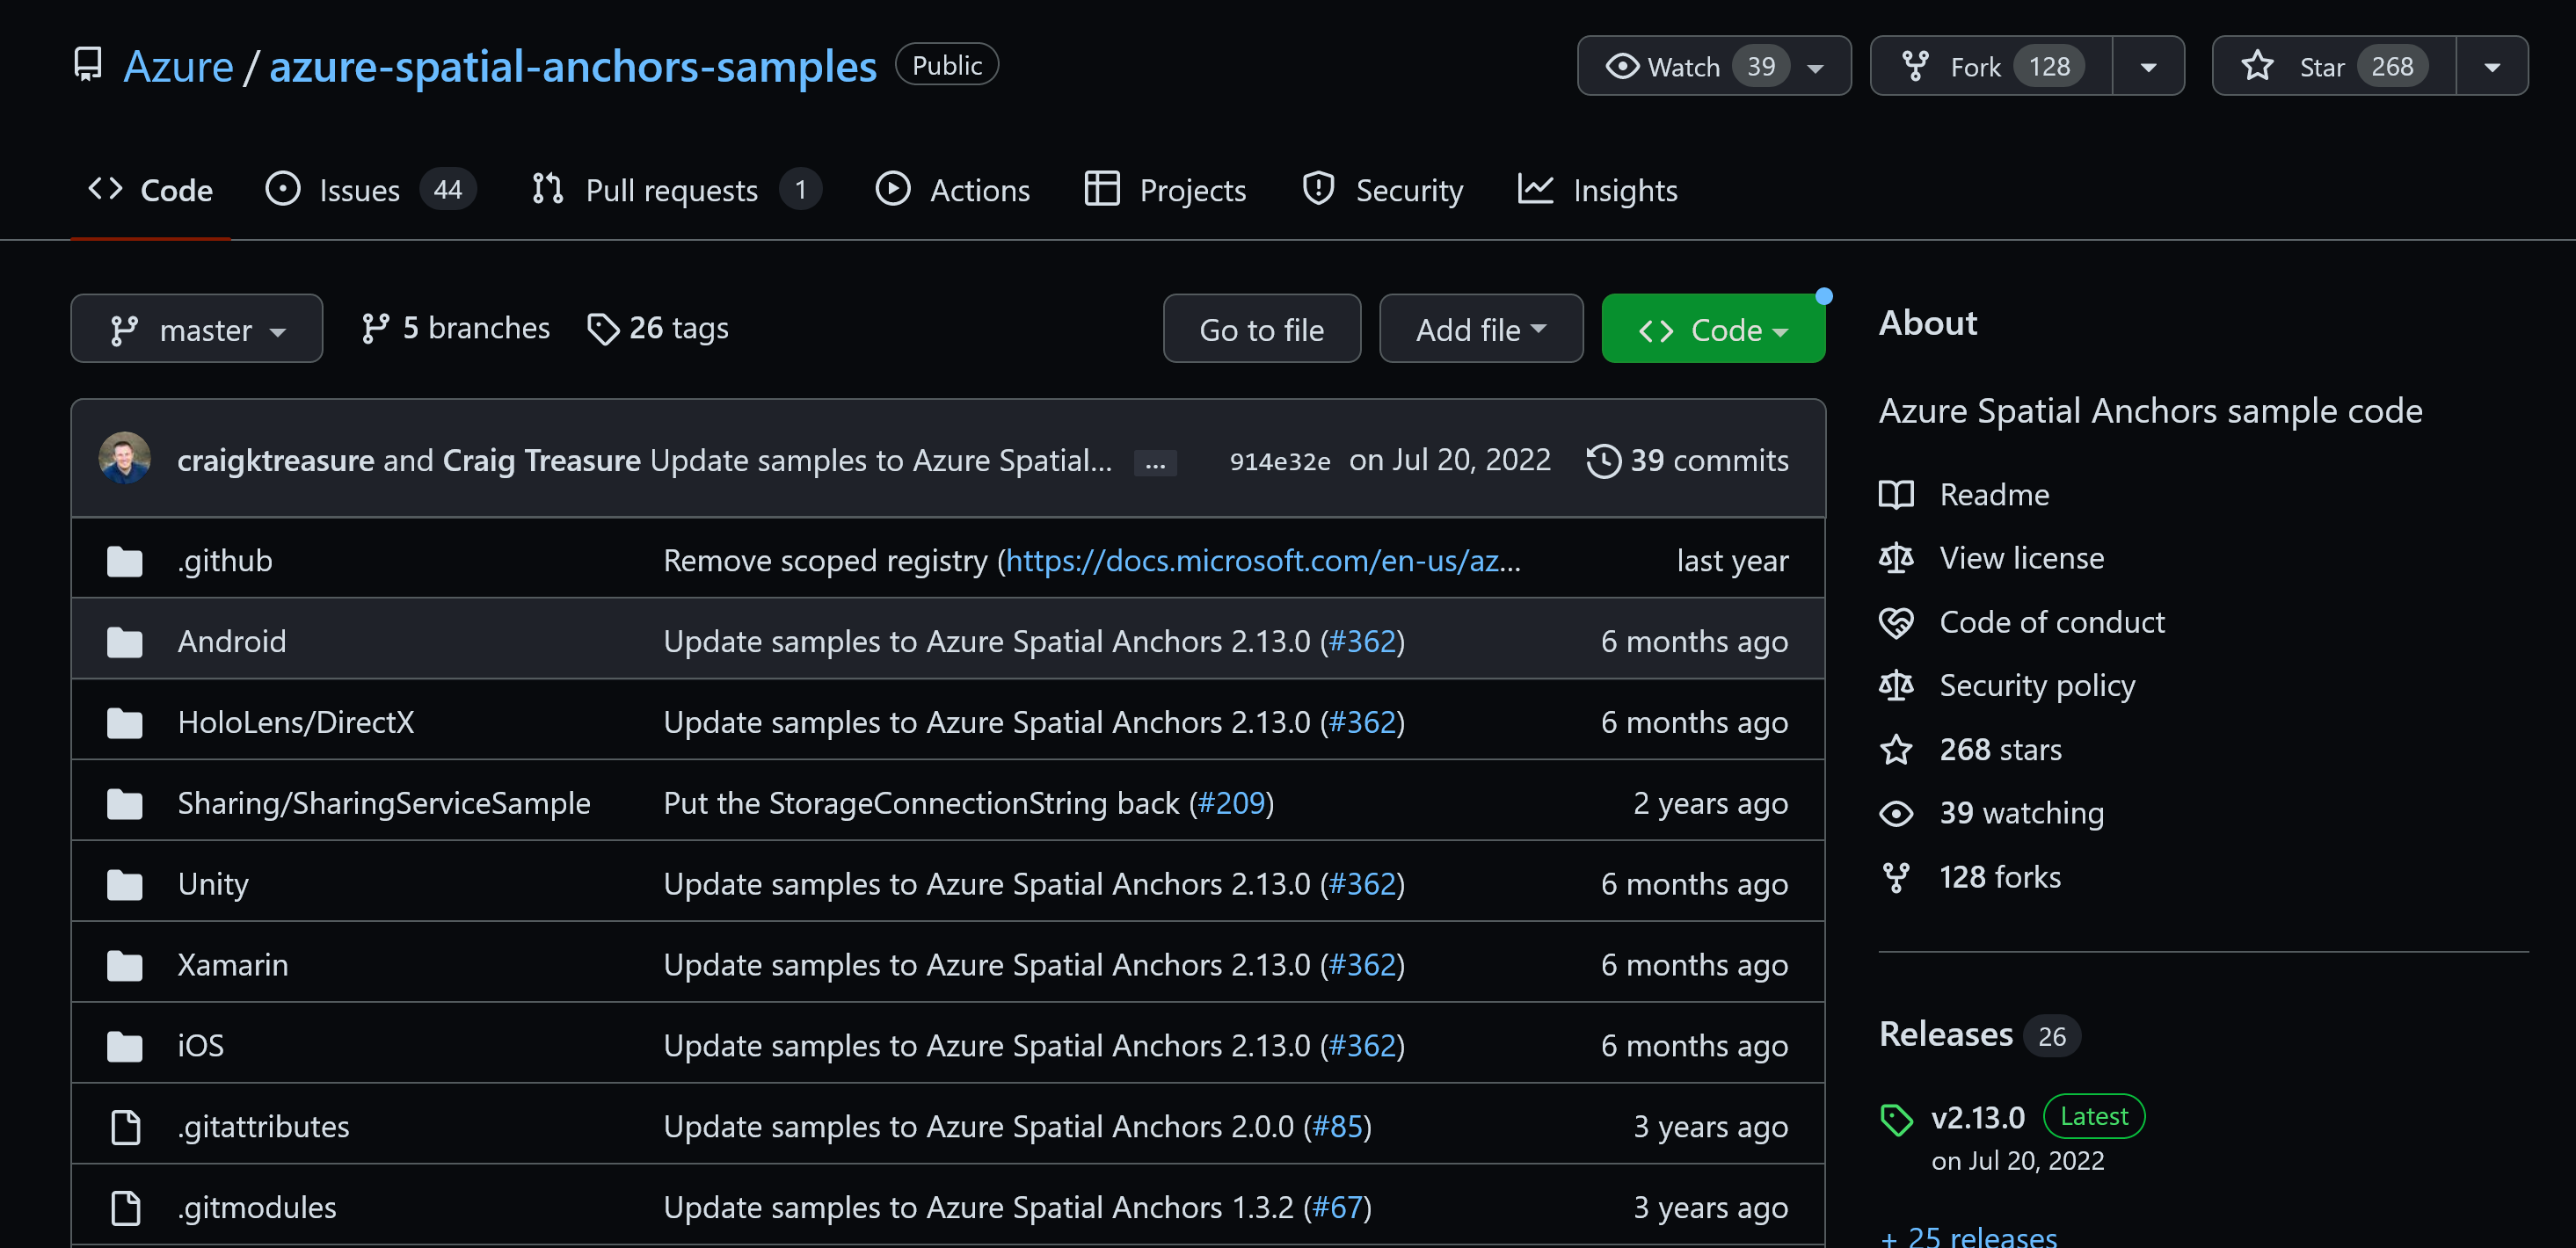
\includegraphics[width=\textwidth]{asa_github_screen}
    \caption{Il codice per l'applicazione di esempio ufficiale di \asa{} è interamente contenuta in \href{https://github.com/Azure/azure-spatial-anchors-samples}{questa} \textit{repository} di GitHub}
\end{figure}

\section{Innovazione, stage e prodotti}
E' immediatamente evidente guardando le tecnologie impiegate che Datasoil pone particolare attenzione sul tema dell'innovazione: lato \textit{backend} troviamo servizi \aws{} impiegati per decentralizzare la gestione del \textit{server} (ad esempio S3), e ovviamente il già citato \asa{}, mentre lato \textit{frontend}\footnote{Collezione di codice che fornisce funzionalità generiche che possono essere sovrascritte, specializzandole, per adattarle agli scopi voluti. Sono simili alle librerie se visti come astrazioni riutilizzabili di codice incluso in APIs (\textit{Application Programming Interfaces}, permettono a due o più componenti \textit{software} di comunicare) ben definite, tuttavia ciò che le differenzia è che il controllo di esecuzione non è dettato dal chiamante, ma dal \textit{framework} stesso. E' proprio questa inversione di controllo la caratteristica principale dei \textit{framework}.} vediamo l'impiego di linguaggi di programmazione e \textit{framework} recenti come Dart e Flutter (usati per sviluppare tutt i prodotti in campo \textit{mobile}).\\
E' bene sottolineare, però, che gli strumenti scelti non sono stati selezionati solo per rincorrere un ideale di avanguardia: hanno infatti tutti alle spalle delle grosse corporazioni (Amazon nel caso di \aws{}, Microsoft nel caso di \asa{} e Google nel caso di Dart e Flutter) che garantiscono loro un certo grado di stabilità e sicurezza.\\
L'attenzione all'innovazione mostrata da Datasoil si riflette sia negli \textit{stage} proposti che nei prodotti e servizi direttamente offerti dall'azienda: ad esempio nell'uso di HoloLens per implementare funzioni di realtà aumentata oppure nelle sessioni di \textit{tutoring} per terzi (riguardo appunto queste tecnologie o pratiche di sviluppo agile) che i \textit{senior} svolgono a cadenza regolare.
\begin{figure}[H]
    \centering
    \begin{minipage}{.5\textwidth}
      \centering
      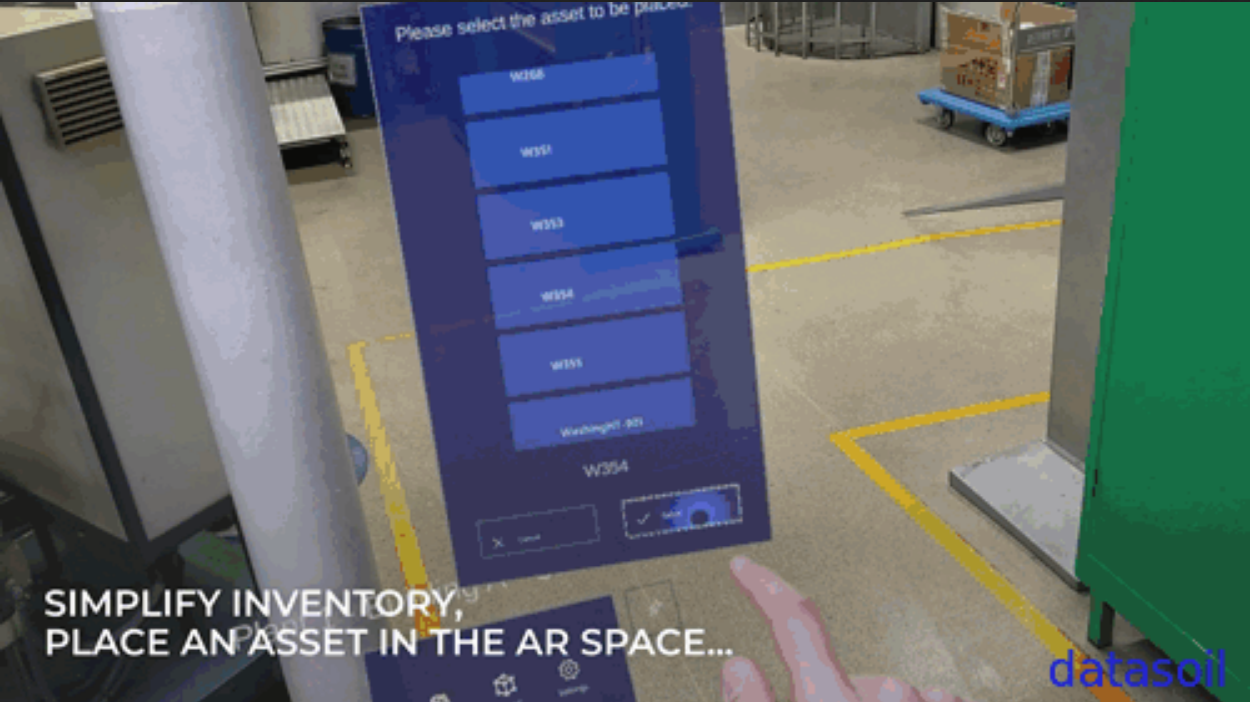
\includegraphics[width=1\linewidth]{hololens1_datasoil}
      \captionof{figure}{Menù HoloLens}
      \label{fig:test1}
    \end{minipage}%
    \begin{minipage}{.5\textwidth}
      \centering
      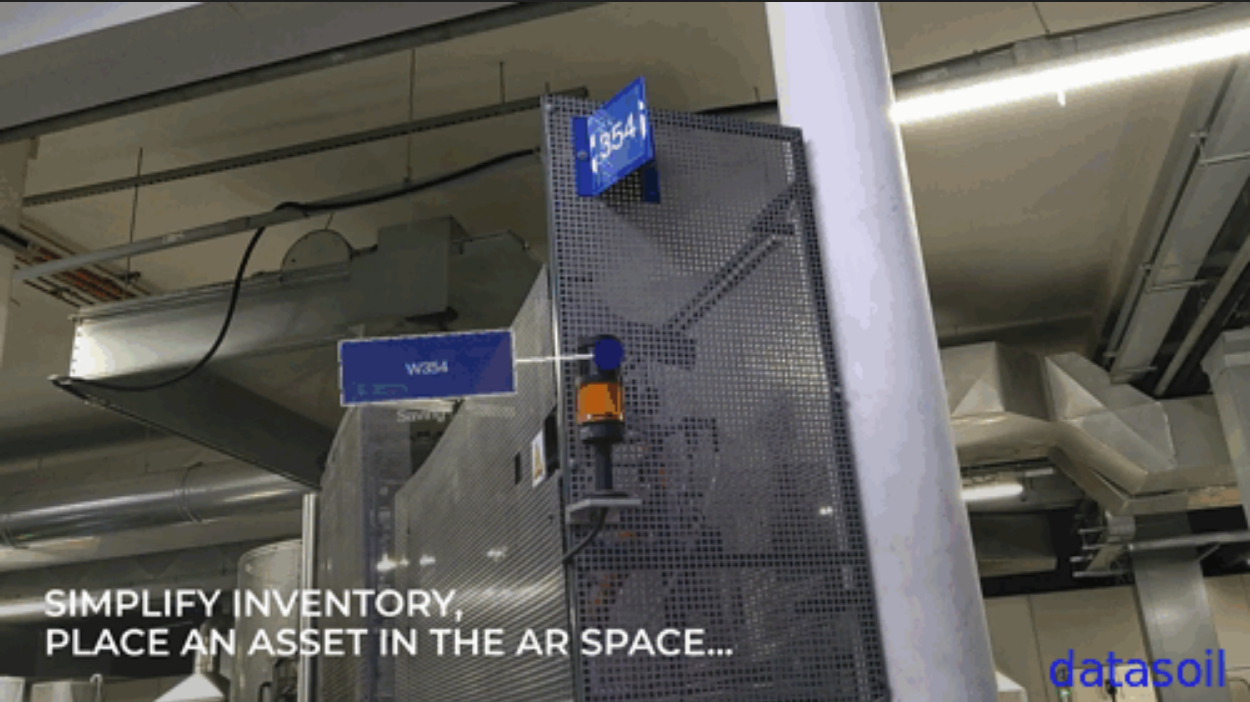
\includegraphics[width=1\linewidth]{hololens2_datasoil}
      \captionof{figure}{Posizionamento \textit{asset}}
    \end{minipage}
    \caption{HoloLens usato in azienda per gestire \textit{asset} in realtà aumentata. Fonte: \href{https://datasoil.it/industry-40-smartcity-syn-asset-performance/auditing-inventory/}{Datasoil}}
\end{figure}
Gli \textit{stage} riescono a essere innovativi sia direttamente che indirettamente: se si tratta di un progetto sperimentale vero e proprio lo è per sua stessa natura, tuttavia anche nel caso in cui l'obiettivo sia limitato a sviluppare funzioni in maniera più "meccanica", porta comunque lo studente ad avere a che fare con gli strumenti moderni che vengono impiegati giornalmente in azienda.\\
Vengono quindi integrati nel contesto aziendale in modalità duplice: a volte sono funzionali alla sperimentazione di nuove soluzioni, altre volte sono già inquadrati in una \textit{pipeline} produttiva (ad esempio potrebbero trattare lo sviluppo di alcune pagine di un'applicazione \textit{mobile}). Anche nel primo caso però se ciò che è stato prodotto risulta interessante per dei possibili clienti viene portato avanti e integrato anche quando lo \textit{stage} si è ormai concluso.

% !TEX encoding = UTF-8
% !TEX TS-program = pdflatex
% !TEX root = ../tesi.tex

%**************************************************************
\chapter{Lo Stage}
\label{cap:lo-stage}
%**************************************************************
\section{Descrizione e temi}
Il progetto proposto prevede l'implementazione di una vista in realtà aumentata per l'applicazione di ticketing e monitoraggio aziendale "\textbf{SYN}".\\
La componente AR dovrà necessariamente appoggiarsi al servizio di {asa} perchè gli {asset} aziendali tracciati da \textbf{SYN} hanno un {digital twin} ancorato e localizzato proprio tramite le {anchor} di Microsoft, e dovrà idealmente essere cross-platform quindi fornendo l'implementazione adeguata sia per Android che per iOS.\\
Dalla vista dovrà essere possibile interagire con gli {asset}, quindi ottenendoli dal cloud e presentandoli nella scena AR, e con i ticket a loro associati, provocando l'apparizione di una card all' on-tap dell'{asset}, ovvero mostrando a schermo tramite una lista testuale i vari ticket relativi all'{asset} dopo che questo viene toccato.\\
Per concludere l'interezza degli obiettivi sarà necessario studiare dei {framework} o degli {SDK} che permettono l'integrazione di {asa} in codice nativo (che sarà Java per Android e Swift per iOS) con il {framework} Flutter e il linguaggio su cui si poggia, ovvero Dart.

\section{Strategia aziendale}
\section{Attività a supporto}


\section{Obiettivi}
\begin{itemize}
    \item Minimi:
        \begin{itemize}
            \item Studio e comprensione del linguaggio di programmazione \textit    {Dart} e del {framework} \textit{Flutter};
            \item Analisi toolkit Azure: Azure Console e {asa};
            \item Ricerca di {framework} e {SDK} per implementare le    {asa} in \textit{Flutter};
            \item Eventuale studio di linguaggi ulteriori necessari alle    implementazioni native, come ad esempio \textit{Kotlin}, \textit{Java},    \textit{Unity} o \textit{Swift};
            \item Completamento del {framework} scelto nell'app \textit{Flutter}    esistente;
            \item Completamento dello sviluppo dei componenti per rappresentare le {anchor} nello spazio AR;
            \item Completamento dello sviluppo delle \acrshort{api} per l'interazione utente con le {anchor} AR;
        \end{itemize}
    \item Massimi: 
        \begin{itemize}
            \item Sviluppo di componenti per mappare {asset} aziendali ad {anchor} AR;
            \item Sviluppo di componenti UI per la visualizzazione di metriche e informazioni di controllo.
        \end{itemize}
\end{itemize}

\subsection{Relazione con strategia aziendale}
\section{Vincoli}
\section{Motivazione scelta}

% !TEX encoding = UTF-8
% !TEX TS-program = pdflatex
% !TEX root = ../tesi.tex

%**************************************************************
\chapter{Realizzazione}
\label{cap:realizzazione}
%**************************************************************



\section{Studio delle tecnologie}
\subsection{Flutter}
E' impossibile parlare di Flutter senza prima discutere del linguaggio su cui si basa: Dart.\\
Faremo quindi un'introduzione quanto più sintetica possibile sulle sue caratteristiche più proprietarie, tralasciando invece le similitudini a linguaggi popolari che possono facilmente essere intuite dal lettore.
\subsubsection{Dart}
Dart è un linguaggio compilato fortemente tipizzato con sintassi simile a C, e adotta molte funzionalità tipiche dei linguaggi moderni: considera infatti ogni variabile un oggetto e implementa la \textit{null safety}, obbligando il programmatore a esplicitare con sintassi specifiche la presenza o meno del valore \verb+null+.

\begin{lstlisting}[language=dart, firstnumber=1,caption={Dart \textit{null safety}}]
    //dichiarazione di variabili
    String variabileNotNullable = '';  //non puo' mai essere null
    String? variabileNullable = null;  //puo' anche essere null

    //utilizzo esplicito di variabile nullable
    fun (variableNullable);   //compile error
    fun (?variableNullable);  //esplicito che puo' essere nulla

    //utilizzo esplicito di variabile not nullable
    if (value != null)
        fun (!value);   //dico al compilatore che sono certo value non sia null
\end{lstlisting} 

Permette inoltre l'interpolazione di stringhe:

\begin{lstlisting}[language=dart, firstnumber=1,caption={Dart interpolazone stringhe}]
    //sfrutto il simbolo $
    'number = $variableName';              //inserisco in stringa direttamente una variabile
    'expressionResult = ${expression}';    //inserisco in stringa direttamente un'espressione
\end{lstlisting}

Dart tratta in maniera particolare le funzioni, che sono oggetti, hanno un tipo (\verb+Function+), possono avere parametri posizioni o nominali, obbligatori od opzionali: 

\begin{lstlisting}[language=dart, firstnumber=1,caption={Dart parametri funzioni}]
    //parametri obbligatori posizionali
    void fun (int a, int b);  //non possono essere nulli, non essendo 'int? a'

    //possono essere anteceduti da parametri posizionali opzionali
    void fun (int a, int b, [String opz1 = '', String opz2 = '']){}
    void fun (int a, int b, [String? opz1nullable, String? opz2nullable]){}

    //oppure possono essere anteceduti da parametri nominali opzionali
    void fun (int a, int b, {String opz1 = '', String opz2 = ''}){}
    void fun (int a, int b, {String? opz1nullable, String? opz2nullable}){}

    //non possono essere anteceduti da entrambi
    void fun (int a, int b, [String opz1 = ''], {String opz2 = ''}){} //compile error

    //tutti i costruttori in Dart hanno solo parametri nominali
    //di default i parametri nominali sono opzionali
    //possono pero' essere resi obbligatori con la keyword 'required'
    void fun ({required String obb1, required String? obb2, String opz1 = ''}){}
\end{lstlisting}

Esistono le funzioni anonime (largamente sfruttate nei metodi \verb+build+ di Flutter), che possono essere ovviamente passate come argomento ad altre funzioni, essendo oggetti:

\begin{lstlisting}[language=dart, firstnumber=1,caption={Dart funzioni anonime}]
    //prima sintassi
    (){
        //corpo della funzione anonima
    } 

    //seconda sintassi
    () => return_expression

    //assegnamento di funzione anonima ad una variabile
    //ritorna una stringa con un messaggio portato in upper case
    var upperfy = (msg) => '${msg.toUpperCase()}';

    //passaggio di funzione come parametro
    fun (firstValue, () => secondValue);
\end{lstlisting}

Abbiamo delle espressioni condizionali specifiche del linguaggio dalla grande espressività e che quindi vengono largamente usate:

\begin{lstlisting}[language=dart, firstnumber=1,caption={Dart espressioni ternarie}]
    //primo tipo di condizione, detta ternaria
    condizione ? expr1 : expr2;

    //equivale a (in pseudocodice):
    if (condizione == true) return expr1
    else                    return expr2

    //vediamo un esempio
    int? a;               //a==null di default
    a = a==null ? 1 : 0;  //ad 'a' viene assegnato il valore 1 siccome a==null


    //################################
    //secondo tipo di condizione peculiare:
    expr1 ?? expr2;

    //equivale a (in pseudocodice):
    if (expr1 != null) return expr1
    else               return expr2

    //vediamo un esempio
    int? a;      //a==null di default
    a = a ?? 1;  //ad 'a' viene assegnato il valore 1 siccome a==null
\end{lstlisting}

I caratteri \verb+?+ e \verb+!+ sono, come si evince dalle espressioni ternarie e dalla \textit{null safety}, di cruciale importanza in Dart, ed è quindi opportuno vedere ancora qualche esempio del loro utilizzo:

\begin{lstlisting}[language=dart, firstnumber=1,caption={Dart operatori '?' e '!'}]
    list[1]     //accede al secondo elemento della lista

    list.?[1]
    //equivale a (in pseudocodice):
    if (list[1] != null)    return list[1]
    else                    return null

    //##############################

    foo?.bar 
    //equivale a (in pseudocodice):
    if (foo.bar != null)    return foo.bar
    else                    return null

    //##############################

    foo!.bar
    //equivale a (in pseudocodice):
    if (foo.bar != null)    return foo.bar
    else                    throw (runtimeException)
\end{lstlisting}

Le applicazioni \textit{mobile} e \textit{web} spesso si trovano a eseguire istruzioni che richiedono l'attesa di risorse esterne (ottenere dati dalla rete o leggerli da un \textit{file}, oppure scrivere su un \textit{database}). Per evitare il completo blocco dell'esecuzione (disastroso per un applicativo \textit{consumer}) Dart implementa nativamente delle funzioni di programmazione asincrona, che permetto di svolgere operazioni anche mentre altre sono in attesa.\\
Per fare ciò si serve di tre \textit{keyword}: \verb+async+, \verb+await+ e \verb+Future+:

\begin{lstlisting}[language=dart, firstnumber=1,caption={Dart programmazione asincrona}]
    Future<void> checkVersion () async {
        var version = await lookUpVersion();
    }

    //un'espressione marcata con la keyword 'await' ritorna sempre Future<T>
\end{lstlisting}

Trattiamo infine le caratteristiche peculiari di Dart per quanto riguarda classi e metodi:

\begin{itemize}
    \item Esistono i costruttori costanti, marcati \verb+const+, che sono inizializzati a \textit{compile-time}. Tutti gli altri sono implicitamente dinamici (quindi \textit{run-time});
    \item Posso creare costruttori nominati per implementare costruttori multipli tramite la sintassi:
\begin{lstlisting}[language=dart]
    ClassName.constructorName () :
        firstField = firstValue,
        secondField = secondValue;
\end{lstlisting}
    \item Ogni entità è una classe, ogni classe discende da \verb+Object+ (ad eccezione di \verb+Null+);
    \item Per ogni classe viene creata un'interfaccia implicita che contiene tutti i membri di istanza della classe;
    \item I metodi \textit{getter} e \textit{setter} di una classe vengono creati implicitamente per variabili non \verb+final+, ma possono essere definiti esplicitamente con le \textit{keyword} \verb+get+ e \verb+set+.
\end{itemize}

\subsubsection{Widget}
Mostriamo ora alcuni componenti di Flutter necessari al proseguimento della lettura, partendo dai \textit{widget}: riprendono l'idea di React di costruire tutta l'interfaccia grafica tramite uno \textit{stack} di \textit{widget}, che definiscono il proprio aspetto basandosi sulla configurazione e lo stato attuali. Quando lo stato di un \textit{widget} cambia, esso riscrive la propria descrizione (insieme di istruzioni e valori che lo determinano) e il \textit{framework} valuta le differenze tra questa e la descrizione precedente per apportare le modifiche necessarie al suo \textit{render tree} e quindi, ultimamente, modificarne l'aspetto e finalizzare il cambio di stato.

\begin{figure}[H]
    \centering
    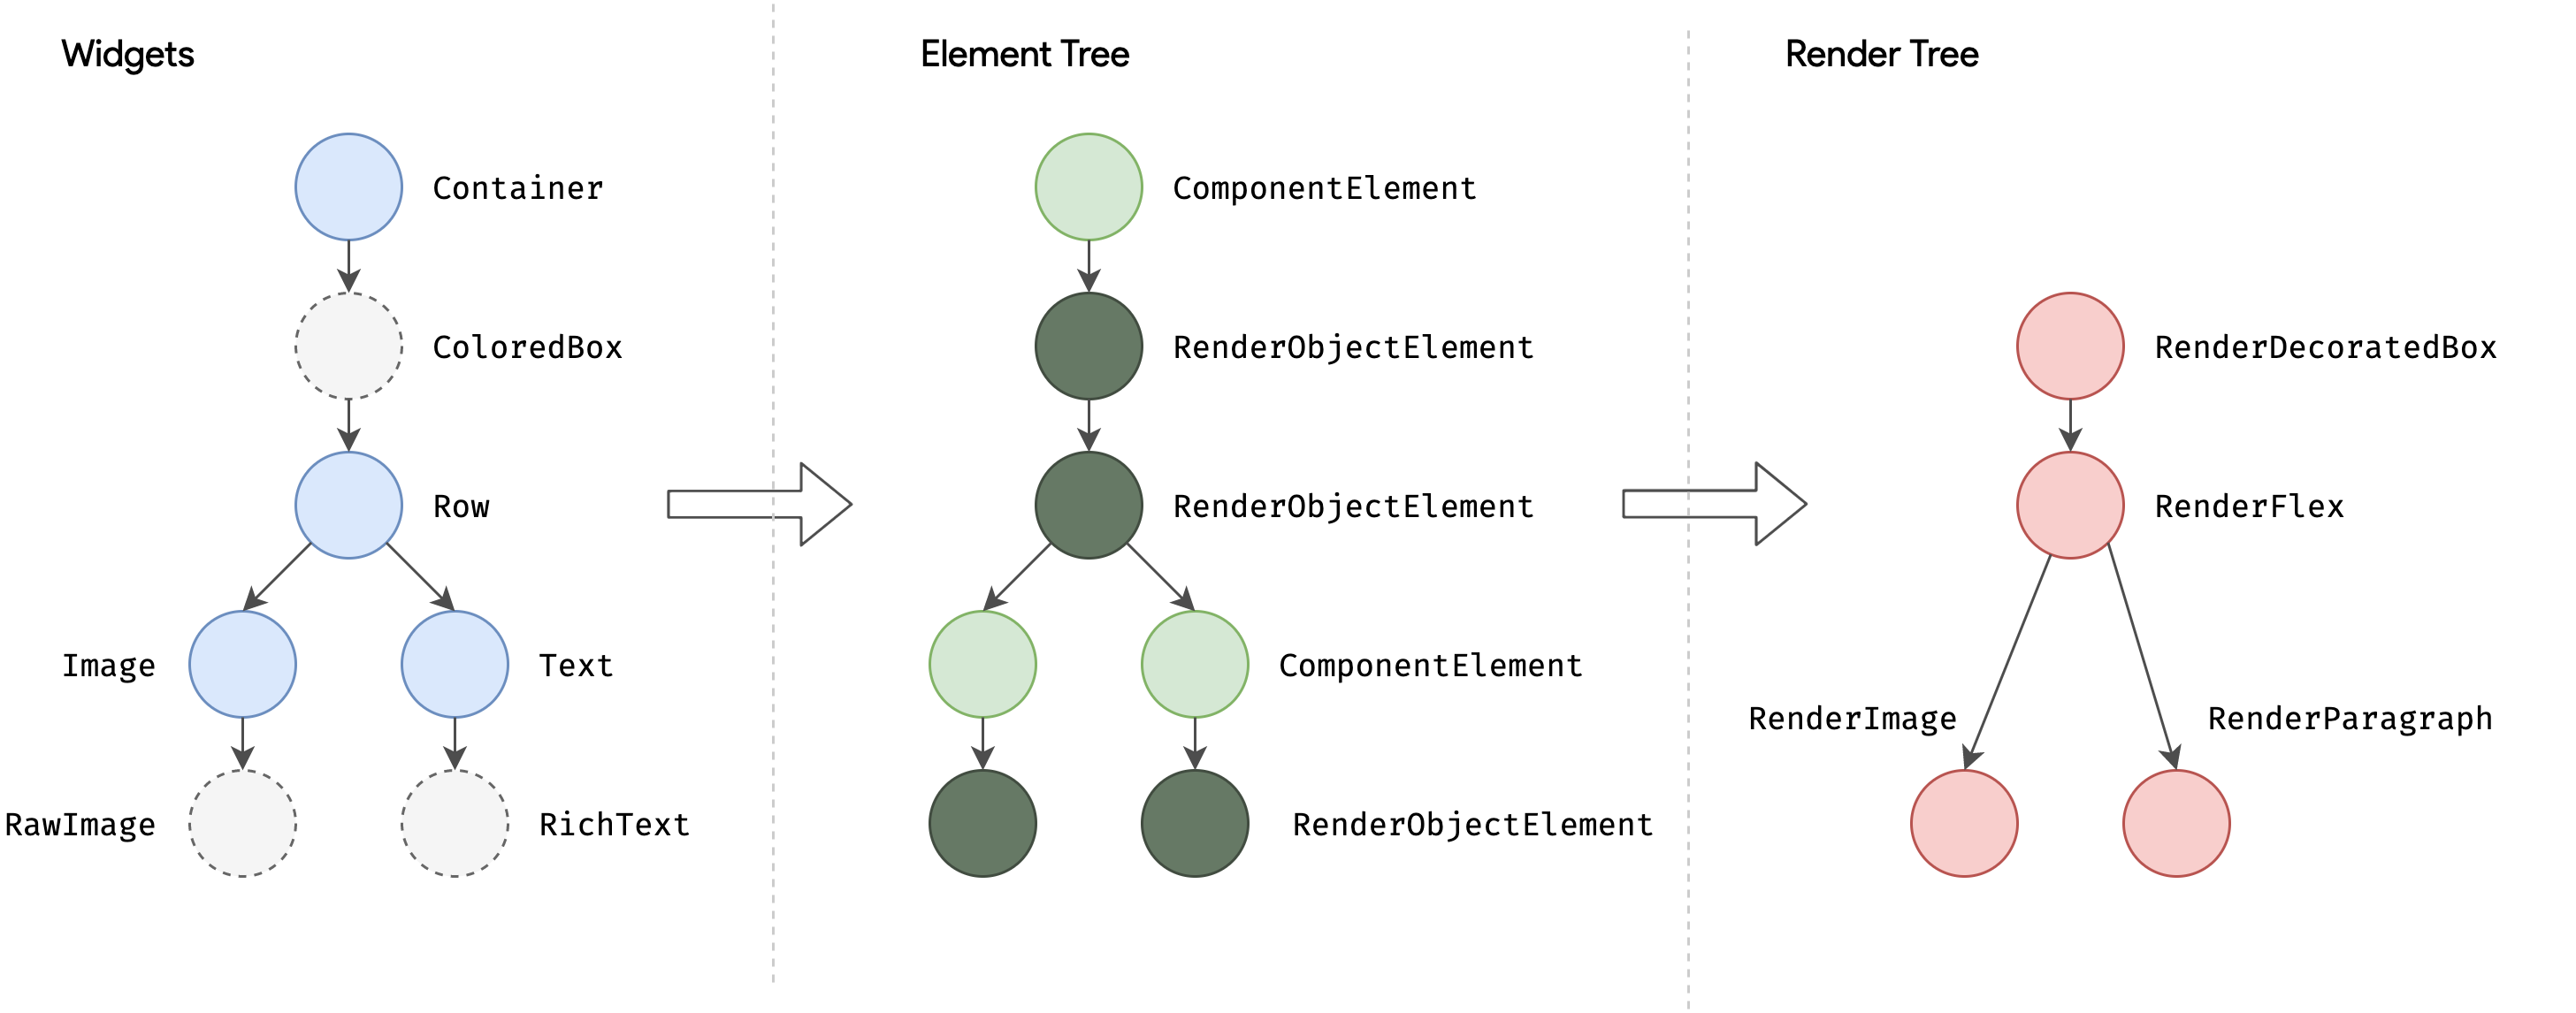
\includegraphics[width=\textwidth]{Flutter_trees}
    \caption[I tre alberi di Flutter]{Flutter usa tre alberi logici come rappresentazione delle proprie strutture: uno per i \textit{widget}, uno per gli \textit{element} e infine quello di \textit{render}.\footnotemark}
    \label{fig:flutter-trees}
\end{figure}
\footnotetext{Fonte: \url{https://docs.flutter.dev/resources/architectural-overview}}

L'albero di \textit{render} è una delle tre strutture logiche che Flutter usa per descrivere i propri oggetti e le proprie interfacce grafiche: il \textit{widget tree} rappresenta gli elementi di un \textit{widget} come uno \textit{stack} di \textit{widget}, messi in relazione con il loro elemento padre e i loro elementi figli. Nel caso del \textit{widget tree} rappresentato in figura \ref{fig:flutter-trees} esso rappresenta un \verb+Containter+ che contiene un \verb+ColoredBox+ che a sua volta contiene una \verb+Row+ e via dicendo. I \textit{widget} sono per definizione immutabili, quindi una modifica richiede necessariamente una distruzione e successiva ricreazione del \textit{widget} interessato.

\begin{lstlisting}[language=dart, caption={Codice rilevante per la parte grafica dell'\textit{app} di esempio di Flutter}]
    Widget build(BuildContext context) {
        return Scaffold(
          appBar: AppBar(
            title: Text(widget.title),
          ),
          body: Center(
            child: Column(
              mainAxisAlignment: MainAxisAlignment.center,
              children: <Widget>[
                const Text(
                  'You have pushed the button this many times:',
                ),
                Text(
                  '$_counter',
                  style: Theme.of(context).textTheme.headline4,
                ),
              ],
            ),
          ),
          floatingActionButton: FloatingActionButton(
            onPressed: _incrementCounter,
            tooltip: 'Increment',
            child: const Icon(Icons.add),
          ), // This trailing comma makes auto-formatting nicer for build methods.
        );
    }
\end{lstlisting}

Il codice precedente produce il seguente risultato (e il seguente \textit{widget tree}):

\begin{figure}[H]
    \centering
    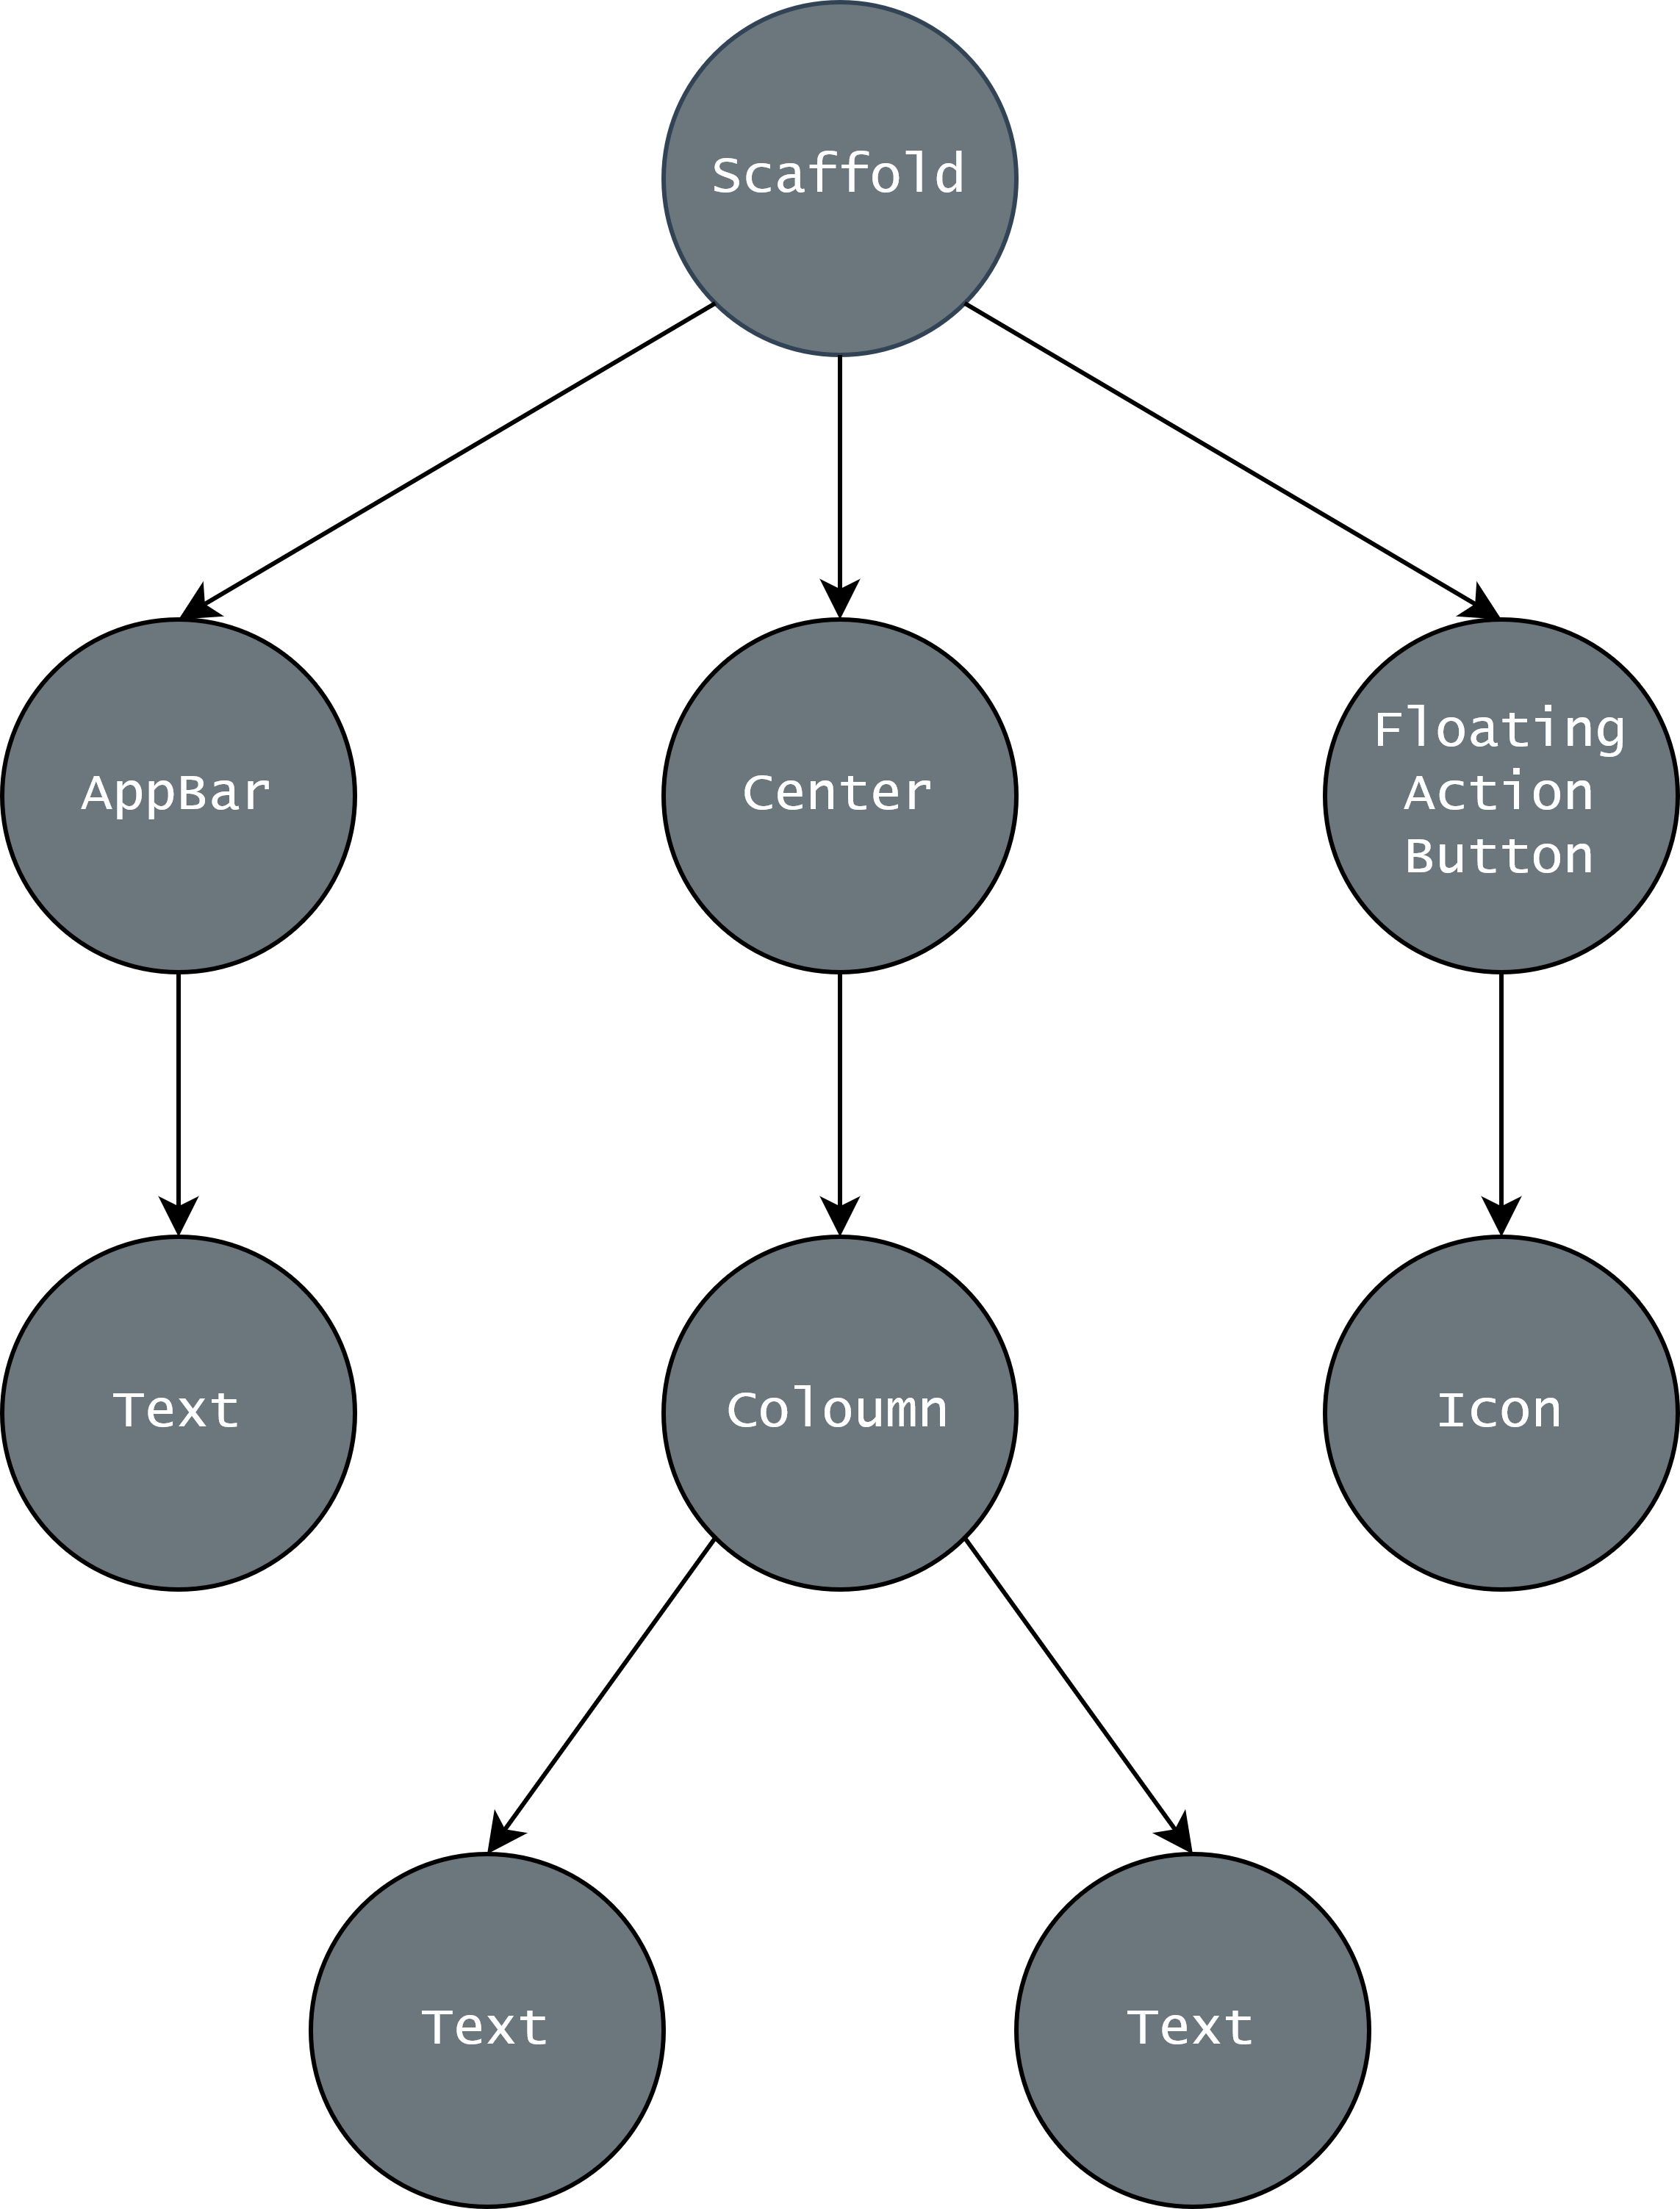
\includegraphics[height=8cm]{app_esempio_render_tree.png}\hspace{15mm}
    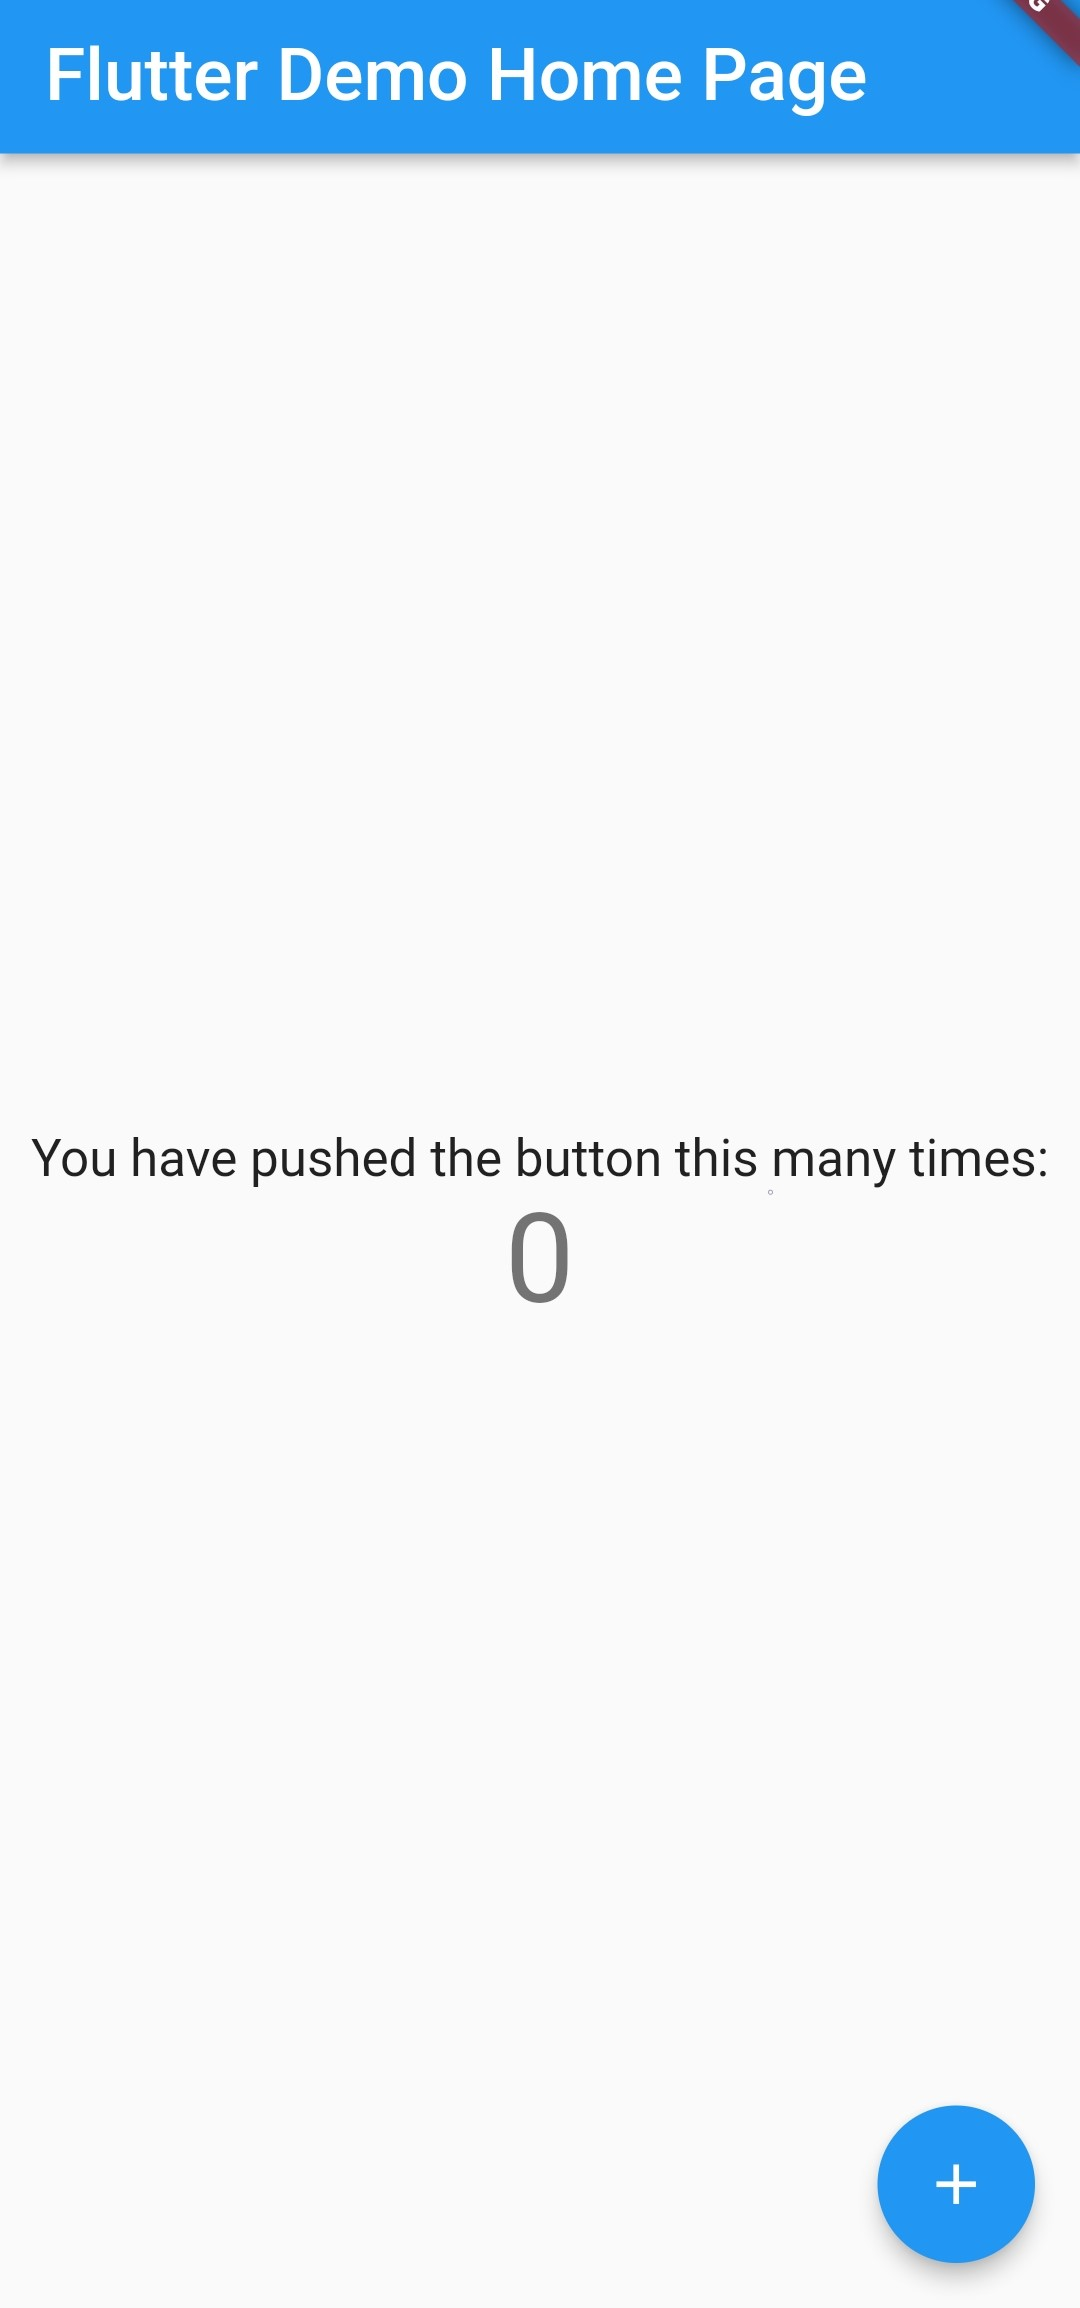
\includegraphics[height=8cm]{flutter_app_default.jpg}
    \caption[\textit{Widget tree} app esempio]{Il \textit{widget tree} dell'applicazione di esempio di Flutter e il suo risultato su Android}
\end{figure}

Per quanto riguarda le dimensioni delle varie componenti Flutter ragiona come segue: i padri passano ai figli (dall'altro verso il basso del \textit{widget tree}) dei \textit{"constraints"}, ovvero le dimensioni massime oltre le quali non possono cresce di dimensione, e i figli passano quindi ai padri (dal basso verso l'alto del \textit{widget tree}) le proprie dimensioni.\\
Il \textit{widget tree} è quello più importante da tenere a mente, e che più direttamente si interfaccia con il codice scritto dal programmatore. Torniamo però alla figura \ref{fig:flutter-trees} per parlare brevemente degli altri due alberi: l'\textit{element tree} rappresenta gli elementi che, a differenza dei \textit{widget}, sono mutabili e vengono definiti come "un'istanza di un \textit{Widget} in una particolare posizione dell'albero". Gli elementi sono responsabili di aggiornare l'interfaccia utente e fungono da ponte tra \verb+Widget+ e \verb+Render Object+.\\
Il \textit{render tree} rappresenta i \verb+Render Object+ e viene interpellato dal \textit{framework} per disegnare i componenti dell'interfaccia grafica. Una singola istanza di \verb+Render Object+ contiene tutte le informazioni riguardanti dimensioni, colori e logiche di \textit{layout} di un \verb+Widget+.\\
Abbiamo accennato che i \textit{widget} quando chiamano stato richiamano il proprio metodo \verb+build+ che provoca quindi una ricostruzione del \textit{widget} stesso. Questi \textit{widget} si chiamano \textit{"stateful}, e sono in diretta contrapposizone con quelli incapaci di modificarsi durante l'esecuzione, chiamati \textit{"stateless"}. 

\begin{lstlisting}[language=dart, label={lst:stateful_widget}, caption={Creazione \textit{stateless widget}}]
class MyApp extends StatelessWidget {
  //stateless widget che fa da radice per l'applicazione
  const MyApp({super.key});

  @override
  Widget build(BuildContext context) {
    return MaterialApp(
        home: const MyHomePage(title: 'Flutter Demo Home Page'),
    );
  }
}

class MyHomePage extends StatefulWidget {
  //qui passiamo allo stateful widget
  const MyHomePage({super.key, required this.title});
  final String title;

  @override
  //e qui creiamo lo stato vero e proprio
  State<MyHomePage> createState() => _MyHomePageState();
}


class _MyHomePageState extends State<MyHomePage> {
  int _counter = 0;

  void _incrementCounter() {
    //quando viene chiamata questa funzione viene
    //richiamato il metodo build, di fatto cambiando lo stato 
    //del widget e provocando un render dell'applicazione
    setState(() {
      _counter++;
    });
  }

  @override
  Widget build(BuildContext context) {}
}
\end{lstlisting}

Si nota immediatamente che l'uso degli \textit{stateful widget} provoca la scrittura di codice ridondante e si è quindi deciso di arginare questo problema, aumentando al contempo la condivisione di codice tra i \textit{widget}, introducendo i Flutter Hooks (ispirati dagli \textit{hooks} di React).
Vediamo quindi la riscrittura del codice mostrato in estratto \ref{lst:stateful_widget} opportunamente modificato usando un \verb+HookWidget+:

\begin{lstlisting}[language=dart, caption={Creazione \textit{hook widget}}]
class MyApp extends StatelessWidget {
  //stateless widget che fa da radice per l'applicazione
  const MyApp({super.key});

  @override
  Widget build(BuildContext context) {
    return MaterialApp(
        home: const MyHomePage(title: 'Flutter Demo Home Page'),
    );
  }
}

class MyHomePage extends HookWidget {
  //basta questa classe per fare tutti gli step
  //necessari al cambio di stato

  const MyHomePage({super.key, required this.title});
  final String title;

  Widget  build (BuildContext context){
    //_counter viene inizializzato a zero e reso
    //l'hook per il cambio di stato, quindi quando
    //il suo valore cambia viene provocato un rebuild
    final _counter = useState(0)

    return Scaffold(
      appBar: AppBar(),
      body: Center(),
      floatingActionButton: FloatingActionButton(
        //qui il valore di _counter cambia
        //provocando una rebuild
        onPressed: () => _counter.value++,
      )
    )
  }
}
\end{lstlisting}

\subsubsection{Method Channels}

\subsection{Realtà aumentata}
Uno dei punti centrali di questa tesi è la realtà aumentata e gli ancoraggi che è possibile posizionare all'interno di uno spazio tridimensionale, ed è quindi intelligente presentare preventivamente l'argomento e i concetti chiave.\\
La realtà aumentata consiste nel prendere lo spazio tridimensionale reale e trasporlo, tramite tecniche di mappatura, in formato digitale per poi poterci effettuare delle manipolazioni tramite \textit{software}. Ad esempio è possibile, nell'applicazione di Ikea, inquadrare il proprio salotto e posizionarci dei modelli poligonali\footnote{Detti anche \textit{asset} poligonali, prendono questo nome perché nel mondo della modellazione digitale tridimensionale le entità sono composte da triangoli adiacenti tra loro (poligoni appunto) che costruiscono una figura volumetrica. Questo perché il triangolo è la più semplice forma bidimensionale esistente, e quindi la meno esosa da calcolare.} della mobilia venduta dal colosso svedese.\\

\todo{} inserire pic ikea\\

Sebbene sia possibile immaginare lo spazio virtuale come un cubo vuoto all'interno del quale posizionare \textit{asset}, vengono applicate delle semplificazioni logiche per una questione di complessità ed efficienza di calcolo: lo spazio viene processato come una serie di piani bidimensionali sovrapposti a diverse altezze (una sorta di \textit{stack} di battaglie navali) e gli ancoraggi si legano quindi a una coppia di coordinate \textit{(x,y)} relativa al piano più la coordinata \textit{(z)} del piano stesso. Esistono inoltre piani orizzontali e verticali (non a caso alcune delle funzioni chiave di ARCore e ARKit servono a identificare gli spazi lisci).

\begin{figure}[H]
  \centering
  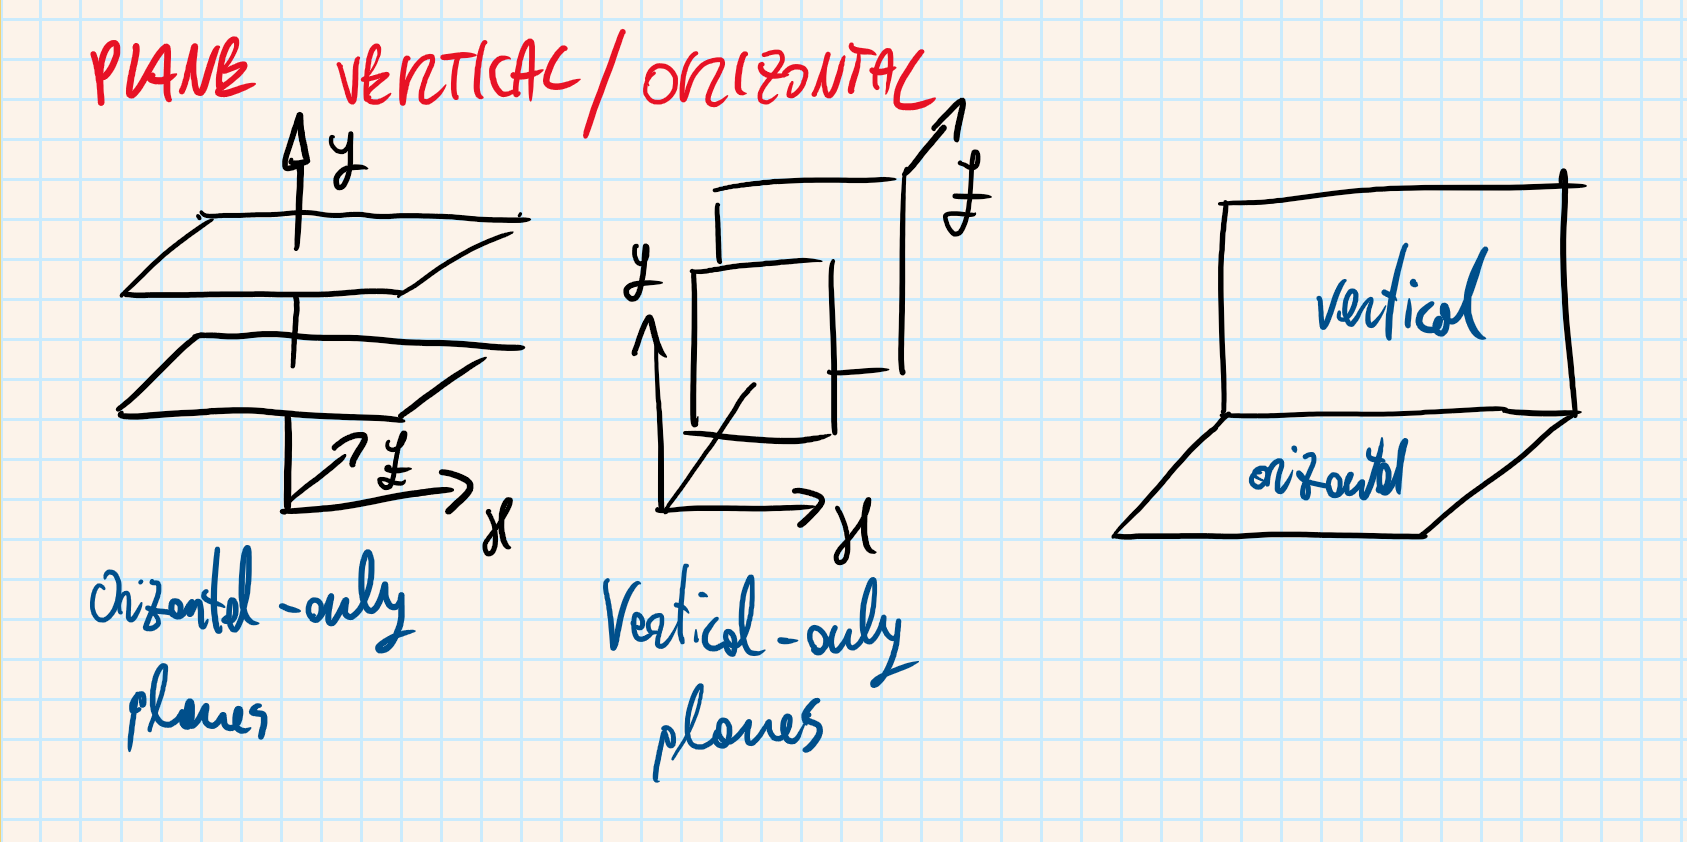
\includegraphics[width=\textwidth]{planes3D_temp}
  \caption[Piani in realtà aumentata]{caption \todo}
\end{figure}

Nella maggior parte dei casi è bene legare a un ancoraggio multiple entità diverse, questo perchè la \textit{pose} degli oggetti (ovvero rotazione verticale e orizzontale) è legata a quella della \textit{anchor} associata. Di conseguenza se vogliamo rappresentare in una stanza un insieme realistico di mobili (o meglio, di modelli poligonali e quindi gemelli digitali di mobili), se li leghiamo a un ancoraggio centrale rispetto alla stanza tutti gli elementi avranno sempre una posizione relativa corretta tra di loro. Se invece ogni elemento ha la sua \textit{anchor} potremmo vedere rotazioni errate oppure potrebbero spostarsi anche di qualche metro rispetto alla loro posizione originale.

\begin{figure}[H]
  \centering
  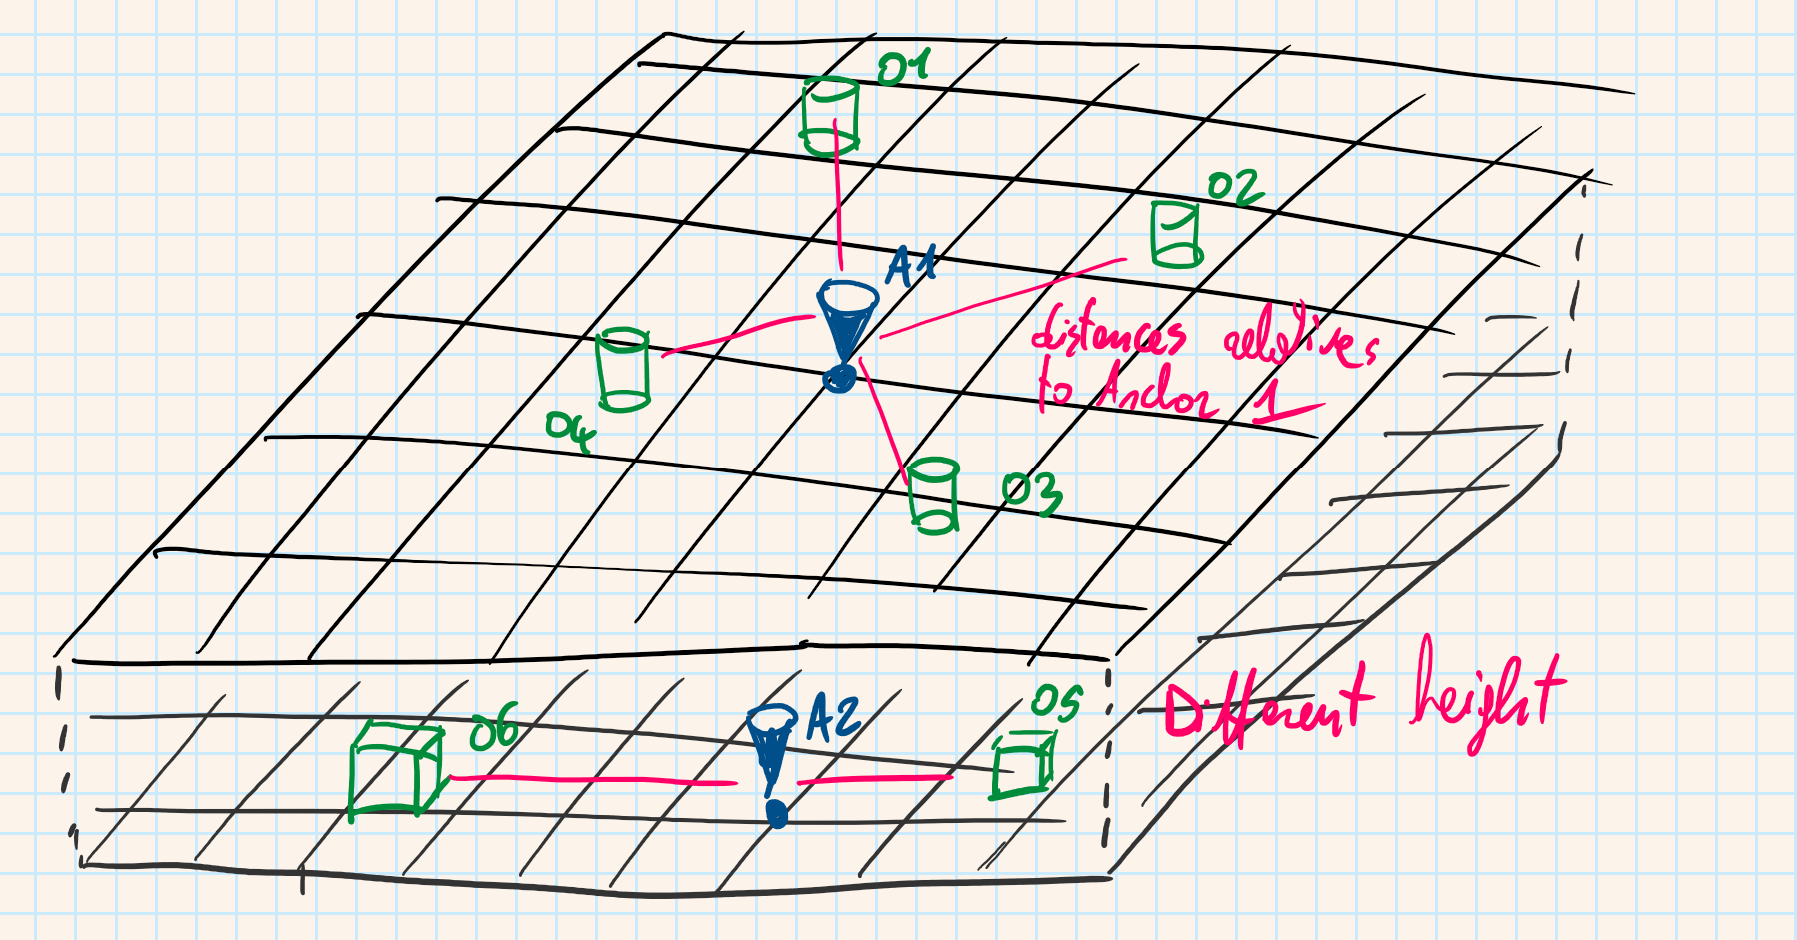
\includegraphics[width=\textwidth]{anchors_temp}
  \caption[Ancoraggi singoli per multipli elementi]{caption \todo}
\end{figure}

\subsection{Azure ToolKit}
Azure è l'ombrello sotto al quale vivono tutti i servizi \textit{cloud} di Microsoft esterni al pacchetto Office 365, e comprendono \textit{database} relazionali con scalabilità automatica (Azure SQL o Azure Cosmos DB), macchine virtuali remote (Virtual Machines e Azure Virtual Desktop) fino a funzionalità estremamente avanzate come Azure Kubernetes Service che fornisce un sistema automatizzato per rilasciare, scalare e gestire grandi applicativi \textit{sofware} (ad esempio per i \textit{data center}), oppure Azure Quantum che mette a disposizioni soluzioni per scrivere e far girare \textit{software} su \textit{hardware} quantistico.\\
Come si può notare la \textit{suite} Azure è indirizzata a utenti altamente specializzati e ancora più spesso a organizzazioni vere e proprie.

\begin{figure}[H]
  \centering
  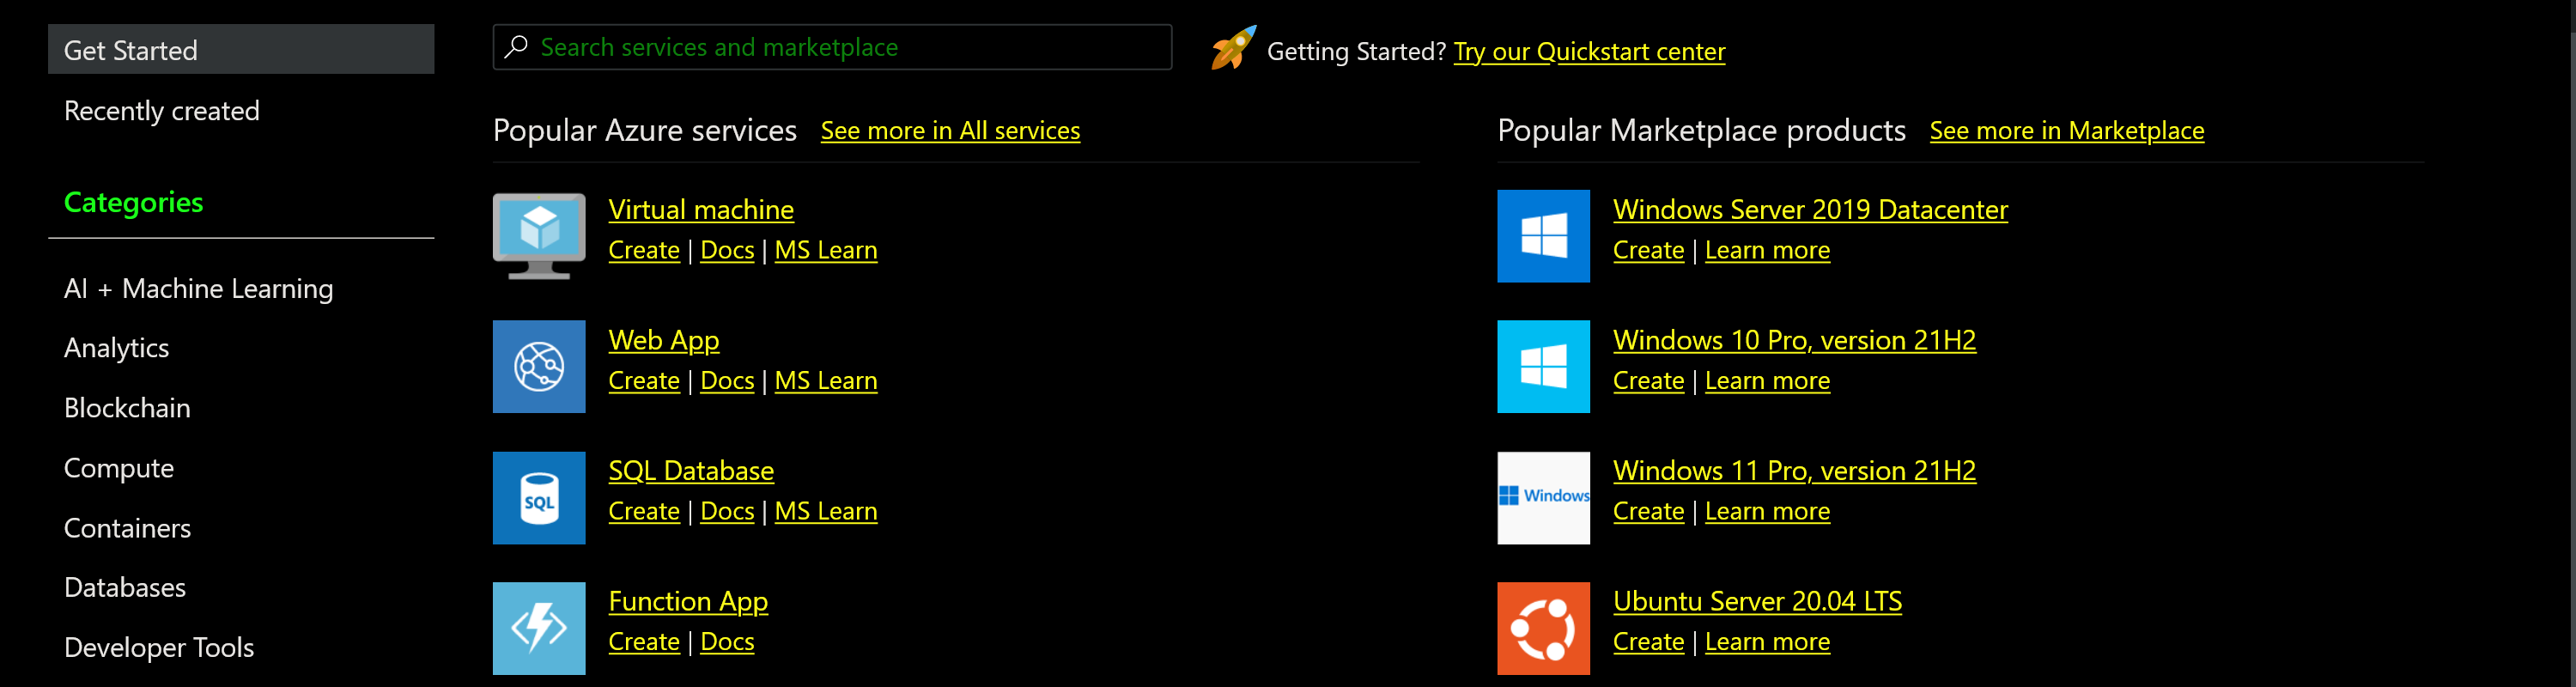
\includegraphics[width=\textwidth]{azure_resources}
  \caption[Azure Portal creazione risorse]{caption \todo}
\end{figure}

Per gli scopi di questo progetto ci serviremo di due degli strumenti forniti: l'Azure Portal e le \asa{}.\\
Il primo è semplicemente un portale online che serve a gestire, creare e monitorare tutte le risorse Azure legate a un \textit{account}, mentre le seconde sono il servizio di Microsoft per gestire ancoraggi geospaziali persistenti che possono anche essere utilizzati in un contesto di realtà aumentata.

\begin{figure}[H]
  \centering
  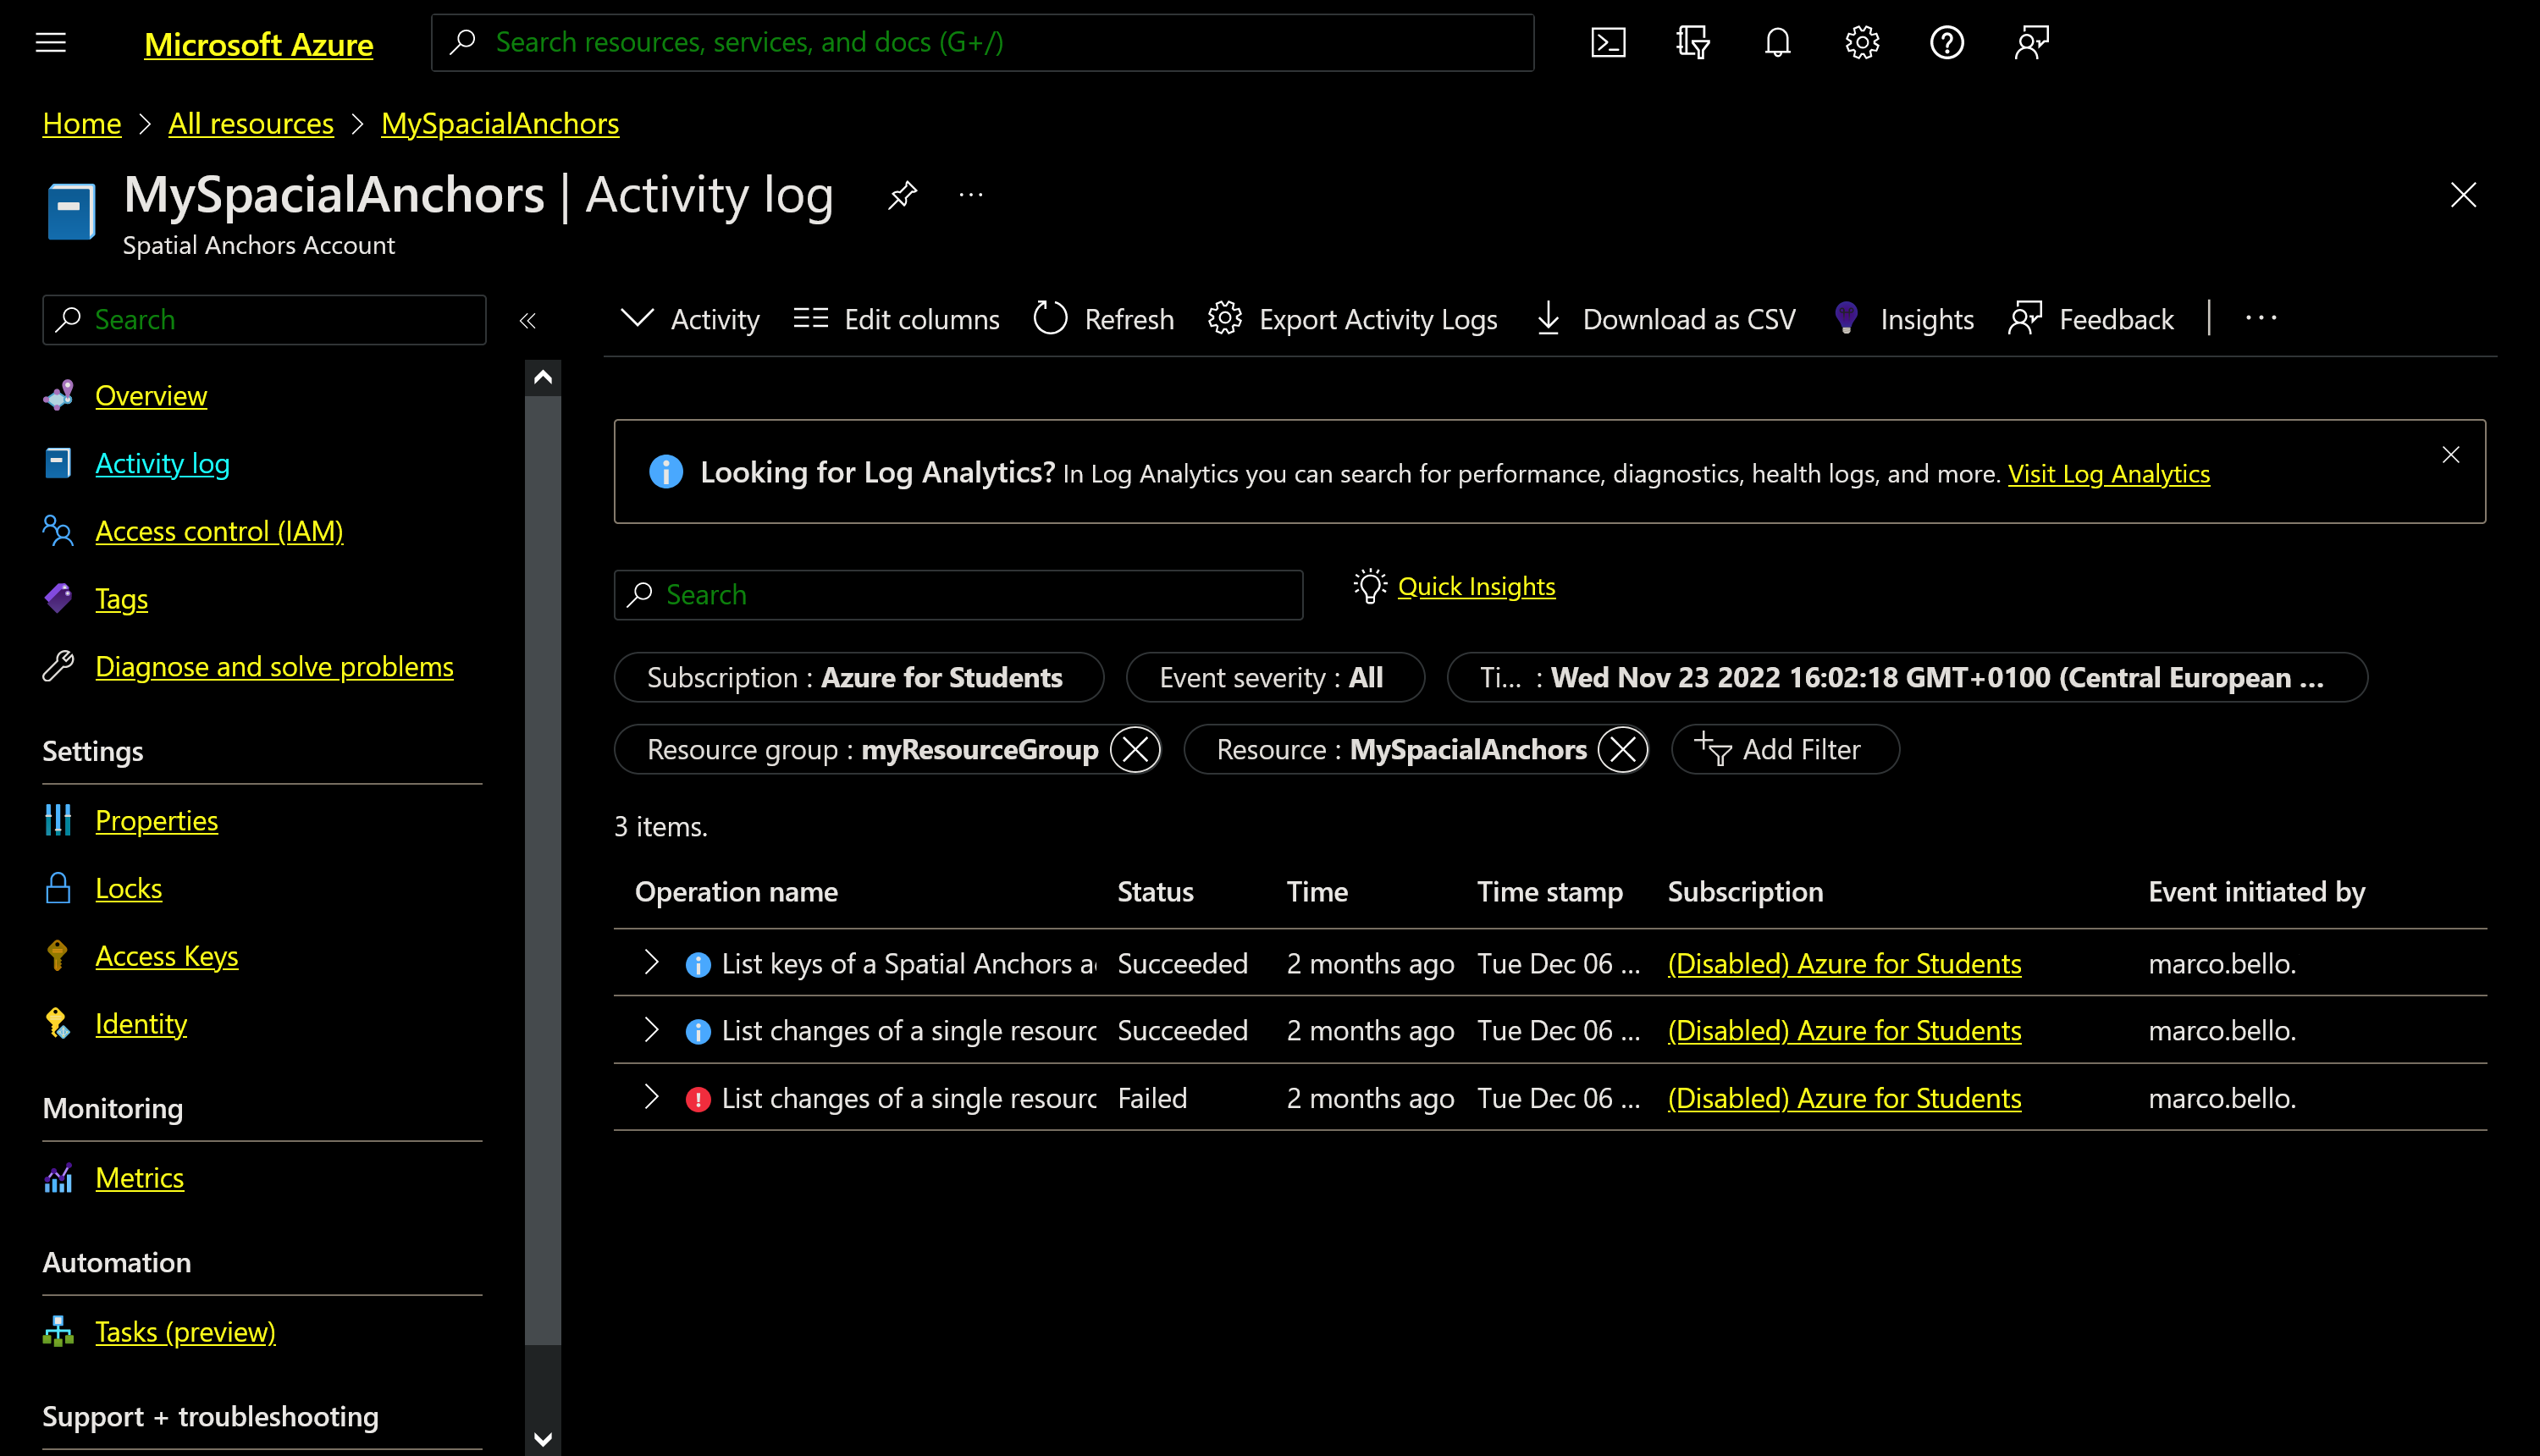
\includegraphics[width=\textwidth]{asa_azure_portal}
  \caption[Azure Portal]{caption \todo}
\end{figure}

Le \asa{} forniscono tre \sdk{}s, uno per Microsoft HoloLens, uno per iOS appoggiandosi su ARKit e uno per Android basato su ARCore, possono collegarsi tra loro creando relazioni che formano dei veri e propri percorsi (funzionalità usata spesso nel contesto degli \textit{asset} aziendali, ad esempio in una stessa linea produttiva) e possono essere contenuti dentro un \textit{resource group} di Azure che funge da contenitore di risorse dentro al quale esse vengono create e gestite.

\subsection{Framework realtà aumentata per Flutter}
Essendo lo scopo di questo stage, e quindi il caso di studio di questa tesi, l'implementazione di una vista in realtà aumentata (nello specifico sfruttando \asa{}) in un'applicazione preesistente sviluppata in Flutter, una grossa parte del lavoro svolto si è incentrato sullo studio dei \textit{framework} e/o \textit{plug-in} disponibili.\\
Sfortunatamente, complici la giovinezza di Flutter e la scarsa diffusione di tecnologie per la realtà aumentata, le opzioni disponibili sono alquanto ridotte:
\begin{itemize}
    \item \aplug{}: \textit{plugin}\footnote{Fonte: \url{https://pub.dev/packages/ar_flutter_plugin}} che punta a implementare le componenti in realtà aumentata in modalità \textit{cross-platform}, quindi adattandosi autonomamente ad Android e iOS (sfruttando tuttavia le Cloud Anchor di Google). Nasce partendo da due plugin più specializzati: 
    \begin{itemize}
        \item arcore\_flutter\_plugin per Android\footnote{Fonte: \url{https://github.com/giandifra/arcore_flutter_plugin}};
        \item arkit\_flutter\_plugin per iOS\footnote{Fonte: \url{https://github.com/olexale/arkit_flutter_plugin}};
    \end{itemize}
    \item ARwayKit: \textit{framework} che mira a fornire un'integrazione semplificata, e in parte già completata, di una componente in realtà aumentata (ottenuta tramite \asa{}) in Flutter tramite vista in Unity.
\end{itemize}
E' necessario notificare che al momento della stesura di questo testo non è più possibile accedere liberamente alla documentazione relativa ad ARwayKit\footnote{Fonte: \url{https://app.gitbook.com/s/-MCtct_TY9f3e8PrcV9T/arwaykit-with-flutter/quickstart-in-flutter}}, tuttavia è ancora reperibile un articolo sul sito Medium che ricalca la guida introduttiva precedentemente fornita dal sito ufficiale dell'azienda\footnote{Fonte: \url{https://medium.com/arway/building-ar-navigation-apps-with-flutter-and-arwaykit-280b69401cd9}}. 
E' anche possibile trovarne una versione nella Wayback Machine\footnote{Fonte: \url{https://web.archive.org/web/20220525060655/https://docs.arway.app/arwaykit-with-flutter/quickstart-in-flutter}}.

\subsubsection{ARWayKit}
ARwayKit è un \textit{framework} formato da un insieme di componenti che si pone l'obiettivo di fornire un'esperienza in realtà aumentata persistente, e lo persegue fornendo una \sdk{} Unity, un'applicazione di mappatura e un insieme di \api{}s REST\footnote{Conosciute anche come RESTful API, sono delle \api{}s che si conformano allo stile architetturare e alle norme per sistemi distributi chiamato \textit{representational state transfer} largamente utilizzato nella comunicazione \textit{web}.}, che implementa le componenti in realtà aumentata in Flutter sfruttando il \textit{plugin} flutter\_unity\_widget\footnote{Fonte: \url{https://pub.dev/packages/flutter_unity_widget}}.\\
E' multipiattaforma, implementa gli ancoraggi tramite \asa{} e funziona in ambienti \textit{"GPS-denied"}, ovvero dove i dati di posizione del \textit{global positioning system}\footnote{Sistema di satelliti in grado di fornire a un ricevitore le sue coordinate geografiche.} non vengono utilizzati per muoversi all'interno dell'ambiente virtuale (oppure ambienti con protocolli di \textit{privacy} elevati), il che lo rende apparentemente perfetto per il caso d'uso specifico di questa tesi. 

\begin{figure}[H]
  \centering
  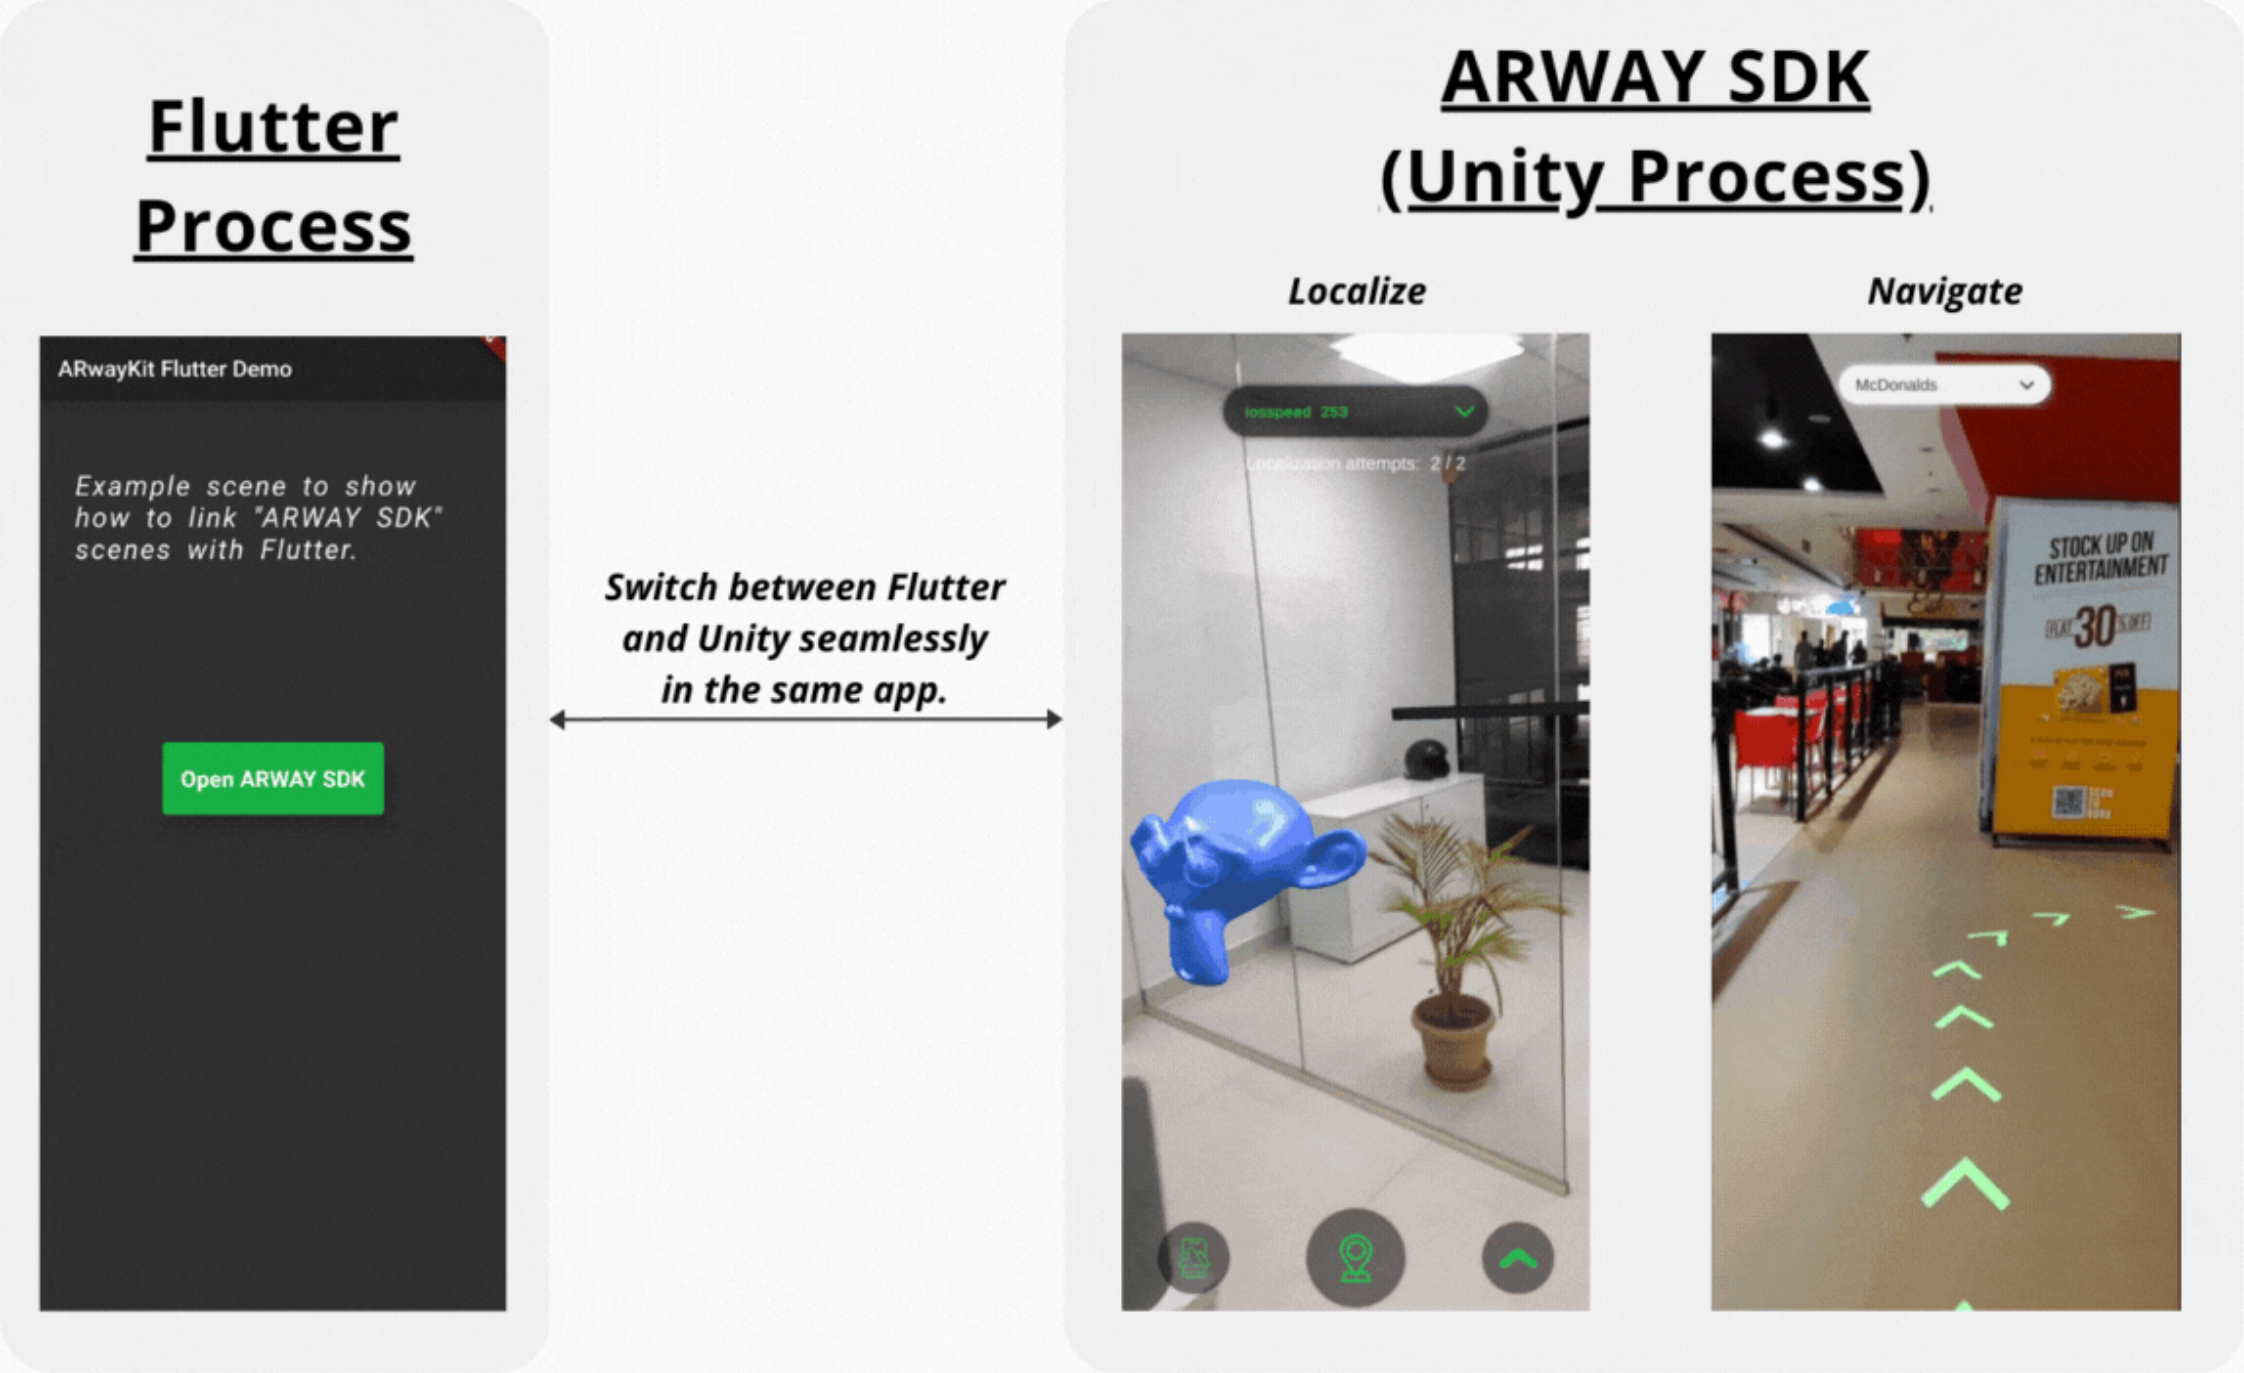
\includegraphics[width=\textwidth]{ARwayKit_samplegif_screenshot}
  \caption[Realtà aumentata con ARwayKit]{Immagine esempio di utilizzo realtà aumentata con ARwayKit\footnotemark}
\end{figure}
\footnotetext{Fonte: \url{https://medium.com/arway/building-ar-navigation-apps-with-flutter-and-arwaykit-280b69401cd9}}

Tuttavia, presenta delle criticità: in primo luogo obbliga l'uso di Unity (sfruttando la sua caratteristica peculiare di poter essere importato come fosse una libreria) per sviluppare la vista in realtà aumentata, il che comporta non solo dover imparare il linguaggio ma dover anche configurare ulteriori componenti (come ad esempio Unity Hub) che poi devono essere adottati assieme a quelli già in uso, appesantendo quindi il processo di codifica.\\
In secondo luogo troviamo invece il problema maggiore: la vista verrebbe realizzata nativamente in Unity, ovvero si tratta di una componente Unity separata rispetto all'applicazione che la lancia.
Questo renderebbe complesso se non impossibile usare dentro essa delle funzionalità Flutter: ad esempio, un bottone a schermo sarebbe un pulsante Unity, non Flutter, obbligando quindi poi a costruire una mappatura tra i due linguaggi per ogni funzionalità visualizzata.\\ 
Una vista così costruita non solo è scomoda da programmare, ma anche difficile da manutenere.

\subsubsection{ar\_flutter\_plugin}
\aplug{} è un \textit{plugin open-source} collaborativo estremamente giovane (il primo \textit{commit} sulla \textit{repository} pubblica risale al 6 febbraio 2021\footnote{Fonte: \url{https://github.com/CariusLars/ar_flutter_plugin/commit/da9ab148219d833755ef7a9b1e3536a3cae865d1}}) che si pone l'obiettivo di implementare componenti in realtà aumentata in Flutter.\\
Per raggiungere lo scopo si serve della libreria archiviata Sceneform\footnote{Fonte: \url{https://developers.google.com/sceneform/develop}}, che si occupa di "renderizzare scene tridimensionali realistiche in applicazioni in realtà aumentata o meno, senza dover imparare OpenGL".\\
L'architettura di \aplug{} è composta da due componenti: una \api{} multipiattaforma unificata che fornisce un'interfaccia alle applicazioni tramite il \textit{plugin} e le implementazioni specifiche per le piattaforme Android (in Kotlin) e iOS (in Swift) costruite su ARCore e ARKit rispettivamente, così da garantire accesso continuativo nel tempo a funzionalità aggiornate.\\
\aplug{} espone dei \textit{widget} che possono essere inclusi nel \textit{widget tree} (fig. \ref{fig:flutter-trees}) dell'applicazione cliente e delle classi \textit{manager} per gestire funzionalità e logiche di controllo del \textit{plugin} e delle componenti in realtà aumentata: il \textit{session manager} gestisce le configurazioni di tracciamento (ad esempio se gestire piani orizzontali, verticali o entrambi), opzioni di \textit{debugging} (come la visualizzazione dei piani) e le \textit{callbacks} per gli \textit{hit-test}\footnote{Immaginando un vettore che parte dall'ottica del dispositivo e tocca una superficie, possiamo considerare quel contatto un \textit{"hit"}. Con \textit{hit-testing} si intende valutare la capacità di tracciare correttamente lo spazio inteso come distanza tra i punti dello stesso e il dispositivo.} e i \textit{gesture events}\footnote{Azioni che il sistema deve fare quando vengono effettuati degli \textit{input} tramite \textit{touch screen} del dispositivo}.\\
L'\textit{object manager} gestisce i nodi in realtà aumentata del \textit{plugin} che servono ad astrarre rispetto alle funzionalità native delle varie piattaforme (ARCore e ARKit ad esempio) e permettono di aggiungere, modificare o rimuovere nodi basandosi su formati GLTF2 o GLB che possono essere caricati a \textit{runtime} da un \textit{file system} o dalla rete.\\
L'\textit{anchor manager} contiene funzioni per caricare e ottenere ancoraggi da servizi \textit{cloud} servendosi della \api{} Google Coud Anchor. Gli ambienti virtuali registrati localmente possono essere salvati in rete e comparati con quelli già in \textit{storage} persistente per scaricare ancoraggi e oggetti precedentemente posizionati nella scena.\\
Infine il \textit{location manager} si occupa di fornire le coordinate del \textit{global positioning system}  per permettere un'interrogazione efficiente degli ancoraggi basati su posizione geografica.\\
Il \textit{plugin} ha un'architettura largamente \textit{clout-agnostic}, ovvero che non si interessa dell'implementazione specifica per i servizi di salvataggio persistente, il che gli permette di usare facilmente gestori di contenuti esterni.

\subsubsection{Confronto}
Vediamo quindi di schematizzare e mettere a confronto pregi e difetti delle due soluzioni trovate.\aCapo{}

\textbf{Pregi ARwayKit:}
\begin{itemize}
  \item Implementa nativamente le \asa{};
  \item Funziona in ambienti \textit{GPS-denied};
  \item E' pensato per uso aziendale.
\end{itemize}

\textbf{Difetti ARwayKit:}
\begin{itemize}
  \item La vista e le componenti in realtà aumentata non sono implementate in Flutter;
  \item Richiede l'uso di Unity che, essendo un motore per videogiochi, ha funzionalità in più (e in meno) non necessarie (e necessarie) rispetto a un uso aziendale;
  \item Ha una documentazione difficile da reperire e di dubbia completezza;
  \item E' codice propietario, quindi non c'è modo di visionare il sorgente.
\end{itemize}

\textbf{Pregi \aplug{}:}
\begin{itemize}
  \item La vista e le componenti in realtà aumentata sono implementate in Flutter;
  \item Ha un documentazione discreta;
  \item E' \textit{open-source}, quindi al bisogno è possibile visionare il codice sorgente;
  \item E' pensato per uso aziendale;
  \item La struttura logica, divisa nei vari \textit{manager}, è modulare e chiara da comprendere, il che dovrebbe facilitarne modifica ed estensione;
  \item Promette di essere \textit{cloud-agnostic}, quindi favorisce l'uso di gestorie sterni come ad esempio \asa{} 
\end{itemize}

\textbf{Difetti \aplug{}:}
\begin{itemize}
  \item Non implementa nativamente le \asa{}, usando invece le Google Cloud Anchors;
  \item Non è chiaro se funzioni nativamente in ambienti \textit{GPS-denied};
\end{itemize}

\textbf{Confronto schematico:}

{
  \setlength{\freewidth}{\dimexpr\textwidth-10\tabcolsep}
  \renewcommand{\arraystretch}{1.5}
  \centering
  \setlength{\aboverulesep}{0pt}
  \setlength{\belowrulesep}{0pt}
  \begin{longtable}{C{.6\freewidth} C{.2\freewidth} C{.2\freewidth}} 
     \toprule 
  \cellcolor{red}\textcolor{white}{\textbf{Caratteristica}} &
  \cellcolor{red}\textcolor{white}{\textbf{ARwayKit}} &
  \cellcolor{red}\textcolor{white}{\textbf{Plugin}}\\
  \midrule
  \endhead
  
  \cellcolor{black!20}\asa{} native & \cellcolor{green!20}SI & \cellcolor{red!20}NO\\
  \cellcolor{black!20}Ambienti \textit{GPS-denied} & \cellcolor{green!20}SI & \cellcolor{orange!20}NON CHIARO\\
  \cellcolor{black!20}Vista realtà aumentata implementata in Flutter & \cellcolor{red!20}NO & \cellcolor{green!20}SI\\
  \cellcolor{black!20}Codice sorgente visibile & \cellcolor{red!20}NO & \cellcolor{green!20}SI\\
  \cellcolor{black!20}Pensato per uso aziendale & \cellcolor{green!20}SI & \cellcolor{green!20}SI\\

  \bottomrule
  \rowcolor{white} 
  \caption{Confronto \textit{framework} per realtà aumentata}
  \end{longtable}
}

E' stato infine scelto \aplug{} rispetto ad ARwayKit per evitare di interfacciarsi con Unity e per la necessità di avere la vista in realtà aumentata implementata direttamente in Flutter.

\section{Analisi dei requisiti}
Di seguito sono riportati i requisti individuati nel piano di lavoro proposto e a seguito di opportuni confronti con il tutor aziendale. Essi sono catalogati secondo la dicitura:
\begin{center}
    \textbf{R[Obbligatorietà][Tipologia][Codice]}
\end{center}
dove:
\begin{itemize}
    \item \textbf{Obbligatorietà}: specifica quanto un requisito sia vincolante per la riuscita del prodotto e può assumere i seguenti valori:
    \begin{itemize}
        \item \textbf{1: } Requisito obbligatorio;
        \item \textbf{2: } Requisito desiderabile ma non essenziale per il funzionamento;
        \item \textbf{3: } Requisito opzionale.
    \end{itemize}
    \item \textbf{Tipologia}: specifica la tipologia del requisito e può assumere i seguenti valori:
    \begin{itemize}
        \item \textbf{F: }\textit{funzionale,} determina una funzionalità necessaria all'applicazione;
        \item \textbf{V: }\textit{vincolo,} riguarda una caratteristica del prodotto decisa a monte.
    \end{itemize}
    \item \textbf{Codice}: identifica univocamente un requisito all'interno della sua tipologia (ovvero possono esistere due requisiti con lo stesso codice a patto che siano uno funzionale e uno di vincolo). Per i requisti subordinati si usa il "punto" come divisorio (\textit{ReqPadre, ReqPadre.Figlio1})
\end{itemize}

\subsection{Requisiti funzionali}
{
    \setlength{\freewidth}{\dimexpr\textwidth-10\tabcolsep}
    \renewcommand{\arraystretch}{1.5}
    \centering
    \setlength{\aboverulesep}{0pt}
    \setlength{\belowrulesep}{0pt}
    \rowcolors{2}{red!10}{white}
    \begin{longtable}{C{.15\freewidth} | C{1\freewidth}}
       \toprule
    \rowcolor{red}
    \textcolor{white}{\textbf{Codice}}&
    \textcolor{white}{\textbf{Descrizione}}\\
    \toprule
    \endhead

    R1F1 & Il \textit{plugin} deve rappresentare \textit{asset} tramite ancoraggio in realtà aumentata\\
    R1F2 & Il \textit{plugin} deve rappresentare \textit{ticket} tramite ancoraggio in realtà aumentata\\
    R1F3 & Il \textit{plugin} deve integrare gli ancoraggi tramite \asa{}\\
    R1F3.1 & Permettere aggiunta di \asa\\%C
    R1F3.2 & Permettere recupero e visualizzazione di \asa\\%R
    R2F3.3 & Permettere modifica di \asa\\%U
    R1F3.4 & Permettere eliminazione di \asa\\%D
    %API BACKEND
    R1F4 & Comunicare con le \api{}s di Syn\\
    R1F4.1 & Ricevere \textit{asset} con ancoraggio associato\\
    R1F4.2 & Aggiungere \textit{asset} con ancoraggio associato\\
    R2F4.3 & Ricevere \textit{ticket} con ancoraggio associato\\
    R2F4.4 & Aggiungere \textit{ticket} con ancoraggio associato\\
    %UI FLUTTER
    R1F5 & Utente deve poter vedere quali \textit{asset} hanno ancoraggio associato\\
    R2F6 & Utente deve poter vedere quali \textit{ticket} hanno ancoraggio associato\\
    R1F7 & Utente deve poter raggiungere l'ancoraggio in vista in realtà aumentata dalla schermata dell'\textit{asset}\\
    R1F8 & \textit{On-Tap} su una ancoraggio deve aprire una \textit{bottom sheet} contestuale\\
    R1F8.1 & \textit{Bottom sheet} deve presentare identificatore per \textit{asset} o \textit{ticket} associato alla ancoraggio\\
    R1F8.2 & \textit{Bottom sheet} associato a un \textit{asset} mostra ultimi tre \textit{ticket} aperti\\
    R1F8.3 & \textit{Bottom sheet} deve fornire \textit{Call-To-Action} per eliminare l'ancoraggio\\
    R1F8.4 & \textit{Bottom sheet} deve fornire \textit{Call-To-Action} per raggiungere pagina di dettaglio\\
    R1F9 & Le informazioni contestuali di un \textit{ticket} includono data e ora di creazione\\
    %UI AR
    R1F10 & Gli ancoraggi hanno rappresentazione visiva contestuale\\ 
    R1F11 & \textit{On-Tap} sullo spazio permette di creare una ancoraggio in posizione\\
    R1F11.1 & Ancoraggio posizionato nello spazio può essere salvato\\
    R1F11.2 & Ancoraggio posizionato nello spazio può essere eliminato\\
    R1F12 & Il salvataggio di un'ancoraggio è disponibile solo quando è sicuro vada a buon fine\\
    R1F12.1 & Viene mostrato a schermo un feedback riguardo il livello di sicurezza raggiunto\\
    \bottomrule
    \rowcolor{white} 
    \caption{Tabella dei requisiti funzionali}
    \label{tab:requisiti-funzionali}
    \end{longtable}
}

\subsection{Requisiti di vincolo}
{
    \setlength{\freewidth}{\dimexpr\textwidth-10\tabcolsep}
    \renewcommand{\arraystretch}{1.5}
    \centering
    \setlength{\aboverulesep}{0pt}
    \setlength{\belowrulesep}{0pt}
    \rowcolors{2}{red!10}{white}
    \begin{longtable}{C{.15\freewidth} C{1\freewidth}} 
       \toprule
    \rowcolor{red}
    \textcolor{white}{\textbf{Codice}}&
    \textcolor{white}{\textbf{Descrizione}}\\
    \toprule
    \endhead

    R1V1 & \textit{Framework} scelto funziona su Android\\
    R2V2 & \textit{Framework} scelto funziona su iOS\\
    R1V3 & \textit{Framework} scelto si integra con le \api{}s di Syn\\
    R1V3.1 & \textit{Framework} ottiene con ancoraggio associato i dati degli \textit{asset}\\
    R1V3.2 & \textit{Framework} ottiene con ancoraggio associato i dati dei \textit{ticket}\\
    R1V4 & Il \textit{framework} scelto utilizza asa\\
    R1V5 & La vista in realtà aumentata deve essere sviluppata in Flutter\\
    \bottomrule
    \rowcolor{white} 
    \caption{Tabella dei requisiti di vincolo}
    \label{tab:requisiti-di-vincolo}
    \end{longtable}
}

\subsection{Riepilogo requisiti}
Sono stati individuati un totale di 36 requisiti, 29 funzionali e 7 di vincolo, di seguito schematizzati:
{
    \setlength{\freewidth}{\dimexpr\textwidth-10\tabcolsep}
    \renewcommand{\arraystretch}{1.5}
    \centering
    \setlength{\aboverulesep}{0pt}
    \setlength{\belowrulesep}{0pt}
    \rowcolors{2}{red!10}{white}
    \begin{longtable}{C{.25\freewidth} C{.2\freewidth}} 
       \toprule
    \rowcolor{red}
    \textcolor{white}{\textbf{Obbligatorietà}}&
    \textcolor{white}{\textbf{Quantità}}\\
    \toprule
    \endhead

    Obbligatori & 31\\
    Desiderabili & 5\\
    \bottomrule
    \rowcolor{white} 
    \caption{Numero di requisiti per obbligatorietà}
    \label{tab:requisiti-obbligatorieta}
    \end{longtable}
}

{
    \setlength{\freewidth}{\dimexpr\textwidth-10\tabcolsep}
    \renewcommand{\arraystretch}{1.5}
    \centering
    \setlength{\aboverulesep}{0pt}
    \setlength{\belowrulesep}{0pt}
    \rowcolors{2}{red!10}{white}
    \begin{longtable}{C{.25\freewidth} C{.2\freewidth}} 
       \toprule
    \rowcolor{red}
    \textcolor{white}{\textbf{Tipologia}}&
    \textcolor{white}{\textbf{Quantità}}\\
    \toprule
    \endhead

    Funzionali & 29\\
    Di Vincolo & 7\\
    \bottomrule
    \rowcolor{white} 
    \caption{Numero di requisiti per tipologia}
    \label{tab:requisiti-tipolgia}
    \end{longtable}
}


%************************************************************************************************************

\section{Pianificazione}
La natura estremamente sperimentale di questo progetto ha reso vano ogni tentativo di pianificare accuratamente il lavoro (complici anche le problematiche che vedremo nella sezione \ref{sec:difficolta_incontrate}).\\
Per questo motivo, una volta scelto il \textit{framework} per l'implementazione di \asa{} in Flutter l'approccio scelto è stato di \textit{trial-and-error}, e ha impegnato una buona parte del tempo di stage sia mio che dei membri di Datasoil responsabili del \textit{frontend}.\\
E' stata comunque fatta, di settimana in settimana, una scaletta degli obiettivi da raggiungere per il lunedì successivo, tuttavia si è riusciti a seguirla solo fintanto che comprendeva lo studio delle tecnologie e la creazione di brevi \textit{proof of concept} (ad esempio costruire un'applicazione in Dart e poi tradurre i suoi \textit{stateful widget} in \textit{hook widget}).\\
Riporto quindi la programmazione settimanale che, siccome questo documento è scritto al termine dei lavori, è in parte anche un rendicontazione:

\begin{itemize}
  \item \textbf{Settimana 1:} 
      \begin{itemize}
          \item Installazione e configurazione del \textit{framework} Flutter e della \sdk{} per Android 
          \item Configurazione emulatore Android (scelto Pixel 6 API 33) e 
          \textit{developers options} sul mio telefono personale;
          \item Configurazione \vsc{} e \astudio;
          \item Sviluppo di applicazione d'esempio con Flutter che sfrutta gli \textit{stateful widgets};
      \end{itemize} 
  \item \textbf{Settimana 2:} 
      \begin{itemize}
          \item Studio degli \textit{hook widgets};
          \item Traduzione degli \textit{stateful widgets} dell'applicazione d'esempio in \textit{hook widgets};
          \item Sviluppo applicazione d'esempio con gli \textit{hook widgets};
      \end{itemize}
  \item \textbf{Settimana 3:} 
      \begin{itemize}
          \item Studio delle \asa;
          \item Creazione risorse necessarie nel portale di Azure;
          \item Sviluppo applicazione di esempio per \asa{};
      \end{itemize}
  \item \textbf{Settimana 4:} Studio dei metodi per implementare le asa in Flutter:
      \begin{itemize}
          \item Studio dei \textit{method channels};
          \item Studio di ARwayKit e valutazione del suo approccio tramite Unity;
          \item Studio di \aplug;
      \end{itemize}
  \item \textbf{Settimana 5:} 
      \begin{itemize}
          \item Adattamento dell'esempio \aplug{} per integrarci le \asa{};
          \item Lettura dei \textit{logs} per filtrarne gli \textit{output};
      \end{itemize}
  \item \textbf{Settimana 6:} 
      \begin{itemize}
        \item Utilizzo diretto di ARCore in Flutter per capirne il flusso;
        \item Integrazione \asa{} in Flutter;
      \end{itemize}
  \item \textbf{Settimana 7:} Integrazione componenti realtà aumentata in MobileSYN lato Android;
  \item \textbf{Settimana 8:} Integrazione componenti realtà aumentata in MobileSYN lato iOS;
\end{itemize}

I processi di verifica e validazione non hanno potuto fare affidamento su sistemi consolidati, in quanto tutto il lavoro è stato genuinamente sperimentale, e quindi ci si è affidati al \textit{testing} "sul campo", ovvero provando direttamente l'applicazione (a un certo punto usando direttamente la versione in produzione) per valutare il progresso dei lavori e scoprire la presenza o meno di errori.\\
Di grande aiuto sono stati i \textit{logs} delle varie applicazioni provate (da MobileSYN, all'applicazione di esempio di \aplug{} fino a quella di \asa{}) che hanno, in parte, sopperito alle gravi mancanze documentali delle tecnologie trattate.

%************************************************************************************************************

\section{Difficoltà incontrate}
\label{sec:difficolta_incontrate}
\subsection{Problemi documentali}
\subsection{Problemi tecnologici}

%************************************************************************************************************

\section{Risultati raggiunti}
\subsection{Copertura requisiti}
\subsection{Implementazione Android}
\subsection{Implementazione iOS}

% !TEX encoding = UTF-8
% !TEX TS-program = pdflatex
% !TEX root = ../tesi.tex

%**************************************************************
\chapter{Valutazione retrospettiva}
\label{cap:valutazione-retrospettiva}
%**************************************************************

\section{Difficoltà incontrate}
\label{sec:difficolta_incontrate}
Le prime difficoltà che ho incontrato sono state relative ai linguaggi: non avevo mai programmato in Dart che, innestato in Flutter, viene usato sia per le logiche di controllo che per produrre componenti grafiche dell'interfaccia utente (caratteristica che non avevo mai gestito prima). A questo si è aggiunta la necessità di dover usare altri tre linguaggi per le implementazioni native, ovvero Java e Kotlin per il lato Android e Swift per la parte iOS, che ho poi dovuto mettere in comunicazione diretta con Flutter (e nel caso di Java e Kotlin anche tra di loro).\\ 
Ho quindi speso una buona parte dello \textit{stage} a comprendere e gestire la grande varietà di linguaggi diversi.

\begin{figure}[H]
  \centering
  %\includegraphics[height=5cm]{screen_mobilesyn}
  
\includegraphics[width=.5\textwidth]{asa_google_search}\hfill
  
\includegraphics[width=.5\textwidth]{flutter_google_search}\\
  
\includegraphics[width=1\textwidth]{asa_flutter_google_search}
  \caption[Ricerca esatta Flutter e ASA 23 novembre]{Al 23 novembre 2022, una ricerca esatta di "flutter" mostra 87.5 milioni di risultati rilevanti, di "azure spatial anchors" 41 milioni mentre la combinazione delle due, solo 17}
\label{fig:search1}
\end{figure}

Le due problematiche che ritengo più rilevanti, però, sono state la mancanza di documentazione adeguata e la mancanza di supporto da parte della comunità degli sviluppatori.\\
Microsoft non fornisce un \textit{set} documentale adeguato per quanto riguarda \asa{}, mostrando il meno possibile della struttura interna (ad esempio come viene rappresentato un ancoraggio) e fornendo solo \api{} per effettuare operazioni ad alto livello (come il salvataggio in \textit{cloud} di un'\textit{anchor}), inoltre la ricerca della documentazione è macchinosa.\\
L'altro problema risiede nella difficoltà estrema di trovare supporto di terze parti (ad esempio in siti come \url{https://stackoverflow.com}), come mostro nelle figure \ref{fig:search1} e \ref{fig:search2}.

\begin{figure}[H]
  \centering
  %\includegraphics[height=5cm]{screen_mobilesyn}
  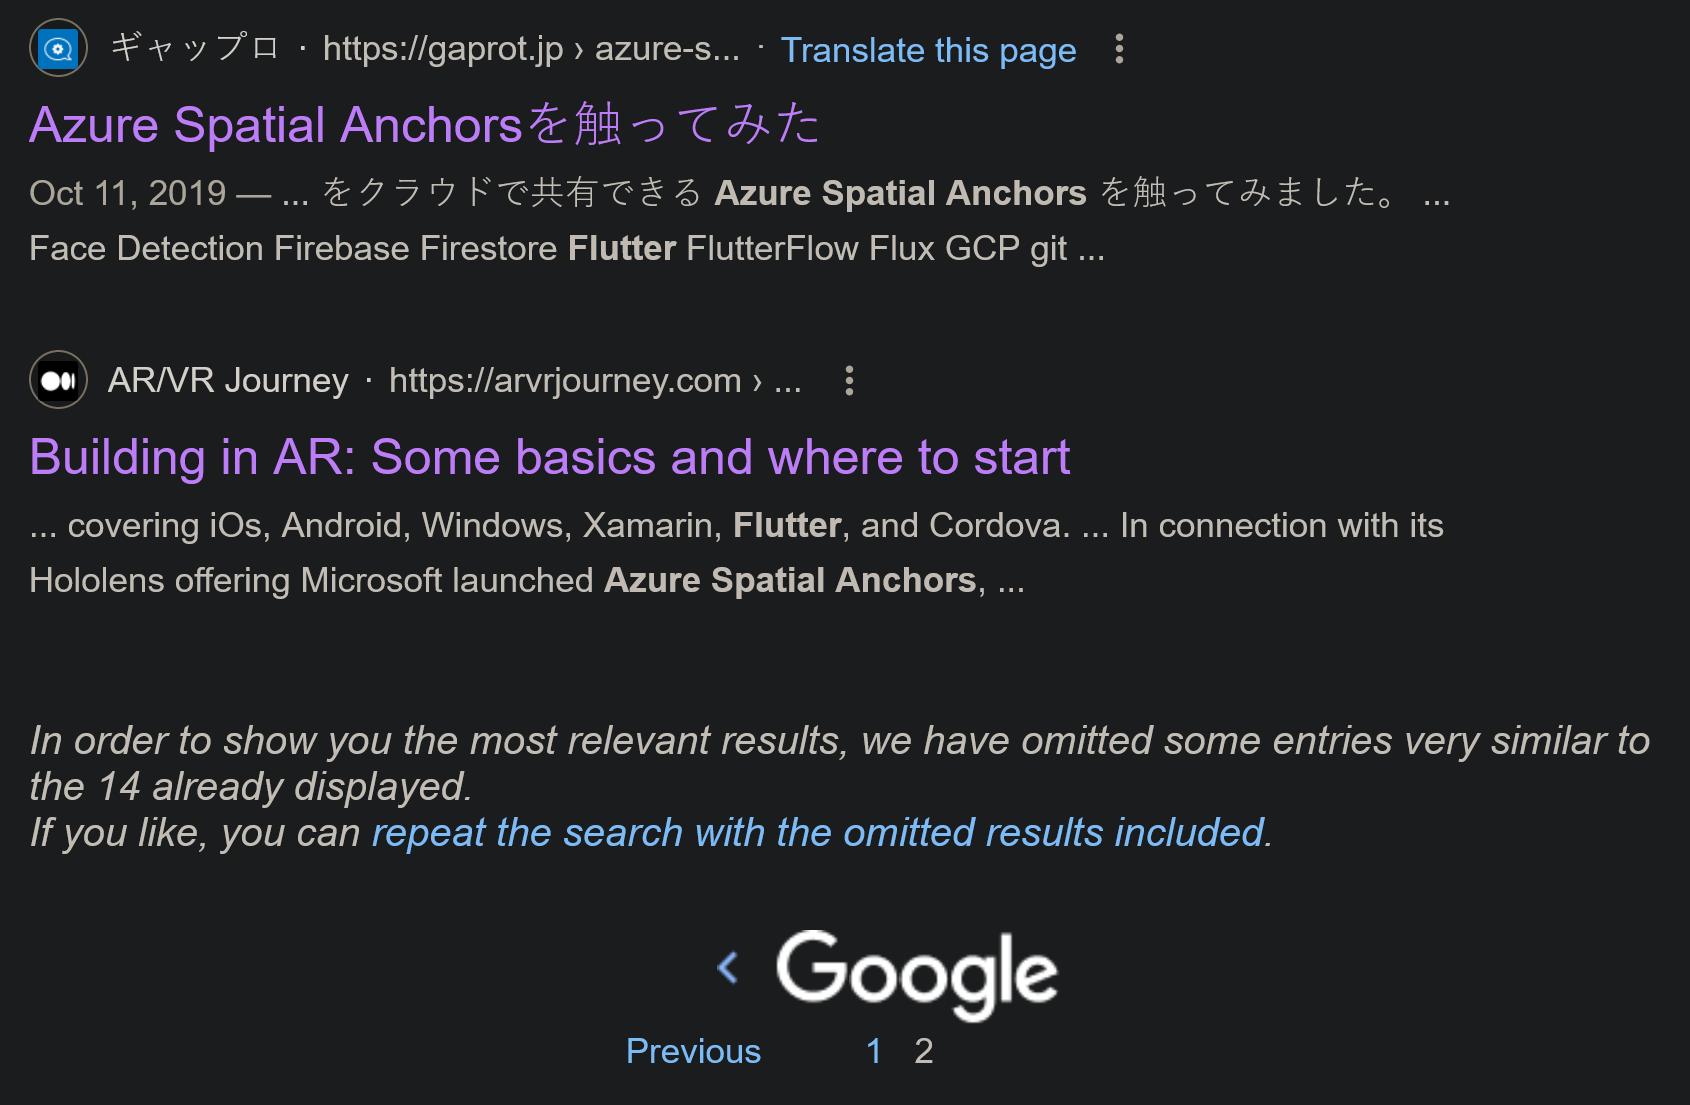
\includegraphics[width=.8\textwidth]{asa_flutter_search_today}
  \caption[Ricerca esatta Flutter e ASA 8 febbraio]{All'otto febbraio 2023 non si notano miglioramenti: solo 14 risultati rilevanti, alcuni in lingua giapponese, mostrano quando sia difficile trovare informazioni sull'argomento.}
  \label{fig:search2}
\end{figure}

Ho quindi dovuto, a causa di questa situazione, risolvere tutti i problemi incontrati senza poter fare affidamento su alcun aiuto esterno e questo ha esacerbato ulteriormente l'approccio \textit{trial-and-error} di cui si è parlato nella sezione \ref{sec:pianificazione}.

%************************************************************************************************************

\section{Raggiungimento obiettivi}
\subsection{Raggiungimento obiettivi proponente}
Riprendo quanto riportato in sezione \ref{sec:obiettivi} per trarre un bilancio sul grado di soddisfacimento dell'azienda nei confronti dei risultati ottenuti nel corso dello \textit{stage}, che schematizzo di seguito (riportando obiettivo, se è stato raggiunto e dove trovarne la prova).

\aCapo{}
\textbf{Obiettivi minimi:}

{
    \setlength{\freewidth}{\dimexpr\textwidth-10\tabcolsep}
    \renewcommand{\arraystretch}{1.5}
    \centering
    \setlength{\aboverulesep}{0pt}
    \setlength{\belowrulesep}{0pt}
    \rowcolors{2}{red!10}{white}
    \begin{longtable}{C{.8\freewidth} C{.162\freewidth} C{.115\freewidth}}
       \toprule
    \rowcolor{red}
    \textcolor{white}{\textbf{Obiettivo}}&
    \textcolor{white}{\textbf{Raggiunto}}&
    \textcolor{white}{\textbf{Fonte}}\\
    \toprule
    \endhead
    
    Studio e comprensione del linguaggio di programmazione Dart e del \textit{framework} Flutter & \cellcolor{green!20}SI & \ref{ch:flutter}\\
    Analisi strumenti Azure: Azure Console e \asa{}& \cellcolor{green!20}SI & \ref{subsec:azure}\\
    Ricerca di \textit{framework} e \sdk{} per implementare le \asa{} in Flutter& \cellcolor{green!20}SI & \ref{subsec:framework_ar}\\
    Eventuale studio di linguaggi necessari alle implementazioni native, come ad esempio Kotlin, Java, Unity o Swift & \cellcolor{green!20}SI & \ref{lst:android_channels}, \ref{lst:ios_channels}.\\
    Completamento del \textit{framework} scelto nell'app Flutter esistente& \cellcolor{green!20}SI &\ref{lst:mobilesyn_managers}, \ref{lst:arplug_manager} \\
    Completamento dello sviluppo dei componenti per rappresentare le \textit{anchor} nello spazio in realtà aumentata& \cellcolor{green!20}SI & \ref{lst:ar_view}\\
    Completamento dello sviluppo delle \api{} per l'interazione utente con gli ancoraggi in realtà aumentata& \cellcolor{green!20}SI & \ref{lst:mobilesyn_asset_provider}, \ref{lst:mobilesyn_ticket_provider}, \ref{lst:mobilesyn_asset_ticket_provider}\\

    \bottomrule
    \rowcolor{white} 
    \caption{Tabella dei requisiti funzionali}
    \end{longtable}
}

\aCapo{}
\textbf{Obiettivi massimi:}

{
    \setlength{\freewidth}{\dimexpr\textwidth-10\tabcolsep}
    \renewcommand{\arraystretch}{1.5}
    \centering
    \setlength{\aboverulesep}{0pt}
    \setlength{\belowrulesep}{0pt}
    \rowcolors{2}{red!10}{white}
    \begin{longtable}{C{.8\freewidth} C{.162\freewidth} C{.115\freewidth}}
       \toprule
    \rowcolor{red}
    \textcolor{white}{\textbf{Obiettivo}}&
    \textcolor{white}{\textbf{Raggiunto}}&
    \textcolor{white}{\textbf{Fonte}}\\
    \toprule
    \endhead
    
    Sviluppo di componenti per mappare \textit{asset} aziendali ad \textit{anchor} & \cellcolor{green!20}SI & \ref{fig:place_asset}\\
    Sviluppo di componenti grafici per la visualizzazione di metriche e informazioni di controllo& \cellcolor{red!20}NO & \\

    \bottomrule
    \rowcolor{white} 
    \caption{Tabella dei requisiti funzionali}
    \end{longtable}
}
Complessivamente ritengo di aver soddisfatto gli obiettivi posti dal proponente con un buon grado di completezza.

\subsection{Raggiungimento obiettivi personali}
Riprendendo quanto detto in sezione \ref{sec:motivazione_scelta} traggo un bilancio sul mio grado di soddisfacimento personale rispetto allo \textit{stage} svolto.

\begin{itemize}
  \item Acquisire competenze di programmazione \textit{frontend}:
      \begin{itemize}
          \item Utilizzare linguaggi specifici (ad esempio Dart);
          \item Sviluppare componenti grafiche per applicazioni \textit{mobile};
          \item Sviluppare familiarità con strumenti comunemente usati (ad esempio \vsc);
      \end{itemize}
\end{itemize}

Questo primo obiettivo l'ho soddisfatto quasi nella sua interezza: ho avuto modo di sviluppare con Dart e ho usato estensivamente \vsc{} e \astudio{}, tuttavia il lavoro nel suo complesso si è incentrato sull'infrastruttura sottostante piuttosto che sulla creazione di molteplici elementi grafici e quindi la sensazione di aver "creato un'applicazione", o meglio di aver lavorato sul \textit{fronted} piuttosto che sul \textit{backend}, è stata meno forte del previsto.

\begin{itemize}
  \item Osservare direttamente il lavoro in azienda \textit{software}:
    \begin{itemize}
        \item Vedere organizzazione giornaliera lavori;
        \item Valutare tempistiche e ritmi lavorativi;
        \item Valutare equilibrio vita-lavoro;
    \end{itemize}
\end{itemize}

Il secondo obiettivo l'ho completamente soddisfatto: ho potuto vedere i ritmi lavorativi all'interno dell'ufficio e farmi un'idea molto più chiara di cosa aspettarmi una volta uscito dal cammino universitario.\\
Inoltre, complice un'organizzazione settimanale che ha compreso tre giorni in presenza e tre giorni di lavoro a distanza, ho avuto un'impressione nel complesso positiva di quello che è l'equilibrio vita-lavoro in ambiente aziendale (o perlomeno in ambiente di \textit{startup}).\\


\begin{itemize}
  \item Acquisire competenze di sviluppo \textit{mobile}:
        \begin{itemize}
            \item Sviluppare familiarità con strumenti comunemente usati (ad esempio emulatori);
            \item Sviluppare componenti applicazione \textit{mobile};
            \item Utilizzare \textit{framework} specifici (ad esempio Flutter);
        \end{itemize}
\end{itemize}

Il terzo obiettivo l'ho completamente soddisfatto: ho avuto modo di sviluppare e provare applicazioni costruite in Flutter sia su emulatore che sul mio telefono personale, usando strumenti specifici com \astudio{} o i vari \textit{plugin} di Flutter per \vsc{}.

\begin{itemize}
  \item Acquisire competenze di realtà aumentata:
        \begin{itemize}
            \item Comprendere teoria dietro concetti come ancoraggi e tridimensionalità;
            \item Conoscere tecnologie principali usate nel campo;
            \item Valutare se sia di mio interesse perseguire studi futuri sull'argomento.
        \end{itemize}
\end{itemize}

Il quarto obiettivo l'ho soddisfatto a un livello che ritengo soddisfacente: ho avuto modo di usare un sottoinsieme rilevante delle maggiori tecnologie per la realtà aumentata (ARCore, ARKit e \asa{}) e ne ho studiato la teoria sottostante. Sebbene abbia ancora qualche riserva sull'uso di queste risorse in ambito professionale, ritengo abbiano un grande potenziale.\\
Nel complesso ritengo questa esperienza di \textit{stage} più che positiva e arricchente da un punto di vista sia tecnico che professionale.

\section{Competenze}
Durante questo stage ho acquisito o affinato un discreto insieme di competenze, a partire da linguaggi mai usati prima (Dart, Kotlin e Swift) per passare allo sviluppo nel \textit{framework} Flutter fino ad arrivare all'uso del \textit{sdk} \asa{}.\\
Ho imparato a comprendere e sfruttare codice di terze parti, preso da \textit{repository} e quindi affinando la mia comprensione dello strumento GitHub, e a destreggiarmi in mancanza di documentazione o direzioni esplicite.\\
Ho sviluppato componenti grafiche e in generale componenti per applicazioni \textit{mobile} \textit{frontend} e ho acquisito una maggiore dimestichezza con degli \ide{} largamente usati, ovvero \vsc{}, \astudio{} e Xcode.\\
Inoltre mi sono trovato a dover gestire l'interoperabilità tra linguaggi diversi ed effettuare operazioni di \textit{debugging} sfruttando i \textit{logs} dell'applicazione.\\
Per schematizzare:

\begin{itemize}
  \item Uso dei linguaggi:
      \begin{itemize}
        \item Dart;
        \item Kotlin;
        \item Java;
        \item Swift;
      \end{itemize}
  \item Uso del \textit{framework} Flutter;
  \item Utilizzo degli \ide{}s:
      \begin{itemize}
        \item \vsc{};
        \item \astudio{};
        \item Xcode;
      \end{itemize}
  \item Competenze di programmazione \textit{frontend} e \textit{mobile}:
      \begin{itemize}
        \item Sviluppo componenti grafiche;
        \item Sviluppo componenti di infrastruttura;
      \end{itemize}
  \item Competenze teoriche su tecnologie per realtà aumentata:
      \begin{itemize}
        \item ARCore;
        \item ARKit;
        \item \asa;
      \end{itemize}
  \item Uso di codice di terzi preso da \textit{repository} esterne;
  \item Gestione interoperabilità di codice scritto in linguaggi diversi;
  \item Lettura e comprensione dei \textit{logs} di \textit{debugging} per le applicazioni a \textit{runtime}.
\end{itemize}

Passando invece alle competenze delle quali mi sono scoperto manchevole, tralasciando le ovvie lacune sulle tecnologie tratte (come Flutter o \asa{}), quelle di cui ho più accusato l'assenza sono di natura più pratica che teorica: infatti non ero abituato a gestire codice di terzi, preso da \textit{repository}, leggerlo e integrarlo nel mio programma. Così come non mi era ancora capitato di gestire l'interoperabilità di linguaggi diversi per raggiungere un fine.\\
Queste lacune sono facilmente reinterpretabili in una critica al corso di studi, che forse lascia troppo poco spazio all'effettivo lavoro di progettazione e codifica in favore di un approccio più teorico.\\
Un modo per arginare il problema sarebbe potenziare le attività didattiche pratiche (comunque presenti, come gli \textit{assignment} dei corsi di Programmazione ad Oggetti e Tecnologie Web o il progetto del corso di Ingegneria del Software) a discapito di quelle più teoriche (come Calcolo Numerico o Logica).


\iffalse
% !TEX encoding = UTF-8
% !TEX TS-program = pdflatex
% !TEX root = ../tesi.tex

%**************************************************************
\chapter{Introduzione}
\label{cap:introduzione}
%**************************************************************

\section{L'azienda}
\begin{figure}[ht]
    \centering
    
\includegraphics[height=3cm]{ds_logo}
    \caption{Logo Datasoil S.r.l.}
\end{figure}

Datasoil S.r.l. è una startup innovativa che investe nel capitale umano al fine di formare sviluppatori che riescano a prendere decisioni e responsabilità di progetto avanzate. La loro mission è quella di impiegare tecnologie sempre più innovative e portare novità ai loro clienti. \\Per questi motivi i nuovi sviluppatori junior saranno sempre inseriti su progetti/prodotti core dell’azienda e seguiti da sviluppatori senior full time sulle attività di formazione, progettazione e chiarimenti nel day to day.\\
Datasoil S.r.l. sviluppa piattaforme per l’industry 4.0 che permettono di fondere le informazioni e gli eventi provenienti da diversi livelli aziendali per creare insight proattivi integrati in tempo reale. Ogni evento, che sia un malfunzionamento o un'eccezione segnalata da altri operatori, viene notificato alla persona giusta al momento giusto anticipando la gestione delle criticità interfunzionali.\\
Inoltre, in quest'ultimi anni di pandemia, Datasoil S.r.l. ha deciso di sfruttare la competenza dei loro dipendenti per aiutare le aziende a garantire la sicurezza dei lavoratori. Per fare ciò sono stati utilizzati degli smartband, i quali permettono il tracciamento completamente anonimo dei contatti a rischio e garantiscono il rispetto del distanziamento sociale. Nel pieno rispetto della privacy e GDPR gli individui a rischio vengono avvisati da una vibrazione del braccialetto nel caso di contagio.

%**************************************************************
\section{Il progetto e lo stage}

\subsection{Descrizione}
Il progetto proposto prevede l’implementazione di due applicazioni mobile multipiattaforma: \textbf{LifestyleSync} e \textbf{LSCoach}.\\
\textbf{LifestyleSync}, legata al mondo wellness/fitness, serve come supporto della piattaforma di analisi dati realizzata per un prodotto spinoff di Datasoil. \\
L'idea alla base del progetto è quella di fornire uno strumento per migliorare il benessere dei propri dipendenti alle aziende.\\
Grazie a questo prodotto ogni dipendente, o cliente, sarà seguito da un coach che lo aiuterà a mantenersi in forma, sia tramite obiettivi di movimento ed allenamento, sia tramite obiettivi alimentari, inoltre i parametri di salute del cliente saranno rilevati e trasmessi al proprio coach in modo da predisporre allenamenti personalizzati. \\
Lo scopo dell'applicazione è quello di fornire un'interfaccia mobile ai clienti, interfaccia tramite la quale potranno interagire con il proprio coach, visualizzare gli obiettivi a loro assegnati, gli appuntamenti e il loro percorso a livello di fitness.\\
Per garantire al coach la possibilità di prestare i propri servizi ai clienti in modo unificato, si è resa necessaria la progettazione di una seconda applicazione specifica: \textbf{LSCoach}. Il coach potrà vedere i suoi appuntamenti con i clienti, lo stato di forma e gli obiettivi assegnati ad ogni cliente.

\subsection{Obiettivi}
\begin{itemize}
    \item Studio e comprensione del linguaggio di programmazione \textit{Dart} e del framework \textit{Flutter};
    \item Progettazione, completo sviluppo e verifica delle funzionalità di onboarding e primo login dell'app cliente: breve introduzione all'uso dell'applicazione, sistema di autenticazione e questionario conoscitivo;
    \item Progettazione, completo sviluppo e verifica delle funzionalità di connessione ai device dell'utente dell'app cliente: connessione ai profili fitness Google Fit, Fitbit e Garmin per il rilevamento di dati;
    \item Progettazione, sviluppo e verifica delle funzionalità individuate per la dashboard utente dell'app cliente: obiettivi di movimenti, lista degli obiettivi raggiunti e falliti, agenda con gli appuntamenti, pagina del profilo con calcolo del \gls{BMI};
    \item Progettazione, inizio dello sviluppo e verifica delle funzionalità principali per l'applicazione dei coach: visualizzazione dei clienti con i relativi obiettivi in corso e agenda con gli appuntamenti.
\end{itemize}

\subsection{Pianificazione del lavoro}
\begin{itemize}
    \item \textbf{Settimana 1:} configurazione dell'ambiente di lavoro e studio di Flutter;
    \item \textbf{Settimana 2:} progettazione e sviluppo delle prime funzionalità onboarding: introduzione all'applicazione;
    \item \textbf{Settimana 3:} implementazione del login tramite auth0, progettazione e sviluppo del sondaggio iniziale;
    \item \textbf{Settimana 4:} progettazione e sviluppo delle prime schermate di dashboard utente: Homepage, Device Connection e Profilo;
    \item \textbf{Settimana 5:} progettazione e sviluppo di ulteriori schermate: Obiettivi con dettaglio, appuntamenti con dettaglio;
    \item \textbf{Settimana 6:} progettazione e sviluppo della agenda con i relativi impegni settimanali e mensili;
    \item \textbf{Settimana 7:} testing di diversi sdk per l'implementazione di una chat, progettazione e sviluppo app coach;
    \item \textbf{Settimana 8:} progettazione e sviluppo di un sistema di notifiche push con l'utilizzo di Google Firebase;
    \item \textbf{Settimana 9:} raffinamento e completamento delle funzionalità precedentemente sviluppate.
\end{itemize}

%************************************************************************************************************
\section{Prodotto ottenuto}
Il prodotto ottenuto si compone di due diverse applicazioni: applicazione cliente e applicazione coach.\\
Entrambe le applicazioni sono state sviluppate utilizzando \textit{Flutter} come framework in modo da valutarne anche le potenzialità, infatti l'azienda ha sempre utilizzato React Native per lo sviluppo mobile. Mentre per lo stile dei componenti dell'applicazione si è deciso di utilizzare il \textit{Material Design} di Google già ampiamente utilizzato da Datasoil S.r.l.\\
L'applicazione cliente allo stato attuale permette la visione dei propri obiettivi di movimento e degli appuntamenti, oltre che una schermata di profilo personale con la possibilità di associazione ai diversi profili fitness al fine di rilevare dati.\\
L'app cliente è quindi a circa un terzo dello sviluppo, l'azienda ora potrà continuare con lo sviluppo delle restanti sezioni relative alla dieta e alla visualizzazione dello stato di salute del cliente. \\
L'applicazione coach allo stato attuale permette la visualizzazione della lista dei propri clienti con i relativi obiettivi di movimento e la visualizzazione di un'agenda con gli appuntamenti. L'app coach è in buona parte sviluppata, l'idea aziendale è quella che dall'app il coach possa solo vedere ciò che ha già assegnato dall'interfaccia web (prodotto già sviluppato da Datasoil S.r.l.). \\
L'azienda quindi dovrà solo aggiungere la visualizzazione della dieta e dei parametri di salute del cliente, omettendo la possibilità di assegnare ulteriori obiettivi dall'app mobile. 
Per entrambe le applicazioni è stata predisposta una versione minimale di chat in modo che il cliente possa comunicare con il proprio coach. Questa chat sarà in futuro ampiamente rivista in modo da permettere lo scambio di file multimediali e di video chiamate, oltre che limitare lo scambio di messaggi tramite una sorta di abbonamento.
%************************************************************************************************************
\section{Difficoltà incontrate}
La principale difficoltà incontrata durante lo svolgimento del progetto è stata l'apprendimento del linguaggio di programmazione \textit{Dart} e soprattutto del framework \textbf{Flutter}.\\
Flutter permette di scrivere in modo semplice applicazioni mobile multipiattaforma.\\
Flutter è un framework più performante di React Native in termini di \textit{rendering} UI, ma allo stesso tempo, vista la sua recente esplosione è ancora poco conosciuto e la documentazione online non è troppo vasta.\\ 
Per superare questa difficoltà è servito un breve periodo di studio del framework seguendo le guide presenti nel suo sito e la codifica di diverse applicazioni demo.\\
Un'altra difficoltà è stato l'apprendimento e la progettazione delle questioni \textit{core} dell'applicazione, come la gestione delle richieste asincrone al backend, la gestione degli errori e la gestione dello stato dell'applicazione.\\
La soluzione a questa difficoltà è stata la comunicazione frequente con il mio tutor, il quale ha chiarito i miei dubbi principali e mi ha consigliato delle applicazioni demo da sviluppare per assodare i concetti.\\
Un altro problema è sorto durante lo sviluppo, alcune librerie che si intendeva utilizzare avevano bisogno di alcune migliorie e correzione di bug. È stato quindi necessario fare un \gls{fork} alle librerie in questione ed effettuare le diverse modifiche necessarie.\\
Un'altra difficoltà è sorta nelle ultime settimane: si è deciso di sviluppare una seconda applicazione da utilizzare a lato coach riutilizzando buona parte dei componenti già sviluppati per i clienti.\\
La difficoltà è stata quella di rendere questi componenti parametrizzabili e di rivedere interamente la struttura della \textit{repository}, oltre che impostare le corrette configurazioni in modo da poter compilare due diverse applicazioni utilizzando dei file in comune.

%**************************************************************
\section{Struttura della relazione}

\begin{description}
    \item[{\hyperref[cap:strumenti-utilizzati]{Il secondo capitolo}}] descrive gli strumenti e le tecnologie utilizzate per svolgere il progetto, particolare attenzione è posta sulla presentazione del framework Flutter, in quanto è alla base del prodotto ottenuto;
    
    \item[{\hyperref[cap:analisi-requisiti]{Il terzo capitolo}}] espone un'analisi tecnica dei requisiti individuati che il prodotto finale deve soddisfare al termine del periodo di stage;
    
    \item[{\hyperref[cap:progettazione]{Il quarto capitolo}}] descrive le scelte progettuali adottate per ottenere una struttura solida manutenibile;
    
    \item[{\hyperref[cap:sviluppo]{Il quinto capitolo}}] espone il percorso di realizzazione del prodotto e le soluzioni alle difficoltà incontrate;
    
    \item[{\hyperref[cap:conclusioni]{Il sesto capitolo}}] descrive l'esperienza di stage e i risultati ottenuti.
\end{description}

Riguardo la stesura del testo, relativamente al documento sono state adottate le seguenti convenzioni tipografiche:
\begin{itemize}
	\item gli acronimi, le abbreviazioni e i termini ambigui o di uso non comune menzionati vengono definiti nel glossario, situato alla fine del presente documento;
	\item i termini in lingua straniera o facenti parti del gergo tecnico sono evidenziati con il carattere \emph{corsivo}.
\end{itemize}             % Introduzione
% !TEX encoding = UTF-8
% !TEX TS-program = pdflatex
% !TEX root = ../tesi.tex

%**************************************************************
\chapter{Strumenti utilizzati}
\label{cap:strumenti-utilizzati}
%**************************************************************

\section{Strumenti di sviluppo}
\subsection{Visual Studio Code}
\begin{figure}[ht]
    \centering
    
\includegraphics[height=2cm]{vsc_logo}
    \caption{Logo di Visual Studio Code}
\end{figure} \aCapo{}
\vsc{} è un editor per codice sorgente, sviluppato da \textit{Microsoft} servendosi del framework \textit{Electron}, disponibile per Windows, Linux e macOS. Le sue funzionalità comprendo supporto per debugging, syntax highlighting, intelligent code completion, snippets, code refactoring, e integrazione con Git. \\
Gli utenti possono configurare tema, macro, preferenze e installare estensioni che ne aumentano le funzionalità aggiungendo ad esempio il supporto ai maggiori linguaggi di porgrammazione attualmente presenti.\\
Nella \textit{Stack Overflow 2021 Developer Survey}, \vsc{} è risultato essere l'IDE più popolare, adottato dal 70\% degli intervistati. {\tiny Fonte: \href{https://en.wikipedia.org/wiki/Visual_Studio_Code}{Wikipedia}}\\
\E{} inoltre presente e molto comoda l'estensione di \flutter{} che, tra le altre cose, permette di gestire direttamente in gui i vari dispositivi (smartphone, browser o emulatore) sui quali installare e lanciare l'app che si sta programmando.

\subsection{Android Studio}
\begin{figure}[ht]
    \centering
    
\includegraphics[height=2cm]{as_logo}
    \caption{Logo di Android Studio}
\end{figure}\aCapo{}
\textit{Android Studio} è l'IDE ufficiale del sistema operativo di Gooogle, sostituendo Eclipse dal 2015, costruito sul software IntelliJ di JetBrains e progettato specificatamente per lo sviluppo Android. \E{} disponibile per Windows, Linux e macOS.\\
Il 7 maggio 2019 Kotlin rimpiazzò Java come linguaggio consigliato per Android, favorendo un'integrazione ancora maggiore con JetBrains che, appunto, ha sviluppato e prodotto Kotlin stesso. {\tiny Fonte: \href{https://en.wikipedia.org/wiki/Android_Studio}{Wikipedia}}\\
Personalmente ho cercato nonostante tutto di programmare il più possibile su \vsc{} preferendolo quindi ad \textit{Android Studio} in virtù della sua maggiore leggerezza e delle sue più ampie possibilità di personalizzazione.

\subsection{Dart}
\begin{figure}[ht]
    \centering
    
\includegraphics[height=2cm]{dart_logo}
    \caption{Logo di Dart}
\end{figure} \aCapo{}
Dart è un linguaggio di programmazione sviluppato da Google per il client development, ovvero per web e mobile app, e può anche essere impiegato per la costruzione di applicazione desktop e server.\\
\E{} un linguaggio object-oriented, class-based, garbage-collected, strongly-typed e con una sintassi nello stile di C. Può compilare sia codice macchina che JavaScript e supporta interefacce, mixins, classi astratte, refined generics e type inference.{\tiny Fonte: \href{https://en.wikipedia.org/wiki/Dart_(programming_language)}{Wikipedia}}\\
Personalmente l'ho trovato elegante e conciso nella sua struttura, e presenta dei vantaggi consistenti come la null protection e le espressioni ternarie.

\subsection{Flutter}
\begin{figure}[ht]
    \centering
    
\includegraphics[height=2cm]{flutter_logo}
    \caption{Logo di Flutter}
\end{figure} \aCapo{}
Flutter è un framework open-source creato da Google per lo sviluppo della UI di applicazioni cross-platform per Android, iOS, Linux, macOS, Windows, Google Fuchsia e il web partendo da un singolo codebase.\\
Rialsciato a maggio 2017, le applicazioni in Flutter sono scritte in Dart e sfruttano molte delle features avanzate del linguaggio, e le componenti principali del framework sono:
\begin{itemize}
    \item \textbf{Dart platform:} Flutter gira all'interno della Dart Virtual Machine, che si serve di un execution engine just-in-time;
    \item \textbf{Flutter engine:} scritto primariamente in C++, fornisce supporto a basso livello per il rendering e implementa accessibilità, file e network I/O, supporto nativo per i plugin e molto altro;
    \item \textbf{Foundation library:} scritta in Dart, fornisce classi e funzioni di base che vengono usate per costruire gli applcativi in Flutter, come ad esempio le API per la comunicazione con l'engine;
    \item \textbf{Design-specific widgets:} Flutter contiene due famiglie di widget che si conformano a delle specifiche scuole di design: \textit{Material} per Google e \textit{Cupertino} per Apple;
    \item \textbf{Flutter DevTools:} famiglia di tools generici che vengono sfruttati per lo sviluppo di software in Flutter.
\end{itemize}
~\\
Inoltre, una libreria fondamentale per semplificare l'utilizzo di Flutter è \textit{Flutter Hooks}: lo scopo è implementare delle strutture simili agli Hooks di React, consentono di sostituire gli Stateful Widget riducendo il boilerplate code e semplificando la gestione di side-effect e ciclo di vita dei widget grazie alla funzione \textit{useEffect}.

\subsection{Java}
\begin{figure}[ht]
    \centering
    
\includegraphics[height=4cm]{java_logo.png}
    \caption{Logo di Java}
\end{figure} \aCapo{}
Java è un linguaggio di programmazione ad alto livello object-oriented progettato per avere il minor numero possibile di dipendenze implementative (favorendo quindi l'uso di interfacce e classi astratte) e, soprattutto, per aderire al motto \textit{"write once, run anywhere"}: il bytecode di Java può infatti girare senza necessità di ricompilazione su qualsiasi piattaforma che supporti la Java Virtual Machine (comunemente abbreviata in JVM).\\  
La sintassi è simile a quelle di C o C++, ma fornisce funzionalità dinamiche generalmente inedite per i linguaggi compilati, come reflection e modifica del codice a runtime.\\
Originalmente rilasciato nel 1995 come componente centrale della piattaforma Java per Sun Microsystems e sotto licenza proprietaria, dal 2007 la maggior parte dei suoi componenti sono diventati open-source sotto l'ombrello della \textit{GPL-2.0-only} (licenza specifica per software libero pubblicata dalla Free Software Foundation).\\
Sebbene Oracle (attuale proprietario di Sun Microsystems) offra un'implementazione proprietaria chiamata \textit{HotSpot JVM}, la specifica ufficiale è la \textit{OpenJDK JVM} che è gratuita, open-source e di default nella maggior parte delle distribuzioni Linux.

\subsection{Kotlin}
\begin{figure}[ht]
    \centering
    
\includegraphics[height=1.5cm]{kotlin_logo.png}
    \caption{Logo di Kotlin}
\end{figure} \aCapo{}
Kotlin è un linguaggio di programmazione cross-platform, staticamente tipizzato, progettato per avere completa interoperabilità con Java, gode di una sintassi più concisa di quest'ultimo grazie alla type inference di cui è dotato e dipende dalla \textit{Java Class Library} per la versione della JVM da usare.\\
\E{} inoltre in grado di compilare codice in JavaScript (sfruttato poi da applicazioni frontend) o codice nativo tramite \textit{LLVM} (per app iOS che condividono la business logic con applicazioni Android).\\
Incluso in Android Studio come alternativa al compilatore standard Java dal 2017, produce bytecode Java 8 di default ma permette al programmatore di scegliere delle versioni target successive (fino a Java 18).

\subsection{Azure Spatial Anchors}
\begin{figure}[ht]
    \centering
    
\includegraphics[height=2.5cm]{asa_logo.png}
    \caption{Logo di Azure Spatial Anchors}
\end{figure} \aCapo{}
Azure Spatial Anchors è un servizio di Microsoft mirato a fornire strumenti per sviluppare applicazioni in realtà aumentata su dispositivi iOS o Android predisposti per, rispettivamente, ARKit e ARCore, oppure su Microsoft HoloLens.\\
Permette di riconoscere spazi tridimensionali all'interno dei quali posizionare punti di interesse, chiamati Spatial Anchors, che possono essere salvati in cloud e poi recuperati, e possono essere messi in relazione a oggetti reali (come macchinari in un contesto industriale) o virtuali.

\subsection{ARCore}
\begin{figure}[ht]
    \centering
    
\includegraphics[height=2cm]{arcore_logo.png}
    \caption{Logo di ARCore}
\end{figure} \aCapo{}
ARCore, conosciuto anche come Google Play Services per AR, è un software development kit prodotto da Google per permettere lo sviluppo di applicazioni in realtà aumentata.\\
Si serve di tre componenti principali:
\begin{itemize}
    \item \textbf{6DOF:} il dispositivo sfrutta una piattaforma inerziale a sei assi per comprendere e tracciare la propria posizione relativa allo spazio;
    \item \textbf{Environmental understanding:} permette riconoscere dimensioni e locazione delle superfici lisce;
    \item \textbf{Light estimation:} permette al telefono di stimare le condizioni di luce dell'ambiente.
\end{itemize}
asa si appoggia proprio ad ARCore per implementare le proprie funzionalità di AR su Android.

\todo
\textcolor{todoOrange}{ar flutter plugin, sceneform?}


%**************************************************************
\section{Strumenti organizzativi}

\subsection{Slack}
\begin{figure}[ht]
    \centering
    
\includegraphics[height=1.5cm]{slack_logo}
    \caption{Logo di Slack}
\end{figure}
Slack è una piattaforma di comunicazione istantanea di proprietà di Salesforce e sviluppata da Slack Technologies per Windows, Linux, macOS, Android e iOS.\\
Permette di comunicare tramite messaggi, chiamate vocali e video, e di inviare media e files nelle chat private o nei canali. Quest'ultimi fungono da aggregatori e permettono di suddividere tematicamente la comunicazione.\\
\E{} inoltre possibile suddividere a un livello ancora più alto tramite i \textit{workspaces}, che aggregano al proprio interno utenti, canali e applicazioni: sono proprio quest'ultime che mostrano con maggiore chiarezza l'orientamento \textit{corporate} di Slack, infatti fornisce integrazione nativa con i maggiori software gestionali e organizzativi (come ad esempio Jira, Zoom, Drive, Outlook, etc).

\subsection{Github}
\begin{figure}[ht]
    \centering
    
\includegraphics[height=3cm]{github_logo}
    \caption{Logo di GitHub}
\end{figure}
GitHub è il più grande servizio di hosting di codice sorgente al mondo, abitualmente usato per sviluppare progetti open source, e fornisce vari servizi: version control di Git distribuito e access control, bug tracking, issue tracking, richieste di modifiche software, task management, integrazione continua e wiki per ogni progetto.\\ 
Permette inoltre, tramite forking, pull request e commenti, il miglioramento collaborativo del software, ad esempio risolvendo bug, aggiungendo funzionalità o migliorando quelle presenti.

             % Processi
% !TEX encoding = UTF-8
% !TEX TS-program = pdflatex
% !TEX root = ../tesi.tex

%**************************************************************
\chapter{Analisi dei requisiti}
\label{cap:analisi-requisiti}
%**************************************************************

\section{Requisiti individuati}

I requisiti individuati a partire dal problema proposto e dalle discussioni con il tutor aziendale sono stati catalogati secondo il codice:\\
\begin{center}
    \textbf{R[Importanza][Tipo][Codice]}
\end{center}
dove:
\begin{itemize}
    \item Importanza: specifica l'importanza del requisito e può assumere i seguenti valori:
    \begin{itemize}
        \item \textbf{1: } Requisito obbligatorio;
        \item \textbf{2: } Requisito desiderabile ma non essenziale per il funzionamento;
        \item \textbf{3: } Requisito opzionale.
    \end{itemize}
    \item Tipologia: specifica la tipologia del requisito e può assumere i seguenti valori:
    \begin{itemize}
        \item \textbf{F: }\textit{funzionale,} cioè determina una funzionalità dell'applicazione;
        \item \textbf{V: }\textit{vincolo,} che riguarda un vincolo che il prodotto deve rispettare.
    \end{itemize}
    \item Codice: identificativo univoco del requisito espresso in forma gerarchica padre/figlio.
\end{itemize}

\subsection{Requisiti app cliente}

\setlength\arrayrulewidth{1pt}
\renewcommand{\arraystretch}{1.5}
\begin{longtable}{| c | C{10cm}|}
\label{tab:requisiti-funzionali-cliente}

\cellcolor{red}\textcolor{white}{\textbf{Requisito}} & \cellcolor{red}\textcolor{white}{\textbf{Descrizione}}\\\hline
\endhead
R1F1 & L'utente può utilizzare l'applicazione solo se autenticato\\\hline
R1F2 & Al primo accesso deve essere presentata una breve descrizione dell'applicazione.\\\hline
R1F3 & Al primo accesso deve essere presentato all'utente il suo coach.\\\hline
R1F4 & Al primo accesso l'utente deve compilare un questionario.\\\hline
R1F5 & L'utente deve poter effettuare il logout dall'applicazione.\\\hline
R1F6 & L'utente deve poter vedere il totale dei suoi minuti attivi settimanali.\\\hline
R1F6.1 & L'utente deve poter vedere il totale dei suoi minuti attivi di attività settimanali.\\\hline
R1F6.2 & L'utente deve poter vedere il totale dei suoi minuti attivi non programmati settimanali.\\\hline
R1F6.3 & L’utente deve poter analizzare un confronto tra i suoi minuti attivi e il target stabilito dall’OMS \\\hline
R1F7 & L’utente deve poter vedere la lista dei suoi obiettivi attivi in quel determinato momento. \\\hline
R1F7.1 & Per ogni voce di un obiettivo (calorie, passi, minuti di attività, minuti non programmati) deve essere mostrato il progresso.\\\hline
R1F7.2 & L’utente deve poter sapere in quanti giorni scade un dato obiettivo. \\\hline
R1F7.3 & Per ogni obiettivo l’utente deve poter vedere le informazioni in dettaglio.\\\hline
R1F8 & L’utente deve poter vedere gli obiettivi passati o non attivi. \\\hline
R1F8.1 & L’utente deve poter scegliere per quale periodo vedere gli obiettivi passati. \\\hline
R1F8.2 & L’utente deve poter scegliere per un dato periodo se vedere gli obiettivi passati raggiunti o falliti. \\\hline
R1F9 & L’utente deve poter vedere un riepilogo con il totale degli obiettivi completati, falliti e in corso. \\\hline
R1F10 & L’utente deve poter vedere una lista con i prossimi appuntamenti del mese. \\\hline
R1F10.1 & Per ogni appuntamento l’utente deve poter vedere data, ora, titolo e coach. \\\hline
R1F10.2 & Per ogni appuntamento l’utente dove poter vedere le informazioni in dettaglio. \\\hline
R1F11 & L’utente deve poter vedere un calendario in cui saranno presenti tutti i suoi obiettivi attivi e i suoi appuntamenti passati e prossimi.\\\hline
R1F11.1 & Per ogni giorno del calendario l’utente dove poter vedere una lista con gli obiettivi del giorno e gli appuntamenti del giorno.\\\hline
R1F12 & L’utente dove poter associare il suo account dell’app a diversi servizi di fitness. \\\hline
R1F12.1 & L'utente deve poter associare il suo account dell'app all'account di Google Fit \\\hline
R1F12.2 & L'utente deve poter associare il suo account dell'app all'account di Fitbit \\\hline
R1F12.3 & L'utente deve poter associare il suo account dell'app all'account di Garmin \\\hline
R1F13 & L’utente deve poter vedere una schermata con le sue informazioni. \\\hline
R1F13.1 & L’utente deve poter vedere la sua altezza, il suo peso, la sua età e il suo \gls{BMI}. \\\hline
R1F13.2 & Deve essere presente una tabella di spiegazione per il \gls{BMI}. \\\hline
R1F14 & L’utente deve poter vedere chi è il suo coach anche in seguito al primo accesso. \\\hline
R2F15 & L'utente deve essere avvisato al raggiungimento di determinati obiettivi tramite popup. \\\hline
R2F15.1 & Quando l'utente sblocca un achievement deve ricevere una notifica e vedere un popup.\\\hline
R2F15.2 & Quando l'utente completa un obiettivo deve ricevere una notifica e vedere un popup. \\\hline
R2F15.3 & Quando l'utente raggiunge i minuti attivi consigliati dall'OMS deve vedere un popup. \\\hline

\caption{Tabella del tracciamento dei requisti funzionali}
\end{longtable}

\setlength\arrayrulewidth{1pt}
\renewcommand{\arraystretch}{1.5}
\begin{longtable}{| c | C{10cm}|}
\label{tab:requisiti-vincolo-cliente}
\cellcolor{red}\textcolor{white}{\textbf{Requisito}} & \cellcolor{red}\textcolor{white}{\textbf{Descrizione}}\\ \hline
\endhead
R1V1 & L'applicazione deve essere sviluppata usando Flutter. \\\hline
R1V2 & L'applicazione deve funzionare completamente su dispositivi Android. \\\hline
R2V3 & L'applicazione deve funzionare completamente su dispositivi iOS. \\\hline
R1V4 & L'interfaccia deve essere facilmente fruibile. \\\hline
R2V5 & L'applicazione deve presentare elementi di \gls{gamification}.\\\hline
\caption{Tabella del tracciamento dei requisti vincolo}
\end{longtable}

\subsection{Requisiti app coach}

\setlength\arrayrulewidth{1pt}
\renewcommand{\arraystretch}{1.5}
\begin{longtable}{| c | C{10cm}|}
\label{tab:requisiti-funzionali-coach}

\cellcolor{red}\textcolor{white}{\textbf{Requisito}} & \cellcolor{red}\textcolor{white}{\textbf{Descrizione}}\\\hline
\endhead
R1F1 & Il coach può utilizzare l'applicazione solo se autenticato\\\hline
R1F2 & Il coach deve poter effettuare il logout dall'applicazione.\\\hline
R1F3 & Il coach deve poter vedere una lista con i prossimi appuntamenti del mese. \\\hline
R1F3.1 & Per ogni appuntamento il coach deve poter vedere data, ora, titolo e cliente. \\\hline
R1F3.2 & Per ogni appuntamento il coach dove poter vedere le informazioni in dettaglio. \\\hline
R1F4 & Il coach deve poter vedere un calendario in cui saranno presenti tutti i suoi appuntamenti passati e prossimi.\\\hline
R1F4.1 & Per ogni giorno del calendario il coach dove poter vedere una lista con gli appuntamenti del giorno.\\\hline
R1F5 & Il coach deve poter scegliere il tenant di cui vedere i clienti.\\\hline
R1F6 &Il coach deve poter vedere i dettagli di ogni cliente\\\hline
R1F6.1 & Per ogni cliente il coach deve poter vedere l’altezza, il peso, l’età e il suo \gls{BMI}\\\hline
R1F6.2 & Per ogni cliente il coach deve poter vedere gli obiettivi in corso a lui assegnati\\\hline
R1F6.3 & Per ogni clienti il coach deve poter vedere gli obiettivi passati a lui assegnati\\\hline


\caption{Tabella del tracciamento dei requisti funzionali}
\end{longtable}

\setlength\arrayrulewidth{1pt}
\renewcommand{\arraystretch}{1.5}
\begin{longtable}{| c | C{10cm}|}
\label{tab:requisiti-vincolo-coach}
\cellcolor{red}\textcolor{white}{\textbf{Requisito}} & \cellcolor{red}\textcolor{white}{\textbf{Descrizione}}\\ \hline
\endhead
R1V1 & L'applicazione deve essere sviluppata usando Flutter. \\\hline
R1V2 & L'applicazione deve funzionare completamente su dispositivi Android. \\\hline
R2V3 & L'applicazione deve funzionare completamente su dispositivi iOS. \\\hline
R1V4 & L'interfaccia deve essere facilmente fruibile. \\\hline
R2V5 & L'applicazione deve presentare elementi di \gls{gamification}.\\\hline
\caption{Tabella del tracciamento dei requisti vincolo}
\end{longtable}

\section{Riepilogo requisiti}
\subsection{Riepilogo requisiti app cliente}
In totale sono stati individuati 39 requisiti, ripartiti tra le varie tipologie secondo quanto riportato nelle seguenti tabelle.\\
\begin{center}
\begin{minipage}[c]{0.7\linewidth}
    \begin{small}
    \begin{longtable}{|c|c|}
    \hline
         \textbf{Importanza}& \# \\\hline
         Obbligatori & 33\\\hline
         Desiderabili & 6\\
         \hline
    \caption{Numero di requisiti per importanza app cliente}
    \label{tab:requisiti-importanza-cliente}
    \end{longtable}   
    \end{small}
\end{minipage}


\begin{minipage}[c]{0.7\linewidth}
    \begin{small}
    \begin{longtable}{|c|c|}
    \hline
         \textbf{Tipologia}& \# \\\hline
         Funzionali & 34\\\hline
         Vincolo & 5\\
         \hline
    \caption{Numero di requisiti per tipologia app cliente}
    \label{tab:requisiti-tipolgia-cliente}
    \end{longtable}   
    \end{small}
\end{minipage}
\end{center}
\subsection{Riepilogo requisiti app coach}
In totale sono stati individuati 17 requisiti, ripartiti tra le varie tipologie secondo quanto riportato nelle seguenti tabelle.\\
\begin{center}
\begin{minipage}[c]{0.7\linewidth}
    \begin{small}
    \begin{longtable}{|c|c|}
    \hline
         \textbf{Importanza}& \# \\\hline
         Obbligatori & 15\\\hline
         Desiderabili & 2\\
         \hline
    \caption{Numero di requisiti per importanza app coach}
    \label{tab:requisiti-importanza-coach}
    \end{longtable}   
    \end{small}
\end{minipage}


\begin{minipage}[c]{0.7\linewidth}
    \begin{small}
    \begin{longtable}{|c|c|}
    \hline
         \textbf{Tipologia}& \# \\\hline
         Funzionali & 12\\\hline
         Vincolo & 5\\
         \hline
    \caption{Numero di requisiti per tipologia app coach}
    \label{tab:requisiti-tipolgia-coach}
    \end{longtable}   
    \end{small}
\end{minipage}
\end{center}             % Kick-Off
% !TEX encoding = UTF-8
% !TEX TS-program = pdflatex
% !TEX root = ../tesi.tex

%**************************************************************
\chapter{Progettazione}
\label{cap:progettazione}
%**************************************************************
\section{Organizzazione repository e sistema di ticketing}
\label{sec:organizzazione-repository-sistema-ticketing}

A livello di organizzazione del repository si è deciso di adottare lo stile generalmente utilizzato dall'azienda.\\
Partendo da una base stabile dell'applicazione si procede in modo incrementale per aggiunta di funzionalità seguendo un approccio \gls{agile}.\\
Ogni nuova funzionalità o \textit{issue} viene segnalata attraverso Jira da un membro del team, il quale si occupa anche di fornire un titolo, una breve descrizione e di assegnarla ad uno sviluppatore frontend o backend, in base al tipo di funzionalità. Jira automaticamente crea un ticket con un codice identificativo e la descrizione del problema.\\
Una volta preso in carico un ticket, a livello di repository, si procede creando un nuovo \gls{branch} con nome uguale al codice identificativo della \textit{issue}. Al termine dello sviluppo per consolidare il lavoro svolto nel \gls{branch} viene creata una \gls{pull request} verso il \gls{branch} principale, ossia il \textit{main}. La richiesta, una volta controllata e priva di conflitti, viene confermata e tutto il codice prodotto viene unito nel \gls{branch} principale, così da avere sempre un prodotto stabile e aggiornato all'ultima funzionalità aggiunta.

\begin{figure}[ht]
    \centering
    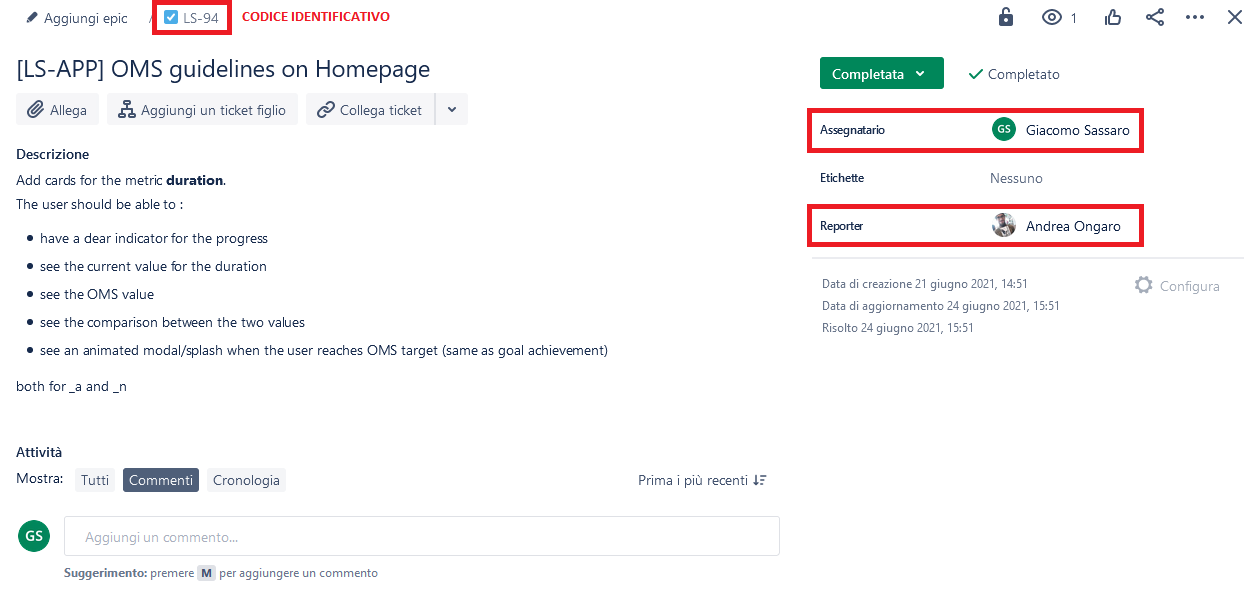
\includegraphics[height=6.5cm]{ticket}
    \caption{Esempio di ticket su Jira}
\end{figure}

Si è deciso inoltre di mantenere entrambe le applicazioni sullo stesso \textit{repository}, per questo motivo si sono dovute organizzare le cartelle in modo da avere un ambiente di lavoro ordinato. La scelta è stata quella di mantenere nella \textit{root} del progetto delle cartelle contenti i file condivisi tra le due applicazioni, e di creare altre due cartelle: \textit{client} e \textit{coach} aventi come figli delle cartelle con lo stesso nome di quelle presenti nella \textit{root}. In queste ultime cartelle vengono raccolti i file utilizzati solamente da una delle due applicazioni.
La struttura è risultata quindi la seguente:
\begin{itemize}
    \item auth, contiene il Provider per l'autenticazione di entrambe le applicazioni
    \item models, contiene le classi del modello di entrambe le applicazioni
    \item pages, contiene i widget \textit{fullscreen} utilizzati da entrambe le applicazioni
    \item widget, contiene i widget utilizzati da entrambe le applicazioni
    \item client, cartella contenente i file per l'applicazione client
    \begin{itemize}
        \item providers, contiene i provider dell'app client
        \item models, contiene le classi del modello dell'app client
        \item pages, contiene i widget \textit{fullscreen} dell'app client
        \item widget, contiene i widget utilizzati dell'app client
    \end{itemize}
    \item coach, cartella contenente i file per l'applicazione coach
    \begin{itemize}
        \item providers, contiene i provider dell'app coach
        \item models, contiene le classi del modello dell'app coach
        \item pages, contiene i widget \textit{fullscreen} dell'app coach
        \item widget, contiene i widget utilizzati dell'app coach
    \end{itemize}
\end{itemize}
%**************************************************************
\section{Confronto framework AR}
\label{sec:scelta-framework-flutter}
\subsection{ARway}
unity 
riuso di codice
ti tira via

\subsection{ar\_flutter\_plugin}
\subsubsection{il nostro ar flut plug}
fork per asa 
"com.gorisse.thomas.sceneform:sceneform:1.21.0" 

%----------------------------------------------------------------
\section{integrazione asa ar flut plug}
\label{sec:progettazione-onboarding-primo-login}


%----------------------------------------------------------------
\subsection{flutter <-> ar flut plug}
\label{sec:autenticazione-tramite-auth0}
passaggio dati app mobilesyn con ar flut plug (assets etc)

[diagramma comunicazione plug in ar - flutter]


\begin{figure}[h!]
    \centering
    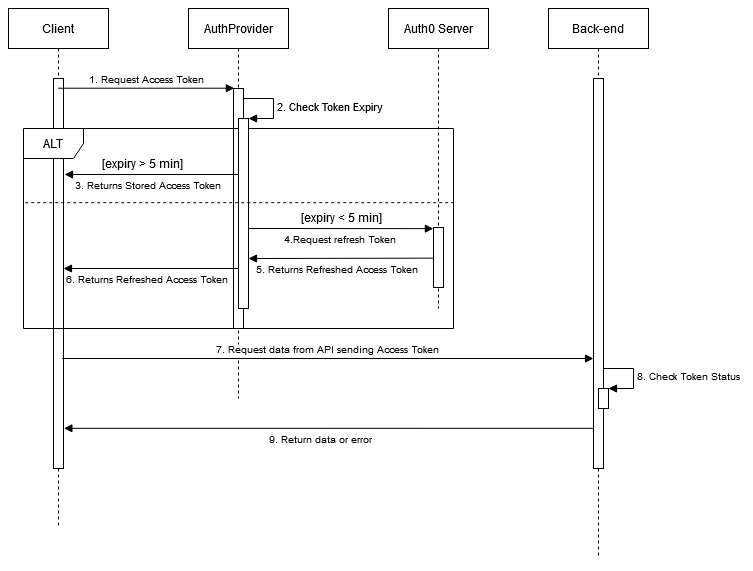
\includegraphics[height=10cm]{auth0}
    \caption{Diagramma di sequenza dell autenticazione usando auth0}
\end{figure}
\subsection{Chiamate asincrone}
Un punto chiave per lo sviluppo dell'app è quello delle chiamate asincrone.\\
Quando una funzione richiede molto tempo per essere completata, come ad esempio una funzione che richiede dati ad un un server, è opportuno chiamarla in modo asincrono, così da non fermare tutta l'applicazione in attesa del completamento di quella funzione. Utilizzando le chiamate asincrone infatti il flusso delle operazioni che non necessitano il termine della chiamata può continuare indisturbato.\\
Dart mette a disposizione due modi per la gestione di questo tipo di chiamate, noi in accordo comune abbiamo deciso di usare il metodo \textit{async} e \textit{await}: le funzioni che prevedono la possibilità di fare chiamate asincrone sono contrassegnate con la parola chiave \textit{async}. All'interno delle funzioni asincrone è possibile quindi usare la parola chiave \textit{await} che serve per dire al programma di attendere quell'istruzione prima di proseguire con la successiva. Se non viene utilizzato il comando \textit{await} allora tale funzione asincrona verrà eseguita parallelamente al proseguo del programma fino al suo completamento.\\
\begin{figure}[h!]
    \centering
    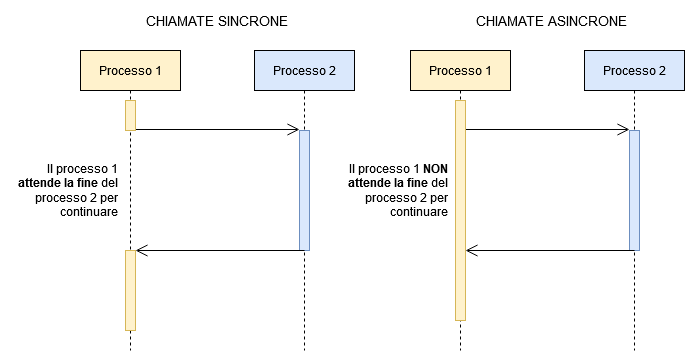
\includegraphics[height=6cm]{async}
    \caption{Chiamate sincrone VS asincrone}
\end{figure}
%*********************************************************************
\subsection{progettazione UI ux}

Essendo l'applicazione un supporto ad una piattaforma di analisi dati la presenza di chiamate asincrone al backend è molto frequente, è stato quindi fondamentale progettare un pattern solido da riutilizzare per ogni chiamata.
Il \textit{pattern} da noi adottato prevede che una qualsiasi chiamata API CRUD possa trovarsi in tre diversi stati:
\begin{itemize}
    \item \textbf{Loading}: la chiamata è iniziata e non è ancora stata risolta;
    \item \textbf{Error}: la chiamata è terminata con un errore;
    \item \textbf{Response}: la chiamata è terminata e possiedo i dati di mio interesse.
\end{itemize}
Appena prima di inviare la richiesta HTTP l'applicazione viene messa in uno stato di \textit{loading}, nel caso di errori al backend o nessuna risposta ci si troverà in uno stato di \textit{error}, altrimenti, nel caso in cui il backend risponda con i dati corretti ci si troverà in uno stato di \textit{response}.\\
L'interfaccia dunque cambierà in base allo stato della chiamata, mostrando un indicatore di progresso mentre ci si trova in uno stato di \textit{loading}, mostrando un errore nel caso ci si trovasse in uno stato di \textit{error}, o mostrando i dati elaborati nel caso di \textit{response}.
\begin{figure}[h!]
    \centering
    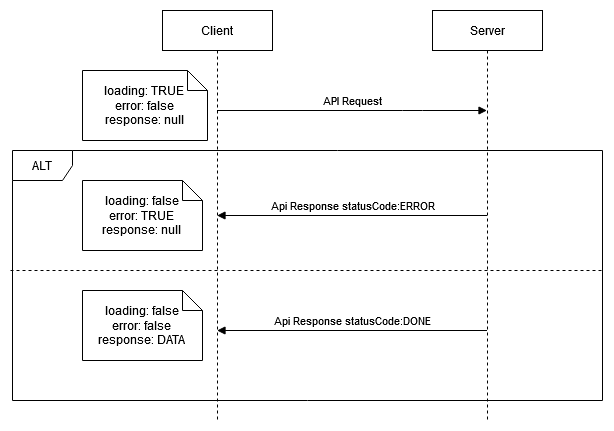
\includegraphics[height=8cm]{api}
    \caption{Diagramma di sequenza di una richiesta API}
\end{figure}
\begin{lstlisting}[language=dart, firstnumber=1,caption={User provider}]
final userChangeNotifier =
    ChangeNotifierProvider<UserRepo>((ref) => UserRepo(ref.read));
///Fornisce lo stato di errore di [UserRepo].
final userError = Provider((ref) => ref.watch(userChangeNotifier).error);
///Fornisce il messaggio di errore di [UserRepo].
final userErrorMsg = Provider((ref) => ref.watch(userChangeNotifier).errorMsg);
///Fornisce lo stato di loading di [UserRepo].
final userIsLoading =
    Provider((ref) => ref.watch(userChangeNotifier).isLoading);
///Fornisce l'istanza di [User].
final userProvider = Provider((ref) => ref.watch(userChangeNotifier).user);

class UserRepo extends ChangeNotifier {
  bool error = false;
  bool isLoading = false;
  String errorMsg = "";
  final String apiUrl = dotenv.env['API_URL'] ?? "";
  User? user;
  final Reader read;
  UserRepo(this.read);
  Future<void> fetchUser() async {
    var token = await read(authProvider).getAccessToken();
    this.isLoading=true;
	notifyListeners();
    try {
      final response = await Dio().get(
        apiUrl + "/api/myself",
        options: Options(
            headers: 
                <String, String>{'Authorization': 'Bearer $token'}),);
      if (response.statusCode == 200) {
        this.user = User.fromJson(response.data));
        this.isLoading = false;
      } else {
        this.isLoading = false;
        this.error = value;
        this.errorMsg = "richiesta fallita";
      }
    } catch (e) {
      this.isLoading = false;
	  this.error = value;
      this.errorMsg = "richiesta fallita";
    } finally {
	  notifyListeners();
    }
  }
}
\end{lstlisting}
%*************************************************************
\subsection{API di LifestyleSync}
Di seguito sono riportate alcune delle API utilizzate durante lo sviluppo delle applicazioni.\\
Esse si rifanno ad un modello REST-like e non REST puro in quanto tutte le richieste HTTP vengono firmate mediante la tecnica \gls{JWT} presentata in precedenza.\\
Le API verranno riportate nella forma [metodo\textunderscore HTTP][url/api]
\begin{enumerate}
    \item \textbf{GET api/myself}\\
    Restituisce un file JSON che descrive l'utente, con le sue info e i dettagli del suo coach, con il seguente schema:
    \begin{lstlisting}[language=json,firstnumber=1,caption={JSON schema dell'API GET api/myself},captionpos=b]
    {
    "user_id": String,
    "given_name": String,
    "family_name": String,
    "email": String,
    "picture": String,
    "info":
        {
        survey_done: bool,
        coach: Map<String, dynamic>,
        oms_thresh: Map<String, int>,
        fit_profiles: Map<String, dynamic>
        }
    "user_metadata": Map<String, dynamic>
    }
    \end{lstlisting}
    dove: \begin{itemize}
        \item user\textunderscore id: è l'identificativo dell'utente nel database;
        \item given\textunderscore name: è il nome dell'utente;
        \item family\textunderscore name: è il cognome dell'utente;
        \item email: è la e-mail dell'utente;
        \item picture: è il link dell'immagine del profilo dell'utente;
        \item user\textunderscore metadata: sono i meta-dati dell'utente;
        \item info:
        \begin{itemize}
            \item survey\textunderscore done: è true se l'utente ha completato il questionario;
            \item coach: sono i dati del coach dell'utente;
            \item oms\textunderscore thresh: sono le soglie da raggiungere secondo l'OMS;
            \item fit\textunderscore profiles: sono i profili fit dell'utente;
        \end{itemize}
    \end{itemize}
    \item \textbf{GET api/goals}\\
    Questa API accetta diversi parametri obbligatori:
    \begin{itemize}
        \item end: data di fine dei goals che voglio in formato \textit{IsoTime};
        \item active: se voglio i goals attivi o meno in formato \textit{Bool};
        \item interval: intervallo di tempo antecedente a \textit{end}, può essere: week, month, 3month o 6month in formato \textit{String}.
    \end{itemize}
    Restituisce un array di oggetti JSON che descrivono i goals dell'utente, con il seguente schema:
    \begin{lstlisting}[language=json,firstnumber=1,caption={JSON schema dell'API GET api/goals},captionpos=b]
    {
    "id": String,
    "u_id": String,
    "goals":
        {
        "calories":
            {
            "m": String,
            "thresh": int,
            }    
        "duration_activities":
            {
            "m": String,
            "thresh": int,
            }    
        "duration_normal":
            {
            "m": String,
            "thresh": int,
            }    
        "steps":
            {
            "m": String,
            "thresh": int,
            }    
        }
    "status":
        {
        "calories": int,
        "duration_activities": int,
        "duration_normal": int,
        "steps": int,
        }
    "start": IsoTime,
    "end": IsoTime,
    "achieved": bool,
    "active": bool,
    }
    \end{lstlisting}
    dove: \begin{itemize}
        \item id: è l'identificativo dell'obiettivo nel database;
        \item u\textunderscore id: è l'identificativo dell'utente nel database;
        \item goals:
        \begin{itemize}
            \item calories: sono le calorie da bruciare, \textit{m} è il tipo di metrica e \textit{thresh} è la soglia;
            \item duration\textunderscore activities: sono i minuti di attività da raggiungere, \textit{m} è il tipo di metrica e \textit{thresh} è la soglia;
            \item duration\textunderscore normal: sono i minuti attivi normali da raggiungere, \textit{m} è il tipo di metrica e \textit{thresh} è la soglia;
            \item steps: sono i passi da fare, \textit{m} è il tipo di metrica e \textit{thresh} è la soglia;
        \end{itemize}
        \item status:
        \begin{itemize}
            \item calories: sono le calorie bruciate;
            \item duration\textunderscore activities: sono i minuti di attività raggiunti;
            \item duration\textunderscore normal: sono i minuti attivi normali raggiunti;
            \item steps: sono i passi fatti;
        \end{itemize}
        \item start: è la data di inizio dell'obiettivo;
        \item end: è la data di fine dell'obiettivo;
        \item achieved: indica se l'obiettivo è stato raggiunto;
        \item active: indica se l'obiettivo è attivo.
    \end{itemize}
    \item \textbf{GET api/agendas}\\
    Questa API accetta diversi parametri obbligatori:
    \begin{itemize}
        \item end: data di fine degli appuntamenti che voglio in formato \textit{IsoTime};
        \item interval: intervallo di tempo antecedente a \textit{end}, può essere: week, month, 3month o 6month in formato \textit{String}.
    \end{itemize}
    Restituisce un array di oggetti JSON che descrivono gli appuntamenti, con il seguente schema:
    \begin{lstlisting}[language=json,firstnumber=1,caption={JSON schema dell'API GET api/agendas},captionpos=b]
    {
    "id": String,
    "start": IsoTime,
    "end": IsoTime,
    "subject": String,
    "tid": String,
    "notes": String,
    "coach": Map<String, dynamic>,
    "client": Map<String, dynamic>,
    }
    \end{lstlisting}
    dove: \begin{itemize}
        \item id: è l'identificativo dell'appuntamento nel database;
        \item start: è la data e ora di inizio dell'appuntamento;
        \item end: è la data e ora di fine dell'appuntamento;
        \item subject: è il titolo dell'appuntamento;
        \item notes: sono le note dell'appuntamento;
        \item tid: è il tenant a cui appartiene l'appuntamento;
        \item coach: sono i dettagli del coach;
        \item client: sono i dettagli del cliente.
    \end{itemize}
\end{enumerate}
%************************************************************
\subsection{Stato globale e locale}
Una delle problematiche principali quando si deve sviluppare un applicazione mobile o web è il come salvare i dati e gestire lo stato dell'applicazione.\\

Flutter prevede l’esistenza di due tipi di stato (simili ad uno \textit{store}): lo stato globale dell’applicazione, che ad ogni update causa un update dell’intero albero di \textit{rendering} dell’applicazione e lo stato locale, proprio del singolo widget e il cui update causa l’aggiornamento unicamente del widget stesso e dei suoi eventuali figli.\\
A seguito dell’analisi dei requisiti e del comportamento dell’applicazione si è deciso di utilizzare lo stato globale per i dati utilizzati da più widget con o senza legami di parentela. Mentre, seguendo il pattern \gls{SRP}, lo stato locale viene utilizzato dai widget che non condividono dati con altri componenti (ad esempio widget di pura presentazione o che rappresentano dati provenienti da un’API non sfruttata dall’intero applicativo).\\

Per la gestione dello stato globale abbiamo usato il provider pattern. Questo prevede l'utilizzo di un oggetto contenente i dati dell'applicazione che notifica ogni cambio di stato, il quale viene fornito all'applicazione utilizzando un \textit{provider}. In questo modo l'interfaccia grafica sarà sempre aggiornata con il valore corrente dello stato.\\
Per la gestione dello store globale si è deciso di utilizzare la libreria \textit{Riverpod}, questa fornisce una vasta scelta di \textit{provider} diversi, e rende più facile l'accesso ai dati grazie ad un hook da loro predisposto: \textit{useProvider}.
Per lo store locale invece, in seguito alla scelta di usare Flutter Hooks, abbiamo sfruttato l'hook \textit{useState}, questo costruisce una variabile che viene osservata dal componente, ad ogni cambiamento di questa variabile il componente si ricostruisce, aggiornandosi con il valore corrente dello stato.
%**************************************************************
\subsection{Routing iniziale}
Per questa prima parte del progetto è stato fondamentale progettare un buon routing per gestire correttamente i diversi casi di accesso.\\
Si è deciso per provare automaticamente il login all'avvio dell'applicazione utilizzando un token salvato nel \textit{secure storage} dello smartphone. Nel caso di accesso avvenuto con successo si prosegue, altrimenti si rimanda l'utente ad una schermata di login.\\
A questo punto è necessario controllare se è la prima volta che il cliente accede all'applicazione o meno, per fare questo controllo vengono richieste al \textbf{backend} le informazioni dell'utente e nel mentre viene mostrata una schermata di caricamento, a questo punto le possibili alternative di routing sono:
\begin{itemize}
    \item \textbf{Primo accesso}: viene mostrata all'utente una breve introduzione all'applicazione, gli viene presentato il suo coach, gli viene fatto rispondere ad un questionario rispetto al suo stile di vita e infine viene mandato all'homepage. Nel caso in cui l'esecuzione dell'app venisse interrotta prima del termine del questionario, l'accesso successivo sarà considerato nuovamente un primo accesso.
    \item \textbf{Altro accesso}: recupero i dati del cliente a cui viene mostrata l'homepage. In questo modo l'utente non ha più la possibilità di vedere l'introduzione all'app e di rispondere al questionario.
\end{itemize}
%***************************************************************
\section{Connessione ai device}
Altra tematica principale durante la fase di progettazione è stata quella della connessione della nostra app ai profili dei provider di fitness band e altri dispositivi in grado di rilevare passi, frequenza cardiaca e attività fisiche.\\
L’applicazione non prevede nessuna connessione diretta ai dispositivi, bensì ai profili dell’utente con i quali accede alle funzionalità di raccolta dati offerte dai provider. Ad esempio per rilevare i dati di durata di attività fisica e distanza percorsa da un utente che possiede una smartband Garmin, l’applicazione offrirà la possibilità di connettere il profilo LifestyleSync a quello Garmin.\\
Questa tematica era già stata trattata dall'azienda prima del mio arrivo e la soluzione scelta è stata quella di connettere la nostra app non direttamente ai device, ma all'account nelle rispettive app dei diversi device. Ossia, per rilevare i dati di una smartband di Garmin andiamo a collegare l'account del client in LifestyleSync al suo account nell'app Garmin.\\
I servizi che attualmente si prevede di utilizzare sono: Google Fit, Fitbit, e Garmin.\\
L'idea è stata quindi quella di progettare una sezione all'interno dell'app, in cui l'utente possa vedere a quali account è già associato e potrà quindi disconnettersi, e a quali account può collegarsi. Cliccando su uno di questi nel caso di disconnessione verrà fatta una richiesta POST al \textit{backend} che si occuperà della disconnessione, mentre nel caso di connessione l'utente verrà reindirizzato alla pagina di login del servizio scelto, una volta fatto il login verrà riportato alla pagina dell'app LifestyleSync e tramite una richiesta POST al \textit{backend} verrà fatta l'associazione.
%**************************************************************
\section{Dashboard utente}
L'app dovrà avere diverse sezioni principali: \textit{Homepage}, \textit{Move}, \textit{Food}, \textit{Health}; e altre secondarie: \textit{Agenda}, \textit{Chat}.\\
Abbiamo quindi fin da subito pensato di sfruttare una struttura a pagine.\\
Per fare ciò si è resa quindi necessaria una barra di navigazione e un componente per scorrere tra le diverse pagine.\\
Da qui si sono progettate ad una ad una tutte le diverse schermate.
\subsection{Homepage}
È la pagina principale, qui l'utente deve poter vedere un breve riassunto del suo percorso e del suo stato di movimento.\\
Dovrà quindi essere presente il nome del cliente con la sua immagine del profilo e un piccolo badge con un resoconto degli obiettivi in corso, falliti, completati e il badge relativo all'ultimo \textit{achievement} sbloccato.\\
Dovrà essere presente un indicatore dei minuti attivi settimanali a confronto con i minuti consigliati dall'OMS, la lista degli obiettivi attualmente attivi con la relativa scadenza e il progresso e la lista degli appuntamenti in arrivo.\\
Questa pagina deve essere facilmente scalabile con l'aggiunta di ulteriori informazioni.
\subsection{Move}
In questa pagina l'utente dovrà poter vedere tutti i suoi obiettivi legati al movimento.\\
Dovranno quindi essere presenti tutti gli obiettivi attivi e passati, per ogni obiettivo attivo dovrà potersi vedere il dettaglio e lo stato attuale, mentre per i passati il cliente dovrà poterli filtrare per data e per completamento, così da capire dove può migliorare e in che periodo è stato più produttivo.\\
Dovrà inoltre essere presente una schermata in cui il cliente possa vedere tutti gli \textit{achievement} relativi al movimento da lui sbloccati come se fosse una sorta di medagliere, quest'ultima opzione è stata pensata in ottica \gls{gamification}. 
\subsection{Food}
Questa pagina non è oggetto del mio progetto di tirocinio.\\
Dovranno essere presenti tutti gli obiettivi attivi e passati legati allo stato di alimentazione del cliente.\\
\subsection{Health}
Questa pagina non è oggetto del mio progetto di tirocinio.\\
Dovranno essere presenti degli indicatori sullo stato di salute del cliente, come l'andamento della frequenza cardiaca nell'arco della giornata.
\subsection{Agenda}
In questa pagina l'utente dovrà avere un resoconto di tutti i suoi obiettivi e appuntamenti nel calendario. Sarà quindi presente un calendario in cui per ogni giorno l'utente dovrà vedere i suoi appuntamenti e i suoi obiettivi.
\subsection{Chat}
Questa pagina non è oggetto del mio progetto di tirocinio a livello implementativo, mi sono occupato principalmente della progettazione.
In questa pagina l'utente può comunicare con il suo coach.\\
Sono stati analizzati diversi servizi ed \gls{SDK} per l'implementazione di un sistema di messaggistica, che in futuro dovrà anche gestire delle video chiamate.\\
Tra tutti i servizi analizzati si è pensato di utilizzare Google Firebase, in quanto rende possibile anche l'utilizzo delle notifiche push che possono tornare utili per altri scopi.
Qui il cliente avrà sempre aperta la chat con il suo coach, al quale potrà inviare messaggi testuali, foto, video o messaggi vocali. Per tutelare cliente e coach non si utilizzerà in alcun modo il numero di cellulare, la chat verrà gestite interamente da Google Firebase e dal nostro backend.\\
Inoltre per evitare che il coach si trovi troppi messaggi da tutti i suoi clienti, ogni cliente avrà una sorta di piano di abbonamento. Con l'abbonamento base gratuito avrà a disposizione un numero limitato di messaggi e minuti di chiamate al mese, mentre acquistando un abbonamento premium potrà aumentare il numero di messaggi e di minuti di chiamate.
%*************************************************************
\section{Applicazione coach}
La progettazione dell'applicazione coach segue la progettazione dell'applicazione client. Infatti viste le somiglianze e le funzionalità in comune tra le due applicazioni, si è deciso di utilizzare la stessa \gls{codebase}, e di sfruttare i flavors per compilare due diverse applicazioni a partire dallo stesso sorgente.\\
I flavors permettono di definire configurazioni di build separate che, tramite parametri e variabili d’ambiente, ci consentono di costruire l’applicazione distinguendo quali moduli fanno parte dell’applicazione coach e quali client. In questo modo possiamo inoltre selezionare icone diverse, indicare URL diversi per le API coach e client e generare \textit{appid} differenti per poter pubblicare negli store due applicativi differenti.
             % Concept Preview
% !TEX encoding = UTF-8
% !TEX TS-program = pdflatex
% !TEX root = ../tesi.tex

%**************************************************************
\chapter{Sviluppo}
\label{cap:sviluppo}
Il capitolo descrive le attività svolte e le principali difficoltà incontrate durate lo sviluppo delle applicazioni. Per prima verrà trattata l'applicazione cliente, in seguito l'applicazione coach e saranno disponibili gli screenshot dei risultati finali ottenuti.\\
La codifica è avvenuta per moduli: prima di passare al modulo successivo il risultato è stato visionato dall’azienda e dal tutor.\\
Saranno riportati solamente gli esempi di codice ritenuti più significativi.
%**************************************************************

\section{integrazione asa in ar flut plug}
La prima cosa su cui si è lavorato è stato il sistema di login e di recupero delle informazioni del cliente.\\
Una volta ricevuto dal mio tutor il \textit{provider} che si occupa del login tramite \textit{Auth0} sono stati sviluppati diversi widget per gestire il routing dell'applicazione in base al login avvenuto con successo o meno.\\
Inoltre è stato definito un modello per memorizzare i dati dell'utente ricevuto tramite chiamata API.
%*************************************************************************
\subsection{ar flutter plugin mobilesyn}
Per gestire il routing iniziale dell'applicazione si è deciso di sviluppare multipli widget \textit{statefull} in ascolto sullo stato di diverse richieste API, così facendo, al cambiamento di stato della richiesta API il widget viene ricostruito e indirizza l'applicazione ad un widget successivo in ascolto su di un'altra chiamata API. Questa opzione è stata scelta in quanto all'avvio dell'applicazione vengono eseguite diverse chiamate API e in questo modo è possibile osservare i campi \textit{Loading} ed \textit{Error}, come spiegato a sezione 4.3.3, in modo da avere un controllo sul flusso.\\
Di seguito elenco la lista di widget con i diversi instradamenti.\\
\begin{itemize}
    \item \textbf{MyApp}: prova l'autenticazione e finché il provider di autenticazione resta nello stato di \textit{Loading} mostra una \textit{SplashScreen}, successivamente indirizza verso il widget \textbf{CheckLogin};
    \item \textbf{CheckLogin}: controlla se l'accesso è avvenuto con successo o meno. Se si, in base al tipo di applicazione (client o coach) indirizza al widget \textbf{LoadUser} o \textit{LoadCoach}, se l'accesso è fallito indirizza alla \textbf{LoginScreen};
    \item \textbf{LoginScreen}: widget per riprovare l'accesso inserendo username e password;
    \item LoadUser: richiede al backend le informazioni dell'utente che ha effettuato l'accesso e mostra una schermata di caricamento mentre la chiamata è in stato di \textit{Loading}, successivamente indirizza al widget \textbf{CheckBoolUser};
    \item \textbf{CheckBoolUser}: controlla se è il primo accesso dell'utente o meno, se lo è indirizza ad una schermata con l'introduzione all'applicazione, altrimenti riporta alla schermata di \textit{Homepage}.
    \item \textbf{LoadCoach}: richiede al backend le informazioni del coach che ha effettuato l'accesso e mostra una schermata di caricamento mentre la chiamata è in stato di \textit{Loading}, successivamente indirizza al widget \textbf{CheckBoolCoach};
    \item \textbf{CheckBoolUser}: controlla se ci sono stati errori nel recupero delle informazioni, se ci sono stati restituisce un widget di errore, altrimenti riporta alla schermata di \textit{Homepage}.
\end{itemize}

\begin{lstlisting}[language=dart, firstnumber=1, caption={Widget CheckLogin}]
class CheckLogin extends HookWidget {
  @override
  Widget build(BuildContext context) {
    bool isLoggedIn = useProvider(authIsLoggedIn);
    bool error = useProvider(authError);
    String errorMsg = useProvider(authErrorMessage);
    if (error) return GenericErrorPage(errorMsg: errorMsg);
    if (!isLoggedIn) {
        return LoginScreen();
    } else {
      switch (envType) {
        case "client":
          return LoadUser();
        case "coach":
          return LoadCoach();
        default:
          return GenericErrorPage(errorMsg: "non sei ne coach ne client");
      }
    }
  }
}
\end{lstlisting}
%%%%%%%%%%%%%%%%%%%%%%%%%%%%%%%%%%%%%%%%%%%%%%%%%%%%%%%%
\begin{center}
\begin{figure}[H]
\subfloat[Splash Screen]{
\includegraphics[width = 4cm]{app_screenshot/splash_screen.jpg}} 
\hspace{0.1cm}
\subfloat[Waiter Screen]{
\includegraphics[width = 4cm]{app_screenshot/waiter.jpg}}
\hspace{0.1cm}
\subfloat[Login Screen]{
\includegraphics[width = 4cm]{app_screenshot/login.jpg}}
\caption{Prime schermate dell'applicazione}
\end{figure}
\end{center}
%%%%%%%%%%%%%%%%%%%%%%%%%%%%%%%%%%%%%%%%%%%%%%%%%%%%%%%%
A supporto di questi widget sono stati sviluppati tre widget fondamentali:
\begin{itemize}
    \item GenericErrorPage: accetta come parametro un messaggio di errore e presenta all'utente una generica pagina di errore con il messaggio passato come parametro;
    \item Waiter: accetta come parametro un messaggio e presenta all'utente una generica pagina di caricamento con il messaggio passato come parametro;
    \item DelayedWidget: accetta come parametro un numero di secondi ed una condizione da soddisfare. Alla costruzione del widget si avvia un timer della durata dei secondi passati come parametro. Mentre il timer è attivo o la condizione non è soddisfatta si presenta un widget di caricamento, solitamente \textbf{Waiter}, altrimenti viene mostrato all'utente un secondo widget passato anch'esso come parametro. Questo widget è fondamentale per evitare di avere caricamenti talmente brevi da non far vedere all'utente che l'applicazione sta recuperando dei dati.
\end{itemize}
\begin{lstlisting}[language=dart, firstnumber=1,caption={Classe DelayedWidget}]
class DelayedWidget extends HookWidget {
  final Widget child;
  final int timer;
  final bool condition;
  DelayedWidget({
    Key? key,
    required this.child,
    required this.timer,
    required this.condition,
  }) : super(key: key);
  @override
  Widget build(BuildContext context) {
    final timerCondition = useState(false);
    useEffect(() {
      Future.delayed(Duration(seconds: timer))
          .then((value) => timerCondition.value = true);
    }, []);
    if (timerCondition.value && condition)
      return child;
    else
      return Waiter(msg: "Caricamento");
  }
}
\end{lstlisting}

%*************************************************************************
\subsection{ui / ux}
La seguente classe è stata definita per contenere tutti i dati che l'applicazione necessita di conoscere rispetto all'utente che ha effettuato l'accesso. Nel caso dell'applicazione client, esiste una sola unica istanza di \textit{User} e questa viene fornita a qualsiasi widget la necessiti attraverso un provider dedicato.\\
Tale classe si compone di diversi attributi primitivi e di due attributi che sono istanze di altre classi:
\begin{itemize}
    \item \textbf{Info}: contiene le informazioni dell'utente tra cui anche un campo coach, istanza di una classe \textbf{Coach} la quale contiene i dati del proprio coach;
    \item \textbf{Metadata}: contiene i meta-dati dell'utente.
\end{itemize}
\begin{figure}[h]
    \centering
    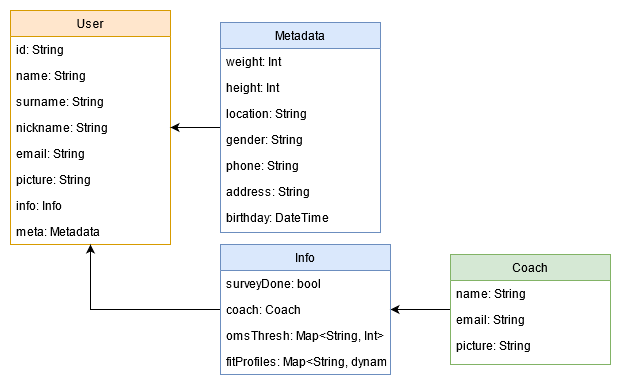
\includegraphics[height=8cm]{user_model}
    \caption{Modello di User}
\end{figure}
\subsection{Introduzione all'app e questionario}
Nel caso in cui sia il primo accesso di un utente, si è deciso di introdurlo all'utilizzo di LifestyleSync attraverso alcune schermate riassuntive delle principali funzionalità dell'applicazione.\\
Come ultima schermata inoltre viene presentato all'utente il coach che gli è stato assegnato, e successivamente gli viene presentato un questionario che è obbligato a compilare per continuare con l'utilizzo dell'applicazione.\\
Al termine del questionario le risposte vengono inviate al backend che si occupa anche di aggiornare le informazioni dell'utente segnando che ha completato il questionario, di conseguenza al prossimo login non dovrà ripeterlo e potrà utilizzare l'applicazione normalmente.\\
Per la realizzazione dei widget del questionario si è deciso di utilizzare una libreria anziché costruire tutte le diverse \textit{form} manualmente. Tra tutte le librerie trovate e provate la migliore si è rivelata \textit{SurveyKit}.\\
\textit{SurveyKit} rende disponibile un buon numero di widget altamente personalizzabili per diversi tipi di domande: risposta singola, multipla, radio button, checkbox, e via dicendo. Inizialmente non si sono presentati problemi nell'utilizzo di tale libreria, ma una volta terminato lo sviluppo si è presentato un bug, il quale porta al \textit{crash} dell`applicazione nel caso in cui l'utente annulli la compilazione del questionario.\\
Lo sviluppatore della libreria ha deciso di assegnare ad un tasto "Annulla" un metodo che va a rimuovere l'ultima pagina caricata nello stack del \textit{Navigator} di Flutter (Widget standard per la gestione del routing in Flutter) senza però controllare che una volta rimossa l'ultima pagina ce ne siano delle altre da presentare.\\
Nel nostro caso il questionario non viene caricato nello stack e di conseguenza, alla rimozione dell'ultima pagina caricata viene rimossa l'unica pagina caricata nello stack e di conseguenza l'applicazione va in errore e termina.\\
Per risolvere tale problema si è reso necessario il \gls{fork} della libreria e la rimozione del tasto "Annulla" dai diversi widget. Questo non risulta un problema in quanto l'utente è obbligato a compilare il questionario per proseguire nell'utilizzo dell'applicazione.\\
Generalmente viene sconsigliato il \gls{fork} di una libreria in quanto si perde la possibilità di mantenerla aggiornata con le future \textit{release}. Nel nostro caso però, avendo effettuato una minima modifica, ci rimane comunque possibile aggiornare la libreria alle future versioni ed eventualmente andare a ritoccare qualche riga di codice.\\
\newpage
%%%%%%%%%%%%%%%%%%%%%%%%%%%%%%%%%%%%%%%%%%%%%%%%%%%%%
\begin{center}
\begin{figure}[H]
\subfloat[Presentazione coach]{
\includegraphics[width = 4cm]{/app_screenshot/coach_info.jpg}} 
\hspace{0.1cm}
\subfloat[Domanda questionario]{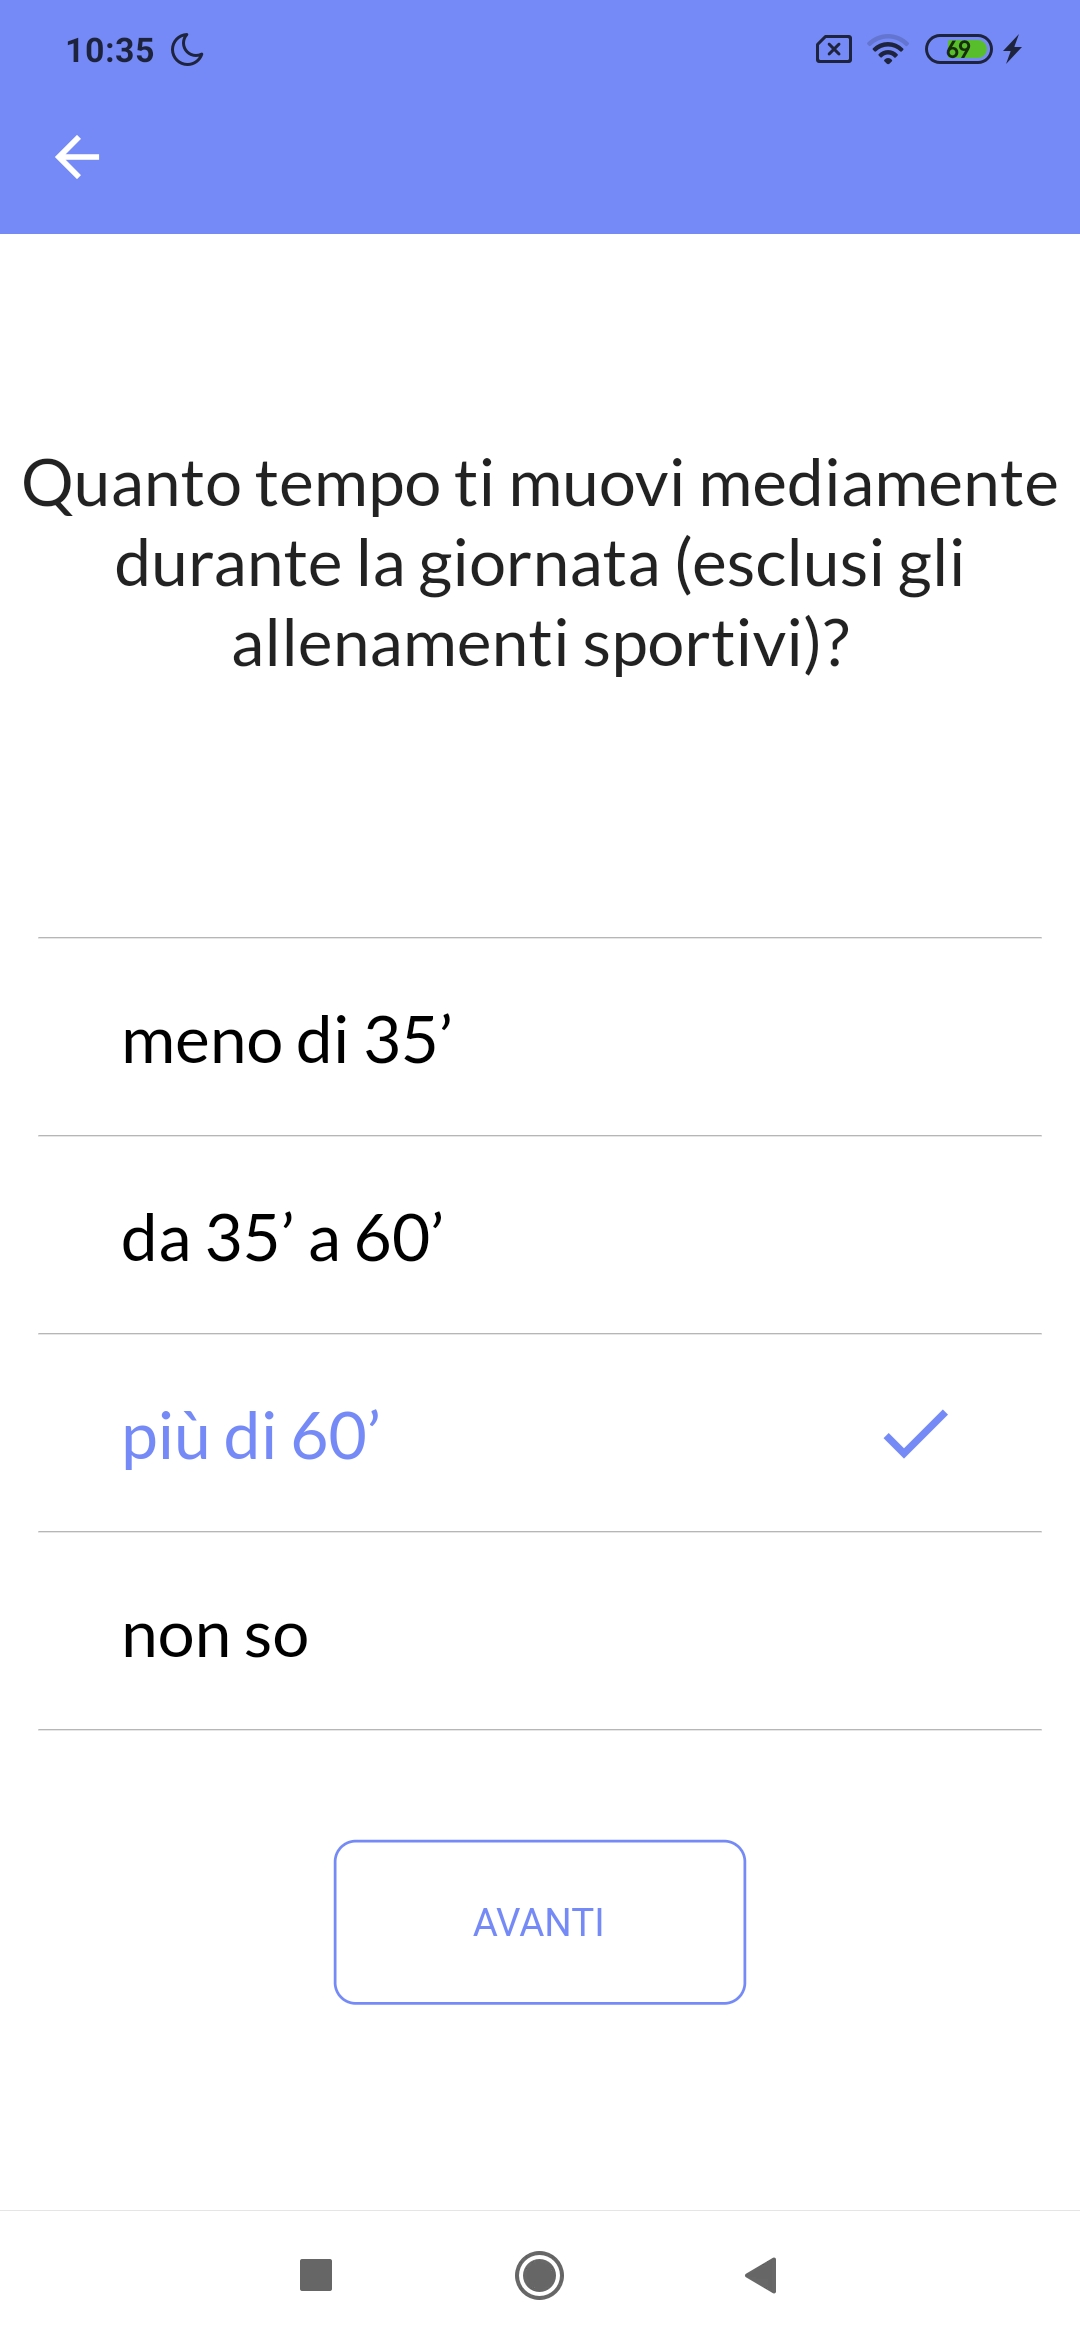
\includegraphics[width = 4cm]{app_screenshot/survey_question.jpg}}
\hspace{0.1cm}
\subfloat[Termine questionario]{
\includegraphics[width = 4cm]{app_screenshot/survey_done.jpg}}
\caption{Alcune schermate onboarding}
\end{figure}
\end{center}
%%%%%%%%%%%%%%%%%%%%%%%%%%%%%%%%%%%%%%%%%%%%%%%%%%%%%
%*************************************************************************
\section{Connessione ai device}
La connessione ai device è stata gestita per la maggior parte dal mio tutor in quanto aveva già utilizzato l'API per l'associazione del profilo LifestyleSync ai profili fitness nel sito web. Il mio compito è stato solamente quello di sviluppare l'interfaccia utente utilizzando i dati che mi venivano restituiti dal provider sviluppato dal mio tutor.\\
In fase di progettazione si pensava di connettere l'applicazione direttamente alle smartband dei diversi produttori (Google Fit, Fitbit, Garmin), in fase di sviluppo però ci si è resi conto che la connessione diretta al dispositivo fisico risultava eccessivamente complessa e si è deciso quindi di associare gli account delle diverse piattaforme di fitness all'account di LifestyleSync, così da prelevare le misurazioni delle smartband dai dati presenti negli account online e non direttamente dal dispositivo fisico.\\
È stata quindi sviluppata una sezione, nella schermata del profilo, attraverso la quale l'utente possa vedere a quali servizi è già connesso e può quindi disconnettersi o viceversa.\\
Nel caso l'utente provi la connessione a un nuovo servizio, premendo nell'apposito pulsante verrà aperta una pagina nel browser dello smartphone in cui è possibile effettuare l'accesso al servizio in questione e autorizzarne il prelievo dei dati. Nel caso in cui l'associazione vada a buon fine viene visualizzato un messaggio di successo e i dati iniziano ad essere salvati nel nostro backend, altrimenti viene visualizzato un messaggio di errore ed è necessario riprovare l'associazione.
\begin{figure}[H]
    \centering
    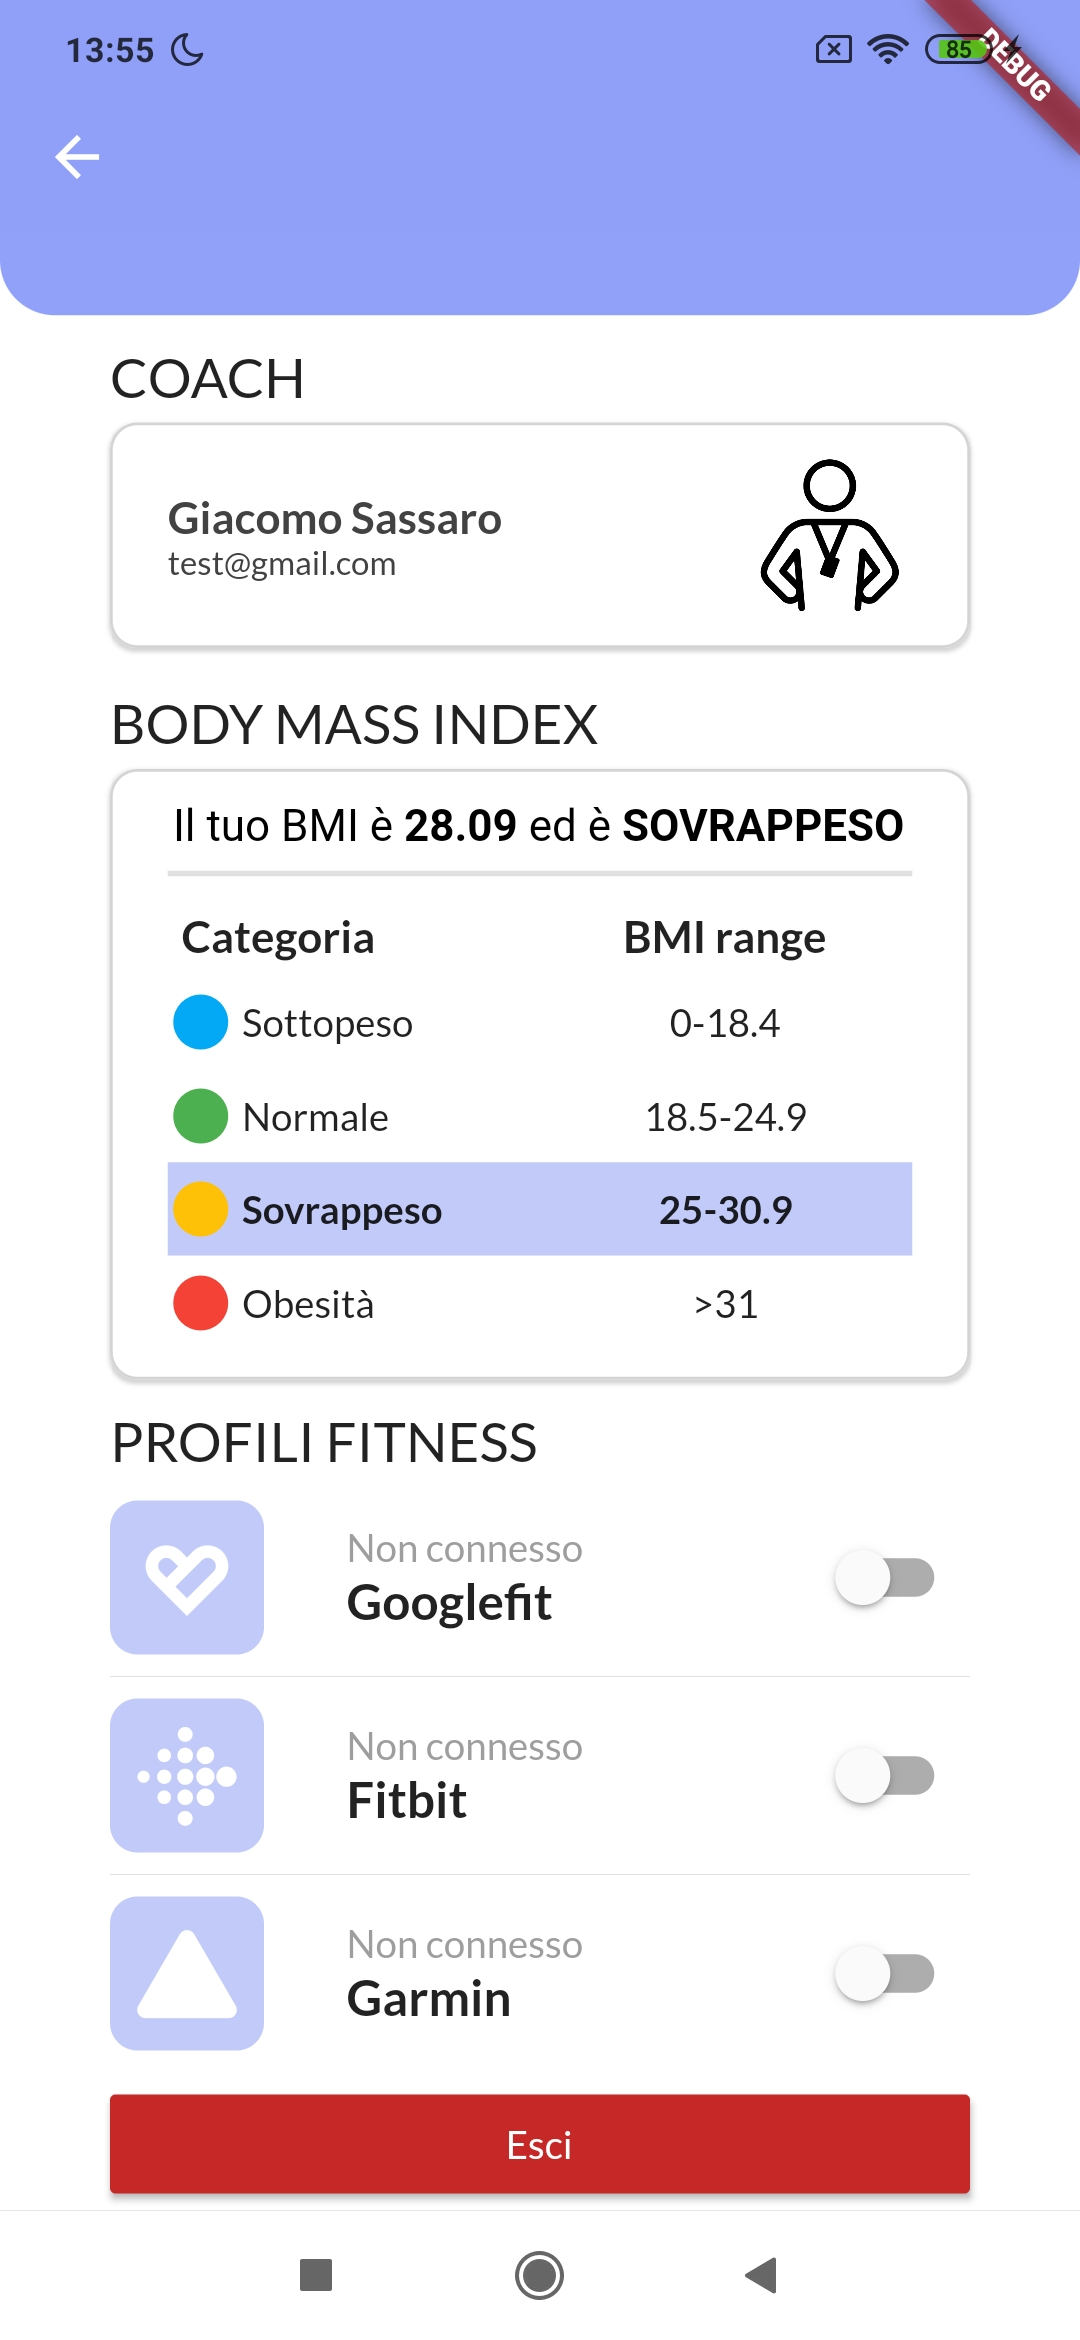
\includegraphics[width=4cm]{app_screenshot/profile_client.jpg}
    \caption{Schermata del profilo cliente con sezione relativa ai profili fitness}
\end{figure}
%*************************************************************************
\section{Dashboard utente}
Una volta completato lo sviluppo delle funzionalità Onboarding si è progredito con lo sviluppo della dashboard utente, ossia delle schermate principali con cui l'utente interagisce durante l'uso quotidiano dell'applicazione.
\subsection{Models}
Nelle varie schermate di dashboard utente sono visualizzati i diversi dati relativi a Obiettivi, Appuntamenti, Risultati e Attività. Tutti questi dati vengono richiesti al backend al caricamento dell'applicazione o nelle schermate che ne fanno uso, questo in base alla scelta progettuale di dove salvare i dati ricevuti: nello store globale o nello store locale di un widget.\\
Per memorizzare tali dati si sono dunque rese necessarie diverse classi: \textit{Goals}, \textit{Appointment}, \textit{Achievement}, \textit{Duration}
Siccome sia \textit{Appointment} che \textit{Goals} possiedono una data di inizio e una di fine, si è deciso di sviluppare una classe astratta \textit{Event} da cui farle ereditare. Questa scelta è stata fatta anche per permettere una scalabilità all'applicazione in quanto in futuro saranno sviluppate altre classi che avranno data di inizio e fine e potranno quindi anche loro ereditare da \textit{Event}.
\paragraph{Event}
Classe astratta rappresentate un evento generico.
\begin{itemize}
    \item \textbf{id}: identificativo dell'evento;
    \item \textbf{start}: data di inizio;
    \item \textbf{end}: data di fine.
\end{itemize}
\paragraph{Goals}
Insieme di obiettivi, questo insieme può essere attivo o passato e può essere stato raggiunto o meno. Attualmente un \textit{Goals} si compone di quattro \textit{Goal}: passi, minuti di attività, minuti non programmati, calorie.
\begin{itemize}
    \item \textbf{goals}: lista di \textit{Goal} indicizzata (steps, durationA, durationN, calories);
    \item \textbf{achieved}: obiettivo completato o meno;
    \item \textbf{active}: obiettivo attivo o meno;
\end{itemize}
\paragraph{Goal}
Un obiettivo da raggiungere che può essere: passi, minuti di attività, minuti non programmati, calorie.
\begin{itemize}
    \item \textbf{metric}: metrica di rilevazione;
    \item \textbf{thresh}: valore da raggiungere;
    \item \textbf{status}: valore attualmente raggiunto;
\end{itemize}
\paragraph{Appointment}
Rappresenta un appuntamento tra un \textit{Coach} e un \textit{Client}.
\begin{itemize}
    \item \textbf{subject}: titolo dell'appuntamento;
    \item \textbf{tenant}: gruppo di clienti al quale appartiene l'appuntamento;
    \item \textbf{notes}: appunti lasciati dal coach;
    \item \textbf{coach}: coach che partecipa all'appuntamento;
    \item \textbf{client}: cliente che partecipa all'appuntamento.
\end{itemize}
\paragraph{Duration}
Minuti di movimento di una giornata.
\begin{itemize}
    \item \textbf{id}: identificativo;
    \item \textbf{duration}: somma di durationA e durationN;
    \item \textbf{durationA}: minuti di attività giornalieri;
    \item \textbf{durationN}: minuti non programmati giornalieri;
    \item \textbf{ts}: data della rilevazione.
\end{itemize}
\begin{figure}[H]
    \centering
    \includegraphics[width=14cm]{models.png}
    \caption{Modelli dei dati}
\end{figure}
\subsection{Homepage}
Una volta predisposti i diversi modelli si sono sviluppati i widget per la rappresentazione di tali dati nell'homepage. Si è deciso di dare un resoconto di quasi tutti i dati nell'homepage, quindi mostrare tramite una card i minuti di movimento (durations), una lista di card con gli obiettivi (goals) e una lista di card con gli appuntamenti (appointment). \\
Da questa schermata l'utente può approfondire tutti i diversi ambiti cliccando su degli appositi widget. Cliccando sul proprio nome l'utente può vedere i dettagli del suo profilo, cliccando sul pulsante "Vedi tutti" di Obiettivi può visualizzare tutto il suo storico di obiettivi, ossia la sezione \textit{Move}, inoltre cliccando su una qualsiasi card può vedere i dettagli dell'evento premuto sia nel caso di un obiettivo sia nel caso di un appuntamento.
%%%%%%%%%%%%%%%%%%%%%%%%%%%%%%%%%%%%%%%%%%%%%%%%%%%%%
\begin{center}
\begin{figure}[H]
\subfloat[Homepage]{\includegraphics[width = 4cm]{immagini/app_screenshot/homepage_client.jpg}} 
\hspace{0.1cm}
\subfloat[Dettaglio obiettivo]{\includegraphics[width = 4cm]{immagini/app_screenshot/goals_details.jpg}}
\hspace{0.1cm}
\subfloat[Dettaglio appuntamento]{\includegraphics[width = 4cm]{immagini/app_screenshot/appointment_details.jpg}}
\caption{Homepage e dettagli eventi}
\end{figure}
\end{center}
%%%%%%%%%%%%%%%%%%%%%%%%%%%%%%%%%%%%%%%%%%%%%%%%%%%%%
\subsection{Move}
Questa schermata è raggiungibile dalla barra di navigazione o cliccando sul pulsante "Vedi tutti" degli obiettivi nella \textit{Homepage}. Qui si è deciso di presentare all'utente la lista di tutti gli obiettivi attivi, la lista degli obiettivi passati e una sezione con i risultati raggiunti e da raggiungere. Quest'ultima sezione è stata aggiunta in ottica \gls{gamification} in modo da spronare l'utente ad interagire con l'applicazione.\\
Per la sezione di obiettivi in corso si è potuto riutilizzare la card già sviluppata per l'\textit{Homepage}, mentre per la sezione di obiettivi passati si è deciso di sviluppare una nuova card e di aggiungere una form per la ricerca tra gli obiettivi passati. L'utente può decidere la data di fine, l'intervallo e il completamento per filtrare gli obiettivi passati.\\

%%%%%%%%%%%%%%%%%%%%%%%%%%%%%%%%%%%%%%%%%%%%%%%%%%%%%
\begin{center}
\begin{figure}[H]
\subfloat[Obiettivi attivi]{\includegraphics[width = 4cm]{app_screenshot/active_goals.jpg}} 
\hspace{0.1cm}
\subfloat[Obiettivi passati non raggiunti]{\includegraphics[width = 4cm]{app_screenshot/not_achieved_goals.jpg}}
\hspace{0.1cm}
\subfloat[Risultati]{\includegraphics[width = 4cm]{app_screenshot/achievement.jpg}}
\caption{Schermata Move}
\end{figure}
\end{center}
%%%%%%%%%%%%%%%%%%%%%%%%%%%%%%%%%%%%%%%%%%%%%%%%%%%%%
\subsection{Agenda}
Questa schermata è raggiungibile dalla barra di navigazione. Tale schermata è leggermente diversa nelle due applicazioni: i clienti possono vedere nel calendario sia gli appuntamenti sia gli obiettivi, mentre i coach vedono solamente gli appuntamenti in quanto non possiedono obiettivi.\\
Cliccando su un giorno del calendario vengono mostrate all'utente le card con obiettivi e appuntamenti di quel giorno, le card sono le stesse mostrate nell'\textit{Homepage}, si è potuto quindi riutilizzare buona parte del codice.\\
L'agenda è stata sviluppata in modo da essere altamente scalabile, è possibile infatti visualizzare gli eventi di tutto il mese o di settimana in settimana, inoltre nel caso in cui in futuro saranno aggiunti altri tipi di eventi sarà facile aggiungerli tra quelli visualizzati nel calendario.\\
La scalabilità è stata raggiunta utilizzando come oggetti da visualizzare nel calendario una lista di \textit{Event} e facendo un cast a runtime al tipo corretto di oggetto per costruire la card corretta.
\begin{lstlisting}[language=dart, firstnumber=1,caption={Costruzione delle card con individuazione a runtime del tipo}]
List<Widget> buildCards(List<Event> selectedElements, BuildContext context) {
    List<Widget> children = [];
    children.addAll(buildGoalsCards(
        selectedElements
            .where((element) => element is Goals)
            .map((e) => e as Goals)
            .toList(),
        context));
    children.addAll(buildAppointmentCards(
        selectedElements
            .where((element) => element is Appointment)
            .map((e) => e as Appointment)
            .toList(),
        context));
    return children;
  }
\end{lstlisting}
%%%%%%%%%%%%%%%%%%%%%%%%%%%%%%%%%%%%%%%%%%%%%%%%%%%%%
\begin{center}
\begin{figure}[H]
\subfloat[Agenda client]{\includegraphics[width = 4cm]{immagini/app_screenshot/agendas_client.jpg}} 
\hspace{0.1cm}
\subfloat[Agenda client una settimana]{\includegraphics[width = 4cm]{immagini/app_screenshot/agenda_one_week.jpg}}
\hspace{0.1cm}
\subfloat[Agenda coach]{\includegraphics[width = 4cm]{immagini/app_screenshot/agendas_coach.jpg}}
\caption{Homepage e dettagli eventi}
\end{figure}
\end{center}
%%%%%%%%%%%%%%%%%%%%%%%%%%%%%%%%%%%%%%%%%%%%%%%%%%%%%
\subsection{Chat}
Quest'ultima schermata è raggiungibile in entrambe le applicazioni dalla barra di navigazione.\\
Per i clienti, arrivati in questa schermata, è subito visibile la chat con il proprio coach ed è possibile inviare messaggi o media. Nel caso invece dell'applicazione coach, arrivati nella schermata della chat, è visibile una lista con i contatti di tutti i clienti e solo cliccando sopra una di questa voce si aprirà la chat con il cliente.\\
Purtroppo, viste le poche ore rimaste a disposizione per lo sviluppo di tale sezione, al momento è solamente possibile inviare messaggi di testo, foto e video grazie ad una libreria già sviluppata per Flutter che sfrutta \textit{Google Firebase}. Inoltre non essendo ancora integrato Google Firebase con il nostro backend, gli utenti della chat sono simulati e non sono in alcun modo collegati agli account di LifestyleSync.\\
La libreria utilizzata per la costruzione della chat, nonostante inizialmente si fosse rivelata valida, manca di molte funzionalità. Infatti nella libreria è implementato solo il messaggio di tipo testuale e immagine, ho dovuto quindi fare un \gls{fork} per implementare il messaggio video e in futuro sarà sviluppato anche il messaggio vocale.
%*************************************************************************
\section{Applicazione coach}
L'applicazione coach è stata sviluppata quando lo sviluppo dell'applicazione client era già iniziato da alcune settimane, buona parte delle componenti e delle schermate è stato quindi possibile riutilizzarlo apportando poche modifiche al codice. Si è deciso infatti di mantenere la stessa \gls{codebase} per entrambe le applicazioni e sfruttare i flavors.\\
La principale differenza di quest'app da quella dei clienti è che qui non sono presenti le schermate \textit{Move}, \textit{Food} ed \textit{Health} in quanto un coach non possiede obiettivi propri.\\
Nell'app coach è però presente una schermata in cui il coach può vedere tutti i suoi clienti con i relativi obiettivi a loro assegnati.\\
%%%%%%%%%%%%%%%%%%%%%%%%%%%%%%%%%%%%%%%%%%%%%%%%%%%%%
\begin{center}
\begin{figure}[H]
\subfloat[Homepage coach]{\includegraphics[width = 4cm]{immagini/app_screenshot/homepage_coach.jpg}} 
\hspace{0.1cm}
\subfloat[Lista clienti]{\includegraphics[width = 4cm]{immagini/app_screenshot/clients_coach.png}}
\hspace{0.1cm}
\subfloat[Dettaglio cliente]{\includegraphics[width = 4cm]{immagini/app_screenshot/client_details_coach.jpg}}
\caption{Schermate app coach}
\end{figure}
\end{center}
%%%%%%%%%%%%%%%%%%%%%%%%%%%%%%%%%%%%%%%%%%%%%%%%%%%%%
             % Product Prototype
% !TEX encoding = UTF-8
% !TEX TS-program = pdflatex
% !TEX root = ../tesi.tex

%**************************************************************
\chapter{Conclusioni}
\label{cap:conclusioni}
%**************************************************************
In questo capitolo vengono analizzati i risultati ottenuti durante l'attività di stage e vengono esposte le conclusioni tratte.
%**************************************************************
\section{Valutazione dei risultati ottenuti}
Il prodotto finale ottenuto rispetta le aspettative dell'azienda. L'interfaccia grafica risulta sobria e \textit{user-friendly}, inoltre grazie alla buona gestione dello stato dell'applicazione i rendering dei widget sono ben gestiti e non sono presenti rallentamenti nell'utilizzo dell'app.\\
L'app client e l'app coach rispettano tutti i requisiti funzionali obbligatori e desiderevoli delineati nell' Analisi dei Requisiti. Per quanto riguarda invece i requisiti di vincolo, per entrambe le app non è stato rispettato il requisito desiderabile \textbf{R2V3}: "L'applicazione deve funzionare completamente su dispositivi iOS". Questo è dovuto al poco tempo disponibile dedicato allo sviluppo per iOS, si è preferito infatti completare lo sviluppo e il testing per Android.
%**************************************************************
\section{Sviluppi futuri}
L'applicazione client una volta conclusa dovrà comporsi di tre diverse sezioni principali: Move, Food e Health.\\
Il mio stage ha coperto principalmente la sezione Move, predisponendo solamente delle schermate vuote per le altre due rimanenti.\\
I prossimi sviluppi saranno dunque la sezione di Food: sezione in cui il cliente avrà degli obiettivi alimentari da raggiungere e potrà vedere la sua cronistoria alimentare; e la sezione Health in cui il cliente potrà monitorare il suo stato di salute attraverso diversi grafici che andranno ad illustrare l'andamento del suo battito cardiaco nell'arco delle giornate e delle attività motorie.\\
Altra miglioria futura dovrà essere il \textit{restyling} grafico di alcuni elementi dell'applicazione che per mancanza di tempo si è deciso di lasciare solamente abbozzati.\\
Allo stesso modo anche per l'applicazione coach dovranno essere sviluppati degli elementi per raffigurare gli obiettivi di alimentazione e lo stato di salute di un cliente, per questa applicazione però non si dovranno produrre delle intere sezioni ma solamente alcuni elementi riassuntivi contenenti tutti i dati alimentari e di salute del cliente.\\
Invece per entrambe le applicazioni una funzionalità da sviluppare che andrà a dare grande valore al progetto è il sistema di messaggistica attualmente abbozzato. L'idea è quella di sviluppare un \gls{bot} che risponda automaticamente alle domande che più frequentemente vengono fatte dai clienti, mentre la chat diretta tra coach e cliente viene aperta solamente se il \gls{bot} non sa dare risposta ai dubbi del cliente.\\
Chiaramente il cliente non potrà abusare di questo sistema e avrà quindi un numero limitato di messaggi da poter inviare gratuitamente, al raggiungimento della soglia massima il cliente potrà sottoscrivere un abbonamento per aumentare il numero di messaggi inviabili.\\
Ultimo punto di estensione è la possibilità di effettuare delle video chiamate tra cliente e coach. Per quest'ultimo punto non è stata effettuata nessun tipo di progettazione ma l'idea è piaciuta all'azienda e in futuro verrà implementata.
%**************************************************************
\section{Conoscenze acquisite}
Durante il percorso di stage ho potuto approfondire le mie conoscenze di sviluppo mobile e di conoscere il framework Flutter.
Prima dello stage avevo già avuto l'occasione di sviluppare per dispositivi mobile e di utilizzare il framework React per la costruzione di interfacce grafiche web. Sicuramente la mia esperienza mi ha aiutato nell'iniziare il progetto e il percorso di stage mi ha permesso di migliorare nell'ambito dello sviluppo frontend per dispositivi mobile.\\
In particolare partecipando attivamente alla fase di progettazione e di realizzazione del prodotto ho imparato come si può strutturare un progetto complesso e che durante la realizzazione è importante fare attenzione a come le proprie scelte incidano sulla user experience del prodotto finale.\\
Dal punto di vista dell’integrazione all’interno dell’azienda, ho potuto acquisire nozioni sull’organizzazione e sulle fasi del ciclo di vita di un software, oltre alla possibilità di capire come relazionarsi all’interno di un team in ambito lavorativo.
%**************************************************************
\section{Utilizzo di Flutter}
L'esperienza con Flutter è stata positiva, infatti in seguito a qualche settimana di apprendimento mi è stato possibile costruire un'applicazione complessa in maniera semplice ed intuitiva. Inizialmente ho dedicato molto tempo al capire come funzionasse la gestione dello stato e delle chiamate asincrone, questa è stata la parte sicuramente più complessa nello studio del framework.\\ Mentre per la parte di gestione dei widget e di costruzione dell'interfaccia utente Flutter è molto semplice, grazie anche alla mia esperienza con React sono riuscito fin da subito a costruire schermate in modo intuitivo.\\

%**************************************************************
\section{Valutazione personale}
Questo stage è stato una buona esperienza formativa, ho avuto la possibilità di crescere a livello lavorativo sia acquisendo nuove competenze ma anche imparando a lavorare in un team nel quale è sempre stato possibile dialogare e scambiare idee.\\
Durante questa esperienza mi sono trovato spesso davanti a compiti che inizialmente non sapevo come affrontare ma che alla fine ho sempre portato a termine, penso dunque che le competenze fornite dalla laurea triennale siano una buona base dalla quale partire per studiare la maggior parte delle tecnologie usate in ambito lavorativo.             % Product Design Freeze e SOP
% !TEX encoding = UTF-8
% !TEX TS-program = pdflatex
% !TEX root = ../tesi.tex

%**************************************************************
\chapter{Appendice A}
%**************************************************************

\epigraph{Citazione}{Autore della citazione}




\fi
%**************************************************************
% Materiale finale
%**************************************************************
\backmatter
%\printglossaries
\printglossary[type=\acronymtype, title=Acronimi e abbreviazioni, toctitle=Acronimi e abbreviazioni]
\printglossary[type=main, title=Glossario, toctitle=Glossario]
% !TEX encoding = UTF-8
% !TEX TS-program = pdflatex
% !TEX root = ../tesi.tex

%**************************************************************
% Bibliografia
%**************************************************************

\cleardoublepage
\chapter{Sitografia}

\nocite{*}

% Stampa i siti web consultati
\printbibliography[heading=subbibliography,title={Siti web consultati},type=online]


\end{document}
